\documentclass[12pt, a4paper,twoside]{tesi_upf}

% added packages
\usepackage[inline]{enumitem}
\usepackage{booktabs,siunitx}
%\usepackage[inline]{enumitem}
%\usepackage{rotating}
%\usepackage{float}
% Quote packages
%\usepackage{quotchap}
\usepackage{csquotes}
\usepackage{courier}
\usepackage{epigraph}
\setlength\epigraphwidth{8cm}
\setlength\epigraphrule{0pt}
% Color assignment to names for revision
\usepackage[dvipsnames]{xcolor}
\newcommand{\alp}[1]{\textcolor{red}{#1}}
\newcommand{\toni}[1]{\textcolor{blue}{#1}}
\newcommand{\mireia}[1]{\textcolor{green}{#1}}
\renewcommand{\star}{{\usefont{OML}{cmm}{m}{it}\symbol{63}}}
% to add blank pages
\usepackage{afterpage}
\usepackage{setspace}
\usepackage{url}
\usepackage{enumitem}
\usepackage{listings}
\usepackage{hhline}
\usepackage{float}
\usepackage{amsmath}
\usepackage{subfig}

%listing style
\lstset{basicstyle=\footnotesize\ttfamily,breaklines=true, frame=single, columns=fullflexible}

%tick marks 
\usepackage{amssymb}
\usepackage{pifont}
\newcommand{\cmark}{\ding{51}}
\newcommand{\xmark}{\ding{55}}

% appendices
\usepackage[toc,page]{appendix}
\usepackage{tipa}
\usepackage{breakcites}

\usepackage{hyperref}
\hypersetup{
    colorlinks,
    linkcolor={red!50!black},
    citecolor={blue!50!black},
    urlcolor={blue!80!black}
}

%citation
\usepackage{natbib}
%\usepackage{apalike}
\usepackage{bibentry}
\nobibliography*

%CODIFICATION
\usepackage[utf8x]{inputenc}

%LANGUAGE
\usepackage[english,catalan,spanish]{babel}

%ONLY TO OBTAIN MARK BANK INDEX INDICATION A4
\usepackage[cam,a4,center,frame]{crop}

%INCLUDE GRAPHICS AND THE LOGO OF THE UPF
\usepackage{graphicx}

%FONTS TIMES OR GARAMOND, 
\usepackage{times}
%\usepackage{garamond}


%WITHOUT HEADINGS: NO MODIFICATION
\pagestyle{plain}

%FOR THE INDEX OF SUBJECTS
\usepackage{makeidx}
\makeindex

%CIRCLE AROUND CHARACTERS
\usepackage{tikz}
 
\newcommand*\mycirc[1]{%
   \begin{tikzpicture}
     \node[draw,circle,inner sep=1pt] {#1};
   \end{tikzpicture}}

%BIBLIOGRAPHY STYLE
\bibliographystyle{apalike}

%SELECT LANGUAGE
\selectlanguage{english}

%THE TABLE OF CONTENTS IS TITLE CONTENTS
\addto\captionscatalan
  {\renewcommand{\contentsname}{\Large \sffamily Sumari}}

%Paragraph skip amount
%\setlength{\parskip}{1em}
% Toni: This is what I always use: the plus and minus is to give some flexibility
\setlength{\parskip}{1ex plus 1pt minus 1pt}

% Toni
% Comment, if you prefer indent
%\setlength{\parindent}{0mm}


\usepackage{ulem}
\newcommand{\toniD}[1]{\textcolor{olive!50!black}{ \sout{#1}}}
\newcommand{\toniI}[1]{\textcolor{olive!50!black}{\uwave{#1}}}
\newcommand{\toniS}[2]{\toniD{#1} \toniI{#2}}
%\newcommand{\toniD}[1]{}
%\newcommand{\toniI}[1]{#1}
%\newcommand{\toniS}[2]{#2}


%ADD YOUR DATA
\title{Incorporating Prosody into Neural Speech Processing Pipelines}
\subtitle{Applications on automatic speech transcription and spoken language machine translation}
\author{Alp \"Oktem}
\thyear{2018}
\department{DE TECNOLOGIES DE LA INFORMACI\'{O} I LES COMUNICACIONS}
\supervisor{Dra. Mireia Farr\'{u}s i Dr. Antonio Bonafonte}

\begin{document}
\pagenumbering{gobble}

\maketitle

\cleardoublepage

%%%%%% Dedication

\noindent Write here your dedication

\cleardoublepage

%%%%%% End dedication

% Acknowledgements
% ---------------------------------------------------------------------
\vspace{-5mm}
{\Large \sffamily Acknowledgements}
\vspace{3mm}

The course of my last four years until the very last moment of the writing of this dissertation has been nothing but a thrilling ride. 
A ride that felt at times as smooth as on a highway, sometimes like a steep mountain climb, other times as if I was on vast plain with no particular direction, and sometimes like exploring in a cave that needed some explosions here and there. Wherever the road went though, if there is one thing that I learned, it is that the way gives its rewards as long as I keep moving on. It is a relief looking back at it right now and I feel gratitude for many people that accompanied me on this journey. 

First of all, I would like to give thanks to my supervisors that assisted me along the way. Thank you Mireia for always believing in my capabilities and ideas. Your positive attitude and unconditional support has empowered me greatly in arriving to this point. Toni, I feel extremely lucky to have had the opportunity to work closely with you. I have learned so much in this period not just in terms of technical and methodical knowledge but also in terms of collaboration skills.

It was a priviledge to work besides the members of the TALN tribe this past four years. People that are so talented, hard-working and some also exceptionally good at partying. A round of special thanks goes to Francesco, Luis, Juan and Mónica for their key advices and companionship, and to Miguel, Roberto, Simon and Alicia for being the game-changers in helping me keep pace and help me set a direction when I needed it. 

My study would not have been possible without the financial support of DTIC and the workers that maintain it. Special thanks to Aurelio Ruiz for his support and also the management of the DTIC-Maria de Maetzu program which contributed an important share to my research. 

A great deal of motivation that help me realize my work has to be attributed to my colleagues in Col·lectivaT: Pelin, Federica, Güneş and Baybars. I feel very lucky and hopeful for the future collaborating with you.

I keep a deep gratitude for the city of Barcelona and all the people in it that made me feel home here during the course of my PhD: Carla, Bora, Kerim, Berkay, Batu, Nico, Cam, Lauri, Lisa, Paco, Kiket and Mona. 

A big, heartful thanks to my family for always believing in the path that I take and offering their support in every means possible. Thank you Abi, for showing me how cool science can be; Baba, for your pride in my actions and ideas; and Anne for your unconditional love and relentless call to joy.

And finally, my family here, Carmen. I owe much to the faith you have in me in realizing my dreams. Thank you for making it getting better all the time, even this dissertation. 



\newpage\leavevmode\thispagestyle{empty}\newpage
% ---------------------------------------------------------------------

\frontmatter

% Abstract
% ---------------------------------------------------------------------
\selectlanguage{english}
\section*{\Large \sffamily Abstract}

In this dissertation, I study the inclusion of prosody into two applications that involve speech understanding:~automatic speech transcription and spoken language translation. In the former case, I propose a method that uses an attention mechanism over parallel sequences of prosodic and morphosyntactic features. Results indicate an $F_1$ score of 70.3\% in terms of overall punctuation generation accuracy. In the latter problem I deal with enhancing spoken language translation with prosody. A neural machine translation system trained with movie-domain data is adapted with pause features using a prosodically annotated bilingual dataset. Results show that prosodic punctuation generation as a preliminary step to translation increases translation accuracy by 1\% in terms of BLEU scores. Encoding pauses as an extra encoding feature gives an additional 1\% increase to this number. The system is further extended to jointly predict pause features in order to be used as an input to a text-to-speech system. 

\textbf{Keywords:} prosody, automatic speech transcription, punctuation restoration, spoken language machine translation, bilingual spoken corpus

\selectlanguage{catalan}
\vspace*{\fill}
\section*{\Large \sffamily  Resum}

En aquesta tesi estudio la inclusió de la prosòdia en dues aplicacions que involucren la comprensió de la parla:~la transcripció automàtica de la parla i la traducció de la llengua oral. En el primer cas, proposo un mètode que utilitza un mecanisme d’atenció sobre seqüències paral·leles de característiques prosòdiques i morfosintàctiques. Els resultats indiquen una precisió de $F_1$=70.3\% en la generació de la puntuació. En el segon cas m'ocupo de la millora de la traducció de la llengua oral utilitzant la prosòdia. Un sistema neural de traducció automàtica format amb un corpus de text en el domini del cinema s’adapta amb característiques de pauses afegides utilitzant un conjunt de dades bilingües prosòdicament anotada. Els resultats mostren que la generació de puntuació prosòdica com a pas previ a la traducció augmenta la precisió de la traducció en un 1\% en termes de BLEU. La codificació de les pauses com a característica addicional encara incrementa la precisió en un altre 1\%. A més a més, amplio el sistema de traducció per a predir conjuntament les característiques de pausa i poder-les utilitzar com a entrada en un sistema de síntesi de veu. 

\textbf{Paraulas clau:} prosòdia, transcripció automàtica de la parla, restauració de la puntuació, traducció automàtica de llenguatge oral, corpus bilingües

\vspace*{\fill}

\selectlanguage{English}




\newpage\leavevmode\thispagestyle{empty}\newpage
% ---------------------------------------------------------------------

% Table of contents
% ---------------------------------------------------------------------
\tableofcontents
% ---------------------------------------------------------------------

% List of figures
% ---------------------------------------------------------------------
\listoffigures
\addcontentsline{toc}{chapter}{Figures index}
% ---------------------------------------------------------------------

% List of tables
% ---------------------------------------------------------------------
\listoftables
\addcontentsline{toc}{chapter}{Tables index}
\newpage\leavevmode\thispagestyle{empty}\newpage
% ---------------------------------------------------------------------

\mainmatter

% CHAPTER 1: INTRO
% ---------------------------------------------------------------------
%**************** Introduction ******************
\chapter{Introduction}
\label{chapter:intro}

%Background: technology that converts speech into written form
%background1: human machine colaboration
Human machine collaboration has arrived to another level with the advent of natural language processing (NLP). By teaching machines to understand and interpret human languages, we can now solve many problems that before required human labour. For example, dialog systems help solve our queries the same way we are used to interact with a person, or machine translation has changed the way we perceive language barriers. Technology like automatic speech recognition and text-to-speech synthesis has made this interaction further possible in the spoken form of human languages. Automatic speech transcription, for example, involves conversion of speech to its written form and is applied in many type of applications such as dictation systems, automatic captioning and spoken dialogue systems. Spoken language machine translation (SLMT) involves automatic speech transcription as its first step but further translates the transcription into a second language and in some cases synthesize it. Its uses include, for example, automatic subtitling and automatic dubbing.

%Problem: During conversion, information is lost
As machines function using a pre-defined set of symbols, language in its written form dominates the functioning of most of these applications. Even in the cases where spoken language is involved, machines rely on a step where speech has to be converted to text in order to carry on with the subsequent processes in the pipeline. However, this conversion brings with it a loss of a dimension in the language. Compared to written language, spoken language inherently carries more information than its linguistic content. Linguistic units like words are enveloped within properly divided measures, accompanied with a certain melody that has its ups and downs delivered in a rhythm. These ``music-like'' aspects, which roughly correspond to ``prosody'' in language, deal with \textit{how} a certain utterance is delivered. It functions for structuring the spoken discourse and also to encode both linguistic and para-linguistic phenomena \citep{fujisaki2004}. Loss of this information in spoken language interfaced systems eventually harms the machine interpretation of the communicative intention as a whole. 

%This dissertation 
%If we desire to have machines understanding us in a complete way like humans do, this information residing in prosody needs to be processed besides the linguistic information.

\section{Motivation}

%Motivation and a short intro to prosody

The recent advances in automated processing of natural languages owe much to the application of neural networks. Although the core technology behind neural networks is not new, it has only recently started being preferred against older probabilistic methods in NLP and speech technology. This was largely due to the rise in computational power that made possible the training and applicability of the systems that use \textit{deep neural networks (DNN)}. Its use for language modelling was demonstrated in 2001 \citep{Bengio:LM}, for automatic speech recognition (ASR) in 2012 \citep{asr_dnnhmm} and machine translation (MT) in 2014 \citep{sutskever}. %Popularly used machine translation service \textit{Google Translate}\footnote{\url{http://translate.google.com}} uses DNN at its core since 2016 \citep{google_nmt}. 

As sketched in the introductory section, the current tendency in spoken language processing systems is carrying on with the modelling only the linguistic information once spoken input is converted to its written form. This causes an irreversible loss of the information that is encoded through prosodic features of speech, which are intonation, rhythm, and stress. 

I will demonstrate in this section the relevance of modelling of this level of language in two applications of spoken language processing: Automatic Speech Transcription and Spoken Language Machine Translation. Finally, I will touch on the issue of prosodic data compilation which is demanded in development of data-driven models that account for prosody. 

\subsection{Automatic Speech Transcription}
%ASR/punctuation motivation
The process of automatic speech transcription involves use of an ASR system to convert the spoken input to text. The raw text output of an ASR system generally lacks any form of punctuation. Depending on the application, punctuation proves to be important for two reasons: first, in the cases where transcriptions will be read by humans, lack of punctuation reduces readability to a large extent. This is demonstrated in the work of \cite{Tundik2018} where watchers of broadcast news were asked to compare punctuated and unpunctuated captions. Both for manually and automatically created transcriptions, punctuated transcriptions were preferred in helping follow the video content. Second case where punctuation has an important role is when the ASR output is further used in subsequent processes like machine translation or parsing. Both these processes require sentence-like units as input and cannot function with long unsegmented text. Furthermore, commas and other punctuation marks that are defined within the orthography of a language prove to be important cues for machines to understand text, similar to the case of humans \citep{Cho2017NMTbasedSA, Jones:1994:ERP:991886.991960}. Although rules of punctuation are formally defined within the grammatical and orthographic rules of a language, spoken language punctuation is predominantly related with prosody \citep{wallace}. Sentence structures and phrasing are often marked with intonational phrasing and breaks. Sentence modality influences the intonation style of a sentence, which in turn influences punctuation. Topic changes are generally marked with intensity and pitch resets \citep{Farrus:SP:2016}. Emphasized information is often delivered with stress. 

Looking at raw ASR output, which consists of only the linguistic content, is often not enough to determine punctuation especially in cases of spontaneous speech. This type of speech often does not follow a regular syntactic structure as in written language, thus making it difficult to determine punctuation based on syntactic or data-driven methods that are modeled for written text \citep{ballesterosneural}. Neural network-based work that gets use of prosodic cues report improvement in accuracy of the punctuation marks generated \citep{tilk2016bidirectional}, but still rely on huge chunks of textual data thus biasing models on written language. As they are the closest form of symbology that represents speech prosody in written form of language, its modelling requires a level in prosody. This calls for further study in the evaluation of various prosodic features on the task.  

\subsection{Machine Translation Enhancement with Prosody}
%Translation motivation
Spoken language machine translation (SLMT) is a type of machine translation architecture where input and/or output to the system is spoken language. In the speech-input setup, prosody is relevant for capturing the sentence structure and phrasing which in turn affects translations. In spoken-output systems the need to convey the prosodic structure into the synthesized speech appears in applications such as automatic dubbing. In both setups, a prosodic modelling of the input speech is needed to avoid the information loss at the recognition step. Prosodic transfer modelling was previously explored in a number of works \citep{aguero2006prosody, Quoc2018, anumanchipalli:2012}. The data used in these approaches are collected in laboratory conditions, meaning that recordings are prompted, and almost always are based on travel domain. There is no previous study that takes on a domain that involves more expressive speech such as movies or TV shows. Especially in these domains, there is a rich source of prosodic varieties that affect both translations for subtitling and dubbing. 

\subsection{Prosodic Data Compilation}
%Prosodic data collection
Key to machine learning-driven development is directly related to the availability of quality data. Although some toolkits exist that assist prosodic annotation of speech data \citep{Rosenberg10, ProsodyPro, L06-1340}, they fall short in terms of applicability in machine learning-based approaches. Another issue in prosodic data collection is that data collected in laboratory environments often fail in reflecting expressivity normally present in spoken language, and in turn, influence models to bias on unnatural data. To aid collection of expressive speech data, a form of harvesting ``found data'' that accommodates prosodic annotation is needed. Scalable methods to process, visualize and store this type of data is also necessary in developing data-driven methodologies.

\section{Objectives}
Revolving around the motivation that prosody should be incorporated in technology that involves spoken language understanding and processing, I have assigned the following objectives for the course of my research: 

\begin{itemize}
    \item Development of open tools that enable creation, prosodic annotation, handling and visualization of spoken language data.
    \item Compilation and publication of monolingual and bilingual corpora suitable for machine learning-based development that involves prosodic-linguistic modelling.
    \item Development of a framework for automatic punctuation restoration in  manually or automatically generated speech transcripts, using lexical and prosodic features.
    \item Assessment of the effect of acoustic-prosodic features on the quality of punctuation restoration and subsequent processes like dependency parsing and machine translation.
    \item Development of a machine translation framework for movie domain that enables prosodic feature input and output to aid translation and also to generate cues for synthesis.
\end{itemize}

My hypothesis is that systems that process spoken language will benefit from  modelling of prosodic features in speech besides the linguistic modelling involved in them. The experiments aim to assess this in neural network-based architectures. 

%Experiments based on neural nets 
\section{Outlining the Dissertation}

The rest of this dissertation is structured as follows:

\begin{itemize}
    \item \textbf{Chapter 2} first gives an overview on speech processing systems encompassing the motivated applications of this dissertation. Emphasis is given on deep neural network based-setups. Second, role and characteristics of speech prosody are reviewed. Finally, state-of-the-art in relation to my objectives are presented. 
    \item \textbf{Chapter 3} presents corpus related work. Tools that were developed and utilized for prosodic data compilation and visualization are presented. Also, two corpora that were used and published within the frame of this dissertation are explained in detail. 
    \item \textbf{Chapter 4} focuses on the topic of automatic punctuation restoration in raw speech transcripts with a focus on the use of prosodic features and their effects on recovery performance and parsing.
    \item \textbf{Chapter 5} explores the use of prosodic features within a neural spoken machine translation setting. 
    \item \textbf{Chapter 6} sets the final conclusions on the thesis in terms of the objectives reached and also outlines possible venues for future research and applications. 
\end{itemize}



\newpage\leavevmode\thispagestyle{empty}\newpage
% ---------------------------------------------------------------------

% CHAPTER 2: SoTA
% ---------------------------------------------------------------------
%**************** SoTA **************

\chapter{State of the Art}
\label{chapter:sota}
As presented in the introductory chapter, this dissertation focuses on two main applications: automatic transcription and spoken language translation. In the first part of this chapter, I will give an overview on the main research areas that are related to these two topics with a focus on neural network-based approaches. Automatic transcription, which is made possible with \textit{automatic speech recognition (ASR)}, is explained in Section \ref{sota:asr}. Approaches to the task of punctuation recovery in ASR output are presented in Section \ref{sota:punk_on_asr}. \textit{Neural machine translation} is presented in Section \ref{sota:nmt} with a focus on \textit{spoken language machine translation}. After a brief introduction to text-to-speech synthesis (TTS) systems in Section \ref{sota:tts}, I will present the concept of speech-to-speech translation with recent work on its field in Section \ref{sota:s2s}. Next, in Section \ref{sota:prosody}, I will give an overview on Prosody. Finally, the last part of this chapter reviews relevant work on the inclusion of prosody into these systems. Focus is given on usage of prosody in punctuation recovery in Section \ref{sota:punk_prosody} and adding prosodic modelling on spoken language translation in Section \ref{sota:prosody_in_smt}. 


\section{Neural Speech Processing Overview}
\label{sota:neuralspeech}
%speech processing systems overview

A spoken language system consists of at least one of the following modules: automatic Speech Recognition (ASR) for converting verbal communication into discrete symbolic form (i.e.~text), text-to-speech (TTS) system for generating information in spoken form, and a spoken language understanding (SLU) system for mapping between actions and verbal utterances \citep{slp_book}. Depending on the application, versions and combinations of these systems are employed to solve the task involved with it. For instance, an automatic subtitling system would involve an ASR system together with a speech activity detection module to transcribe the spoken parts in a media. If the subtitling is to be done in another language, the same pipeline would be followed by a machine translation system. A complete speech-to-speech pipeline would result in an automatic dubbing system where translated content would be synthesized using a TTS system. 

%neural networks overview. 
Research on these subareas of speech technology has recently experienced a great shift towards the usage of \textit{artificial neural networks (ANN)}. Popularity of ANN in general has risen in the recent years mostly due to advancements in computing power. Specifically, training of large and deep neural networks (DNN) in a reasonable amount of time has been made possible with \textit{Graphical Processing Units (GPUs)}.

I will introduce briefly the concept of DNNs as they form the basis of the experimentation presented in this dissertation. The information presented in this section can be consulted in \cite{shigeru2000handbook} and \cite{bengio_dl} for a \textit{deeper} understanding. 

\subsection{Deep Neural Networks}
\label{sota:dnns}

\begin{figure}[t]
  \centering
  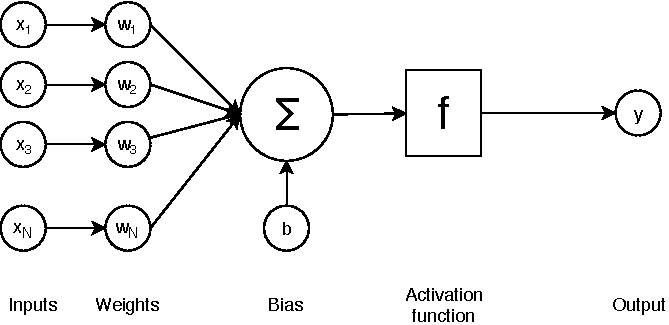
\includegraphics[width=0.6\linewidth]{img/perceptron.pdf}
  \caption{An artificial neuron.}
  \label{sota:neuron}
\end{figure}

An artificial neural network consists of a group of nodes and connections between them, inspired respectively by the neurons and axons in a biological neural system. Figure \ref{sota:neuron} illustrates the structure of one neural node, which is also referred as \textit{perceptron} or simply \textit{neuron}. Each connection towards a neuron is an input ($x_i$) and is associated with a weight coefficient ($w_i$). The basic function of a neuron defines the input signal to the neuron as:
\begin{equation}
    a = \sum _{ i }{ w_i x_i + b} 
\end{equation}

The input signal is then passed into an activation function to produce the output $y$. 

\begin{equation}
    y = f(a)
\end{equation}

Activation function is a differentiable function that originally resembles a step function so that the neuron \textit{fires} with certain input. The original Rosenblatt's perceptron had Heaviside step function as the activation function \citep{Rosenblatt58theperceptron}. Activation functions commonly being used today are the \textit{sigmoid} and the \textit{hyperbolic tangent} functions. 

One single neuron is evidently not sufficient for modelling complex functions. A basic neural network consists of a layer of input neurons fully connected to a layer of output neurons. This setting produces an N-to-M mapping. Extra layers are added between the input and output layers to introduce even more complexity to the network. These layers are called \textit{hidden layers} and are fully connected between each other between input and output layers. An illustration of a neural network with two hidden layers is given in Figure \ref{sota:neuralnet}. Number of hidden layers can be determined according to the task-at-hand. A neural network with more than one hidden layer is called a \textit{deep neural network} \citep{yoav}. 

\begin{figure}[t]
  \centering
  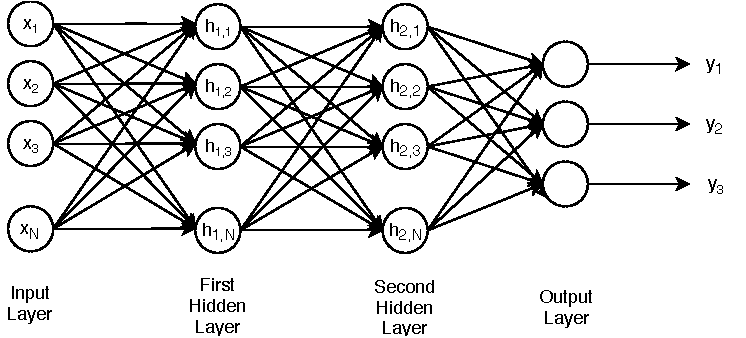
\includegraphics[width=0.9\linewidth]{img/NeuralNet.pdf}
  \caption{A fully connected feed-forward neural network with two hidden layers.}
  \label{sota:neuralnet}
\end{figure}

Although there exist many types of neural network taxonomies, one important characteristic that divides neural network architectures into two is the direction of the signal flow in the network. A \textit{feed-forward} network (as in the example in Figure \ref{sota:neuralnet}) allows information to be passed only in one direction, whereas a \textit{recurrent neural network (RNN)} network allows the output signal of some nodes to be passed again to a neuron coming previously, or to the neuron itself. Recurrent neural networks are especially suitable for representing time-series data. Because of this, it is currently being preferred as the principal architecture in many state-of-the-art applications of machine translation, speech recognition and speech synthesis. 

\begin{figure}[t]
  \centering
  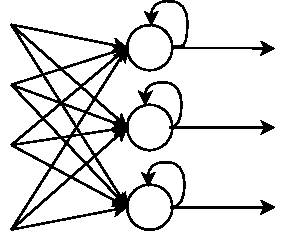
\includegraphics[width=0.3\linewidth]{img/RecurrentNeuralNet.pdf}
  \caption[Information flow in a recurrent neural network (RNN).]{Information flow in a recurrent neural network (RNN). Output signals are allowed to go back as input signals to the neurons. }
  \label{sota:rnn}
\end{figure}

As it can be seen in Figure \ref{sota:rnn}, a neuron in a RNN can have its output connected back to itself as an input. This model allows the neuron to keep a form of a \textit{memory} from previous inputs and decide on the next output according to it together with the current input. Modelling inputs and outputs in a time-series enables the processing of either a fixed number or a sequence of vectors, one at a time. Different types of RNN-based architectures is demonstrated in Figure \ref{sota:rnn_connections}. A one-to-one network serves for fixed size input and output at each time step. Although this architecture is useful in, for example, image classification, it is not sufficient for modelling variable length data. A ``many'' type input or output means an arbitrary number of vectors can be introduced to and/or obtained from the model at each time step. Many-to-many architecture can either have input and output sequences synchronized (left in the figure), where an output is given for each input vector, or not (right in the figure). An example to an non-synchronized many-to-many type architecture is machine translation. A sequence of vectors representing words in source sentence is first input to the model. Then, words from the translated sentence are decoded from the output layer. This group of neural networks are sometimes called \textit{encoder-decoder networks}. Many-to-many type RNN is sometimes referred to as a \textit{sequence-to-sequence network} as introduced in \cite{sutskever}. 

\begin{figure}[t]
  \centering
  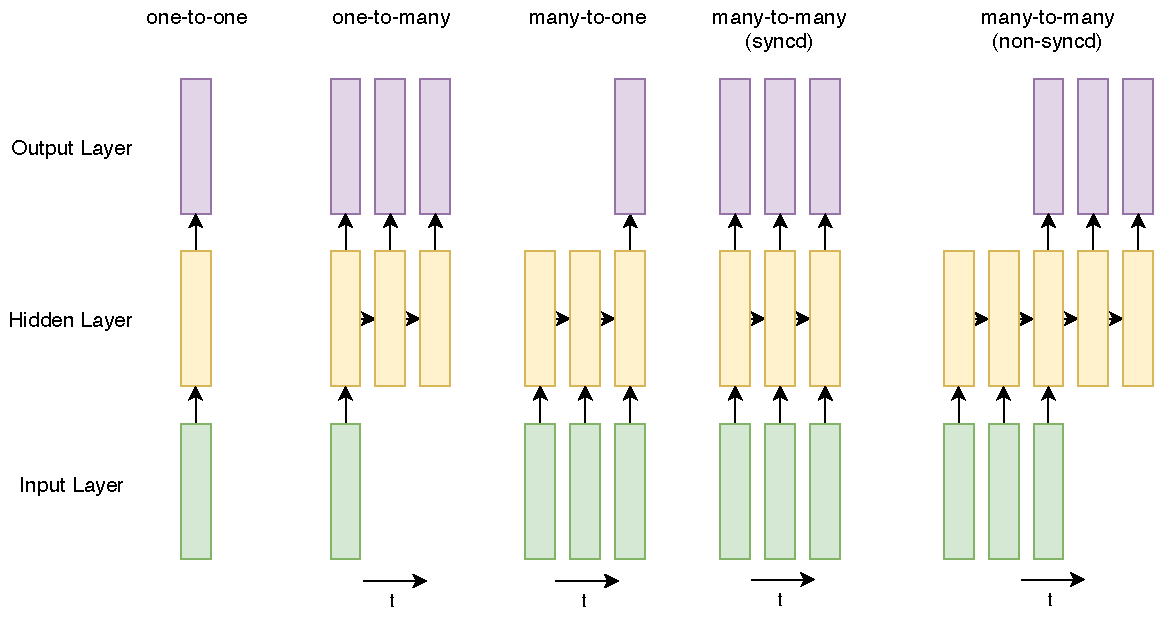
\includegraphics[width=\linewidth]{img/rnn_types.pdf}
  \caption[Various types of RNN architectures.]{Various types of RNN architectures. Each box represents a vector. }
  \label{sota:rnn_connections}
\end{figure}

%backpropagation
\subsubsection*{Neural Network Training}
The steps involved in neural network training can be summarized as follows: (1) introduction of samples in the training set to the network, (2) computing the error of the network regarding the desired and obtained output from the network, (3) computing the gradient given by the error and then (4) moving the network weights in the direction and magnitude of the gradient. 

The error of a network is calculated with the \textit{loss function}:

\begin{equation}
    E = \frac { 1 } { 2 } \left( y - f \left( \sum w _ { i } x _ { i } \right) \right) ^ { 2 }
\end{equation}

where $y$ represents the desired output, and $f(x)$ giving the output of the neural network. Using a method called \textit{backpropagation}, the error given by this function is traced back in the network layers using reverse differentiation. This is done by calculating the gradient of the loss function $\nabla J ( \theta )$ with respect to the weights $ \theta $ of the network.

Updating of the weights of the network is done with an \textit{optimization algorithm}. The \textit{gradient descent} technique is used to find the minima in an error space by updating the parameters of the network in the opposite direction of the gradient scaled with a learning rate $\eta$:

\begin{equation}
 \theta =  \theta -  \eta \cdot \nabla J(  \theta )
\end{equation}

As the calculation of loss with respect to the whole dataset would be cumbersome for large training sets, \textit{stochastic gradient descent (SGD)} \citep{bengio_dl, sgd2} does the parameter updates for each training sample $\{ x ( i ) , y ( i ) \}$:

\begin{equation}
    \theta = \theta -  \eta \cdot  \nabla J ( \theta  ;  x ( i  ) ;  y  ( i ) )
\end{equation}

However, this method causes unnecessary fluctuations (i.e.~noise) in weight updates as it is done at each input sample. To avoid this, samples are input in batches and the average loss for that batch is used to update the network instead.

Learning rate $\eta$ is a key hyperparameter in setting up neural network training. Optimization on the selection and variance of this parameter is often crucial in DNN architectures. \textit{Learning rate scheduling} is performed to help network converge with smaller updates through the later stages of training. Several variations on the SGD account for this aspect and further adapts the learning rate at each batch to each parameter. \textit{Adagrad} does this modification based on past gradients that were calculated for the parameters \citep{adagrad}. \textit{Adam} chooses an accelarated learning rate in relavant directions and diminishes it in irrelevant directions \citep{DBLP:journals/corr/KingmaB14}. 

\subsubsection*{Addressing the Problems of RNN}
There is a number of issues that has emerged in the development of RNNs and much of it is addressed in various works. First one is the issue that is common in any machine learning problem, which is \textit{overfitting}. A model is said to overfit on training data when it covers too well noisy data inside it and fails to generalize on anything outside it. Overfitting can be avoided by applying regularization techniques such as \textit{dropout} \citep{dropout}. This particular technique functions by randomly deactivating a portion of a layer's weights at each pass of a training sample, so that the network does not end up relying on specific weights \citep{bengio_dl}.

Two problems specific to the training of RNNs are \textit{exploding and vanishing gradients}. It is common that gradients end up either growing extremely high or extremely low during the course of backpropagation. The issue of exploding gradients is simply solved by putting a threshold on the magnitude of the gradients, and \textit{clipping} it once it is exceeded. On the other hand, resolution of vanishing gradient is still seen as an open research problem. Both these problems contribute to the shortcoming of RNNs in remembering long-term dependencies. \cite{longterm_is_difficult:1994} explores this issue in deep and stated the inefficiency of the gradient descent algorithm especially in preserving gradients across longer sequences. 

The issue with the short-term memory in RNNs was addressed with the introduction of \textit{Long-Short Term Memory (LSTM)} \citep{lstms}. LSTM defined a mechanism of \textit{gates} which decides on the information flow at each time-step. Gates decide which information is allowed to pass by through \textit{input} and \textit{output} gates, and which are bound to be discarded with the \textit{forget} gates. Although LSTM was an efficient solution for modelling long-term dependencies, it was also a complicated one \citep{bengio_dl}. Gated recurrent unit (GRU), was introduced as a simpler variant of LSTM units and made computation simpler by having fewer parameters \cite{gru}. Number of gates were reduced to two where the \textit{reset} gate determined whether the previous memory will be ignored, and the \textit{update} gate determines how much of the previous memory will be carried on. An illustration of architectures of both LSTM and GRU cells is given in Figure \ref{sota:figure:lstm_gru}.

\begin{figure}[t]
  \centering
  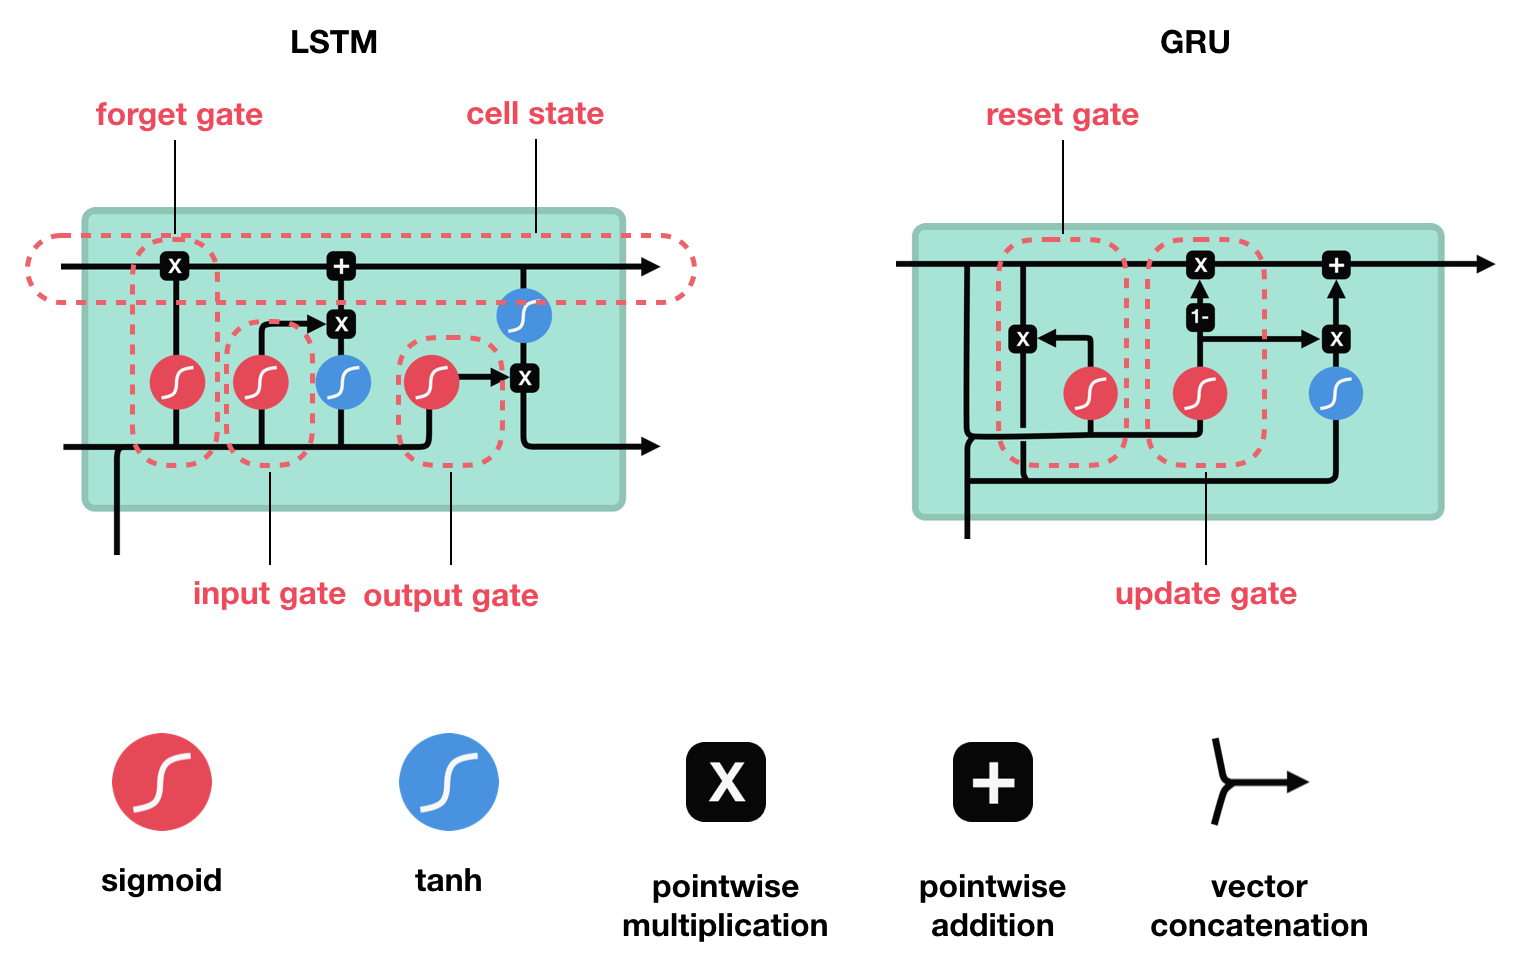
\includegraphics[width=0.85\linewidth]{img/lstm_gru.png}
  \caption[Architectures of a LSTM and GRU cell.]{Architectures of a LSTM and GRU cell. (Diagram from Michael Nguyen's article on Medium\protect\footnotemark)}
  \label{sota:figure:lstm_gru}
\end{figure}

\footnotetext{\url{https://towardsdatascience.com/illustrated-guide-to-lstms-and-} \url{gru-s-a-step-by-step-explanation-44e9eb85bf21}}

\subsection{Automatic Speech Recognition}
\label{sota:asr}

In its most simple sense, automatic speech recognition (ASR) is the conversion of speech in its acoustic form into a symbolic form such as words or letters. It is the probabilistic modelling of the question "What is the most probable word sequence among all possible word sequences given an acoustic input?". Figure \ref{sota:asr_process} illustrates this process. Speech signal captured by a microphone is first encoded into a sequence of acoustic feature vectors. Following, the acoustic feature vectors are decoded into the words that represent the linguistic information that lies in the speech signal. 

\begin{figure}[t]
  \centering
  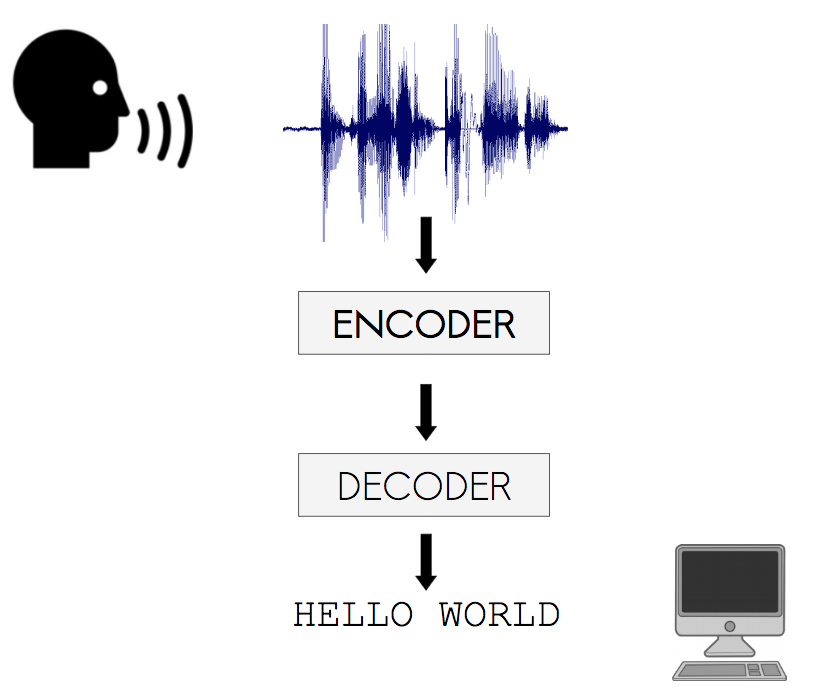
\includegraphics[width=0.5\linewidth]{img/asr_schema.png}
  \caption[Speech recognition.]{Speech recognition is the conversion of an acoustic signal with spoken language into its written form. }
  \label{sota:asr_process}
\end{figure}

Classical approaches to ASR employ a modeling of spoken language that uses Gaussian mixture model-hidden Markov model (GMM-HMM). HMM is a powerful statistical method for representing time-series data \citep{slp_book, hmm_balls}. As illustrated in Figure \ref{sota:asr_schema}, a GMM-HMM ASR system has a modular architecture: The feature extraction step converts the input speech signal into a sequence of fixed size acoustic vectors. Later, the decoder makes use of the acoustic model, the language model and the pronunciation dictionary in order to decide the most likely word sequences they represent. Acoustic and language models are trained with a corpus of transcribed speech samples and a text corpus respectively. While the acoustic model stores the information of the statistical behaviour of the sounds in a language, the language model stores the likelihood of the tokens (words) occurring and co-occurring in a language. 

\begin{figure}[t]
  \centering
  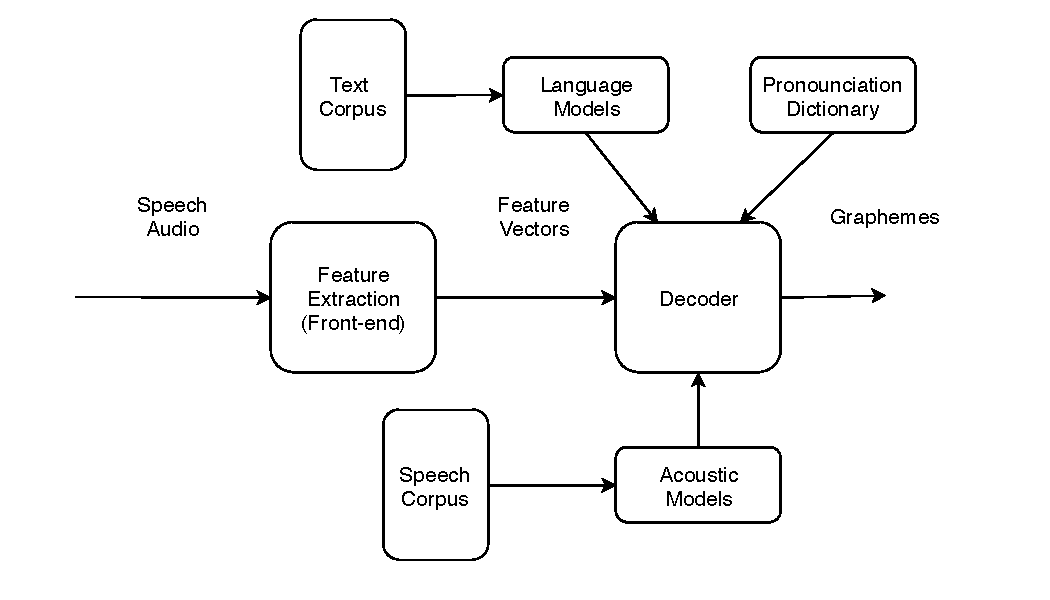
\includegraphics[width=0.8\linewidth]{img/asr2.pdf}
  \caption{General architecture of a traditional ASR system.}
  \label{sota:asr_schema}
\end{figure}

ASR systems experienced a breakthrough with the use of deep neural networks from 2012 on with its introduction in \cite{asr_dnnhmm}. The hybrid DNN-HMM model replaced the feature representation step that used Gaussian mixtures with a RNN-based architecture. The graphical comparison of the acoustic modelling of the two models is illustrated in Figure \ref{sota:gmm-dnn-hmm}. The DNN-HMM based ASR showed an improvement of 20\% in sentence accuracy compared to the GMM-HMM based model in a large-vocabulary task. 

\begin{figure}
\begin{tabular}{cc}
  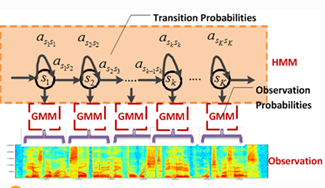
\includegraphics[width=0.5\linewidth]{img/gmm-hmm.png} &   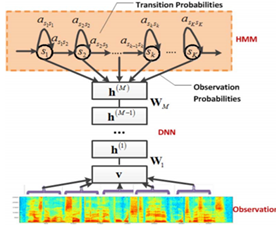
\includegraphics[width=0.5\linewidth]{img/dnn-hmm.png} \\
(a) GMM-HMM & (b) DNN-HMM\\[6pt]
\end{tabular}
\caption[Comparison between GMM based and DNN based ASR.]{Comparison between GMM based (a) and DNN based (b) ASR (Figure from \cite{asr_dnnhmm})}
\label{sota:gmm-dnn-hmm}
\end{figure}

More recently, end-to-end systems were introduced that made large-vocabulary speech recognition possible even without a language model or a lexicon \citep{e2e_asr}. Graves and Jaitly suggested a model that maps directly between spectral features and characters using a deep bidirectional LSTM and Connectionist Temporal Classification \citep{Graves:ctc} as loss function. Although this approach did not beat the hybrid approach baseline, it was a breakthrough for remedying a complex modular architecture that depended on separate acoustic, phonetic and language modelling. Later advancements, however, report outperforming of the hybrid methods both in terms of recognition accuracy and noise robustness \citep{deepspeech}.

\subsection{Punctuation Restoration in ASR Generated Transcripts}
\label{sota:punk_on_asr}

As applications of automatic speech recognition vary greatly, the objective of ASR is only focused on the recognition rate of the words. Aspects such as capitalization and punctuation, which are crucial elements for readability of the ASR output, is generally considered apart from an ASR system. For applications such as automatic captioning or transcript extraction, punctuation and capitalization prove to be essential for improving readability. In broadcast domain, \cite{Tundik2018} evaluate the effect of presence of punctuation in captions from an end-user perspective and show that punctuated captions are easier to read both when transcriptions are manually or automatically generated. In clinical domain, \cite{emrai} points out the importance of punctuation in the reports dictated by medical doctors. 

Another case where punctuation proves to be essential is when subsequent processing steps in spoken language system pipeline are optimized to work with it. Syntactic or semantic parsing, which is an important module in dialog based systems, necessitates input segmented into sentence-like units to function. Most machine translation systems are trained with single sentence input \citep{niehues2018}. Furthermore, it is proved that both of these processes function better with properly placed in-sentence punctuation and especially commas \citep{10045_76089, Jones:1994:ERP:991886.991960}. 

%from CSL
% TEXT
The problem of punctuation restoration has been addressed in several works in the literature --as has been the closely-related issue of boundary detection. Both problems have been tackled from diverse perspectives. In terms of which types of features are used, the approaches fall into three categories: (1) models based only on textual (lexical and syntactic) features, (2) models based only on prosodic/acoustic features and finally (3) models where both textual and acoustic/prosodic features are used. In this section, I will focus on models based only on textual features. That is, as illustrated in Figure \ref{sota:figure:punc_on_text}, punctuation process is only applied on the raw ASR output without any other cues. Models that employ prosodic features will later be explained in Section \ref{sota:punk_prosody}.

\begin{figure}[t]
  \centering
  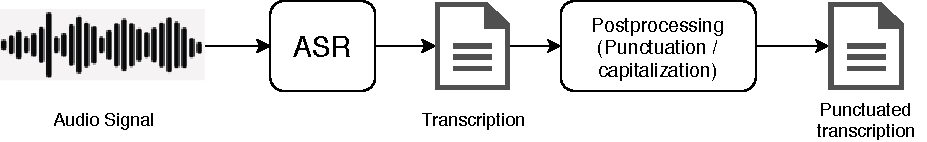
\includegraphics[width=\linewidth]{img/Punctuation_on_ASR_output.pdf}
  \caption{Punctuation and capitalization as a postprocessing step after ASR.}
  \label{sota:figure:punc_on_text}
\end{figure}

Punctuation using only textual features is relevant when e.g.~punctuation restoration is needed for written data \citep{jakubicek2010punctuation} or in the case when corresponding audio information is lost \citep{lu2010better}. In \cite{jakubicek2010punctuation}, for instance, the punctuation detection is addressed from a syntax-based perspective by using the output of an adapted chart parser, which provides information on the expected punctuation placement. In \cite{ueffing2013improved}, several textual features including language model scores, token n-grams, sentence length and syntactic information extracted from parse trees are combined using conditional random fields (CRF). They demonstrate that syntactic features help only when the input language is well-structured (as e.g.~newspaper texts). In \cite{lu2010better}, the task is based on dynamic CRF and applied to a conversational speech domain where sentence boundaries and types are detected. 

Another reason that facilitates the usage of solely textual features is the abundance of well-punctuated written data. Using a purely text-based n-gram language model, \cite{Gravano} demonstrate the performance improvement induced by large textual training in punctuation detection and capitalization. Although narrow-range grammatical constructions are recognized well for comma and period placement, n-gram approach fails in discovering long-range dependencies for the correct placement of question marks. 

Punctuation placement is also approached as a monolingual machine translation problem in \cite{peitz2011modeling, Cho2017NMTbasedSA, Paulik, Klejch} where target sequence is the punctuated version of the source sequence. 
  
Recently, usage of DNN-based systems has shown remarkable performance in the task for their ability to capture long-range dependencies in sequential data. These models use \textit{word embeddings} to represent words as vectors in a high-dimensional space that reflects their semantic, syntactic and morphological behaviour in the language \citep{mikolov_wordvec}. \cite{ballesterosneural} introduces a language-independent model with a transition-based algorithm using LSTM, without any additional syntactic features. \cite{Treviso} experiments with different word embeddings model within an RNN-based setup and proves that a good word embeddings model improves punctuation restoration accuracy. \cite{Che2016PunctuationPF} follows a convolutional neural network-based approach where the punctuation is predicted for the third word in a 5-word window and reports improvement on a similar non-DNN based approach that uses n-grams \citep{ueffing2013improved}. A task specific approach is followed in \cite{emrai} where punctuation marks are restored in medical dictation transcripts. They show that accuracy of state-of-the-art RNN-based methologies can be improved to a large extend using vocabulary reduction techniques adapting to the language domain. 

\subsection{Neural Machine Translation}
\label{sota:nmt}

Machine Translation is defined as the automatic conversion of a sequence of symbols in one language to a sequence of symbols in another language \citep{bengio_dl}. It has evolved through years from rule-based systems (RBMT) to statistical approaches (SMT), which modeled the probabilities of mappings between sub-phrases of various sizes. These probabilities are learned in a statistical fashion from \textit{parallel texts} where sentence aligned translations are available in the languages involved (referred as source and target languages). 

Neural machine translation (NMT) quickly replaced SMT in the recent years for its relatively simpler architecture and better performance. Usage of sequence-to-sequence architecture for this task was first introduced in \cite{sutskever} and made it to commercial spectrum in 2016 as the preferred architecture for the task \citep{google_nmt}. \textit{Transformer} architecture further simplified this model in and also recorded better performance \citep{transformer}.

%It no longer needed fine-tuning of smaller components involved in a SMT system and directly learned mapping from input text sequence to the target text sequence \citep{bahdanau, google_nmt}.

\begin{figure}[t]
  \centering
  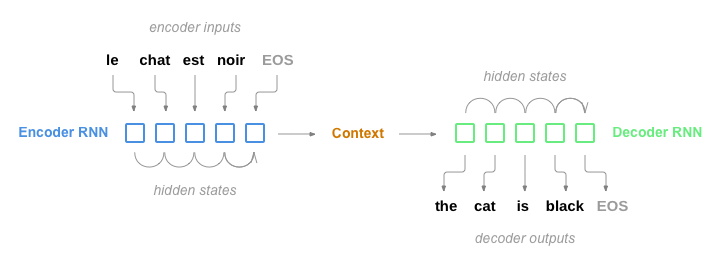
\includegraphics[width=\linewidth]{img/spro_nmt.png}
  \caption[Architecture of an encoder-decoder neural machine translation system.]{Architecture of an encoder-decoder neural machine translation system. (Diagram taken from \textit{spro}'s\protect\footnotemark sequence-to-sequence translation tutorial on github)}
  \label{sota:nmt_schema}
\end{figure}

\footnotetext{\url{https://github.com/spro}}

A commonly used architecture for NMT is the encoder-decoder architecture. As illustrated in Figure \ref{sota:nmt_schema}, token vector sequence in the source language input through an encoder is sent over to a decoder to output token vectors of the target language. Tokens can either represent words \citep{sutskever}, sub-word units \citep{google_nmt} or characters \citep{Ling2015CharacterbasedNM, marta}. Similar to the data-driven approach of SMT, this network is trained with parallel text, generally on sentence level, to maximize the probability of a correct translation given a source sentence \citep{bahdanau}.

\begin{figure}[t]
  \centering
  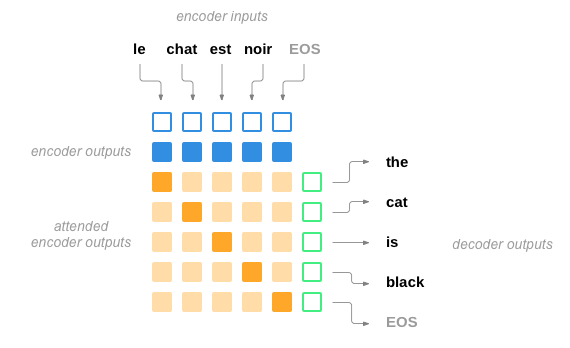
\includegraphics[width=0.8\linewidth]{img/spro_nmt_attention.png}
  \caption[Attention mechanism in encoder-decoder NMT architecture.]{Attention mechanism in encoder-decoder NMT architecture keeps track of portions of the input sequence that affects each decoder output. (Diagram taken from \textit{spro}'s sequence-to-sequence translation tutorial on github)}
  \label{sota:nmt_attention}
\end{figure}

One weakness that this model introduces is the connection between two RNNs that squeezes the input sequence into one single-length vector before being decoded as target token sequence. This is analogous to reading a phrase from beginning to end and then translating it into another language without looking at it again. Normally, a translator would break a input sentence into smaller portions and translate step by step giving attention to a different parts each time. An analogy of this approach was implemented in NMT with the introduction of \textit{attention mechanism} \citep{bahdanau, luong}. As illustrated in Figure \ref{sota:nmt_attention}, the attention mechanism helps focus on different parts of the input at each step of decoding. This relieves the decoder from having to predict target language tokens in one go without any spacial context of the input phrase \citep{google_nmt}. 

\textbf{Spoken language machine translation} is a type of MT where input and/or output to the system is spoken language. Spoken input translation can be employed through the usage of ASR prior to MT and translation can be generated as speech with a TTS to obtain spoken output. 

Machine translation with spoken input introduces its own specific challenges. First is that written and spoken domain show differences which could lead to degradation of performance if data domains are not compatible \citep{britz}. 

\begin{figure}[t]
  \centering
  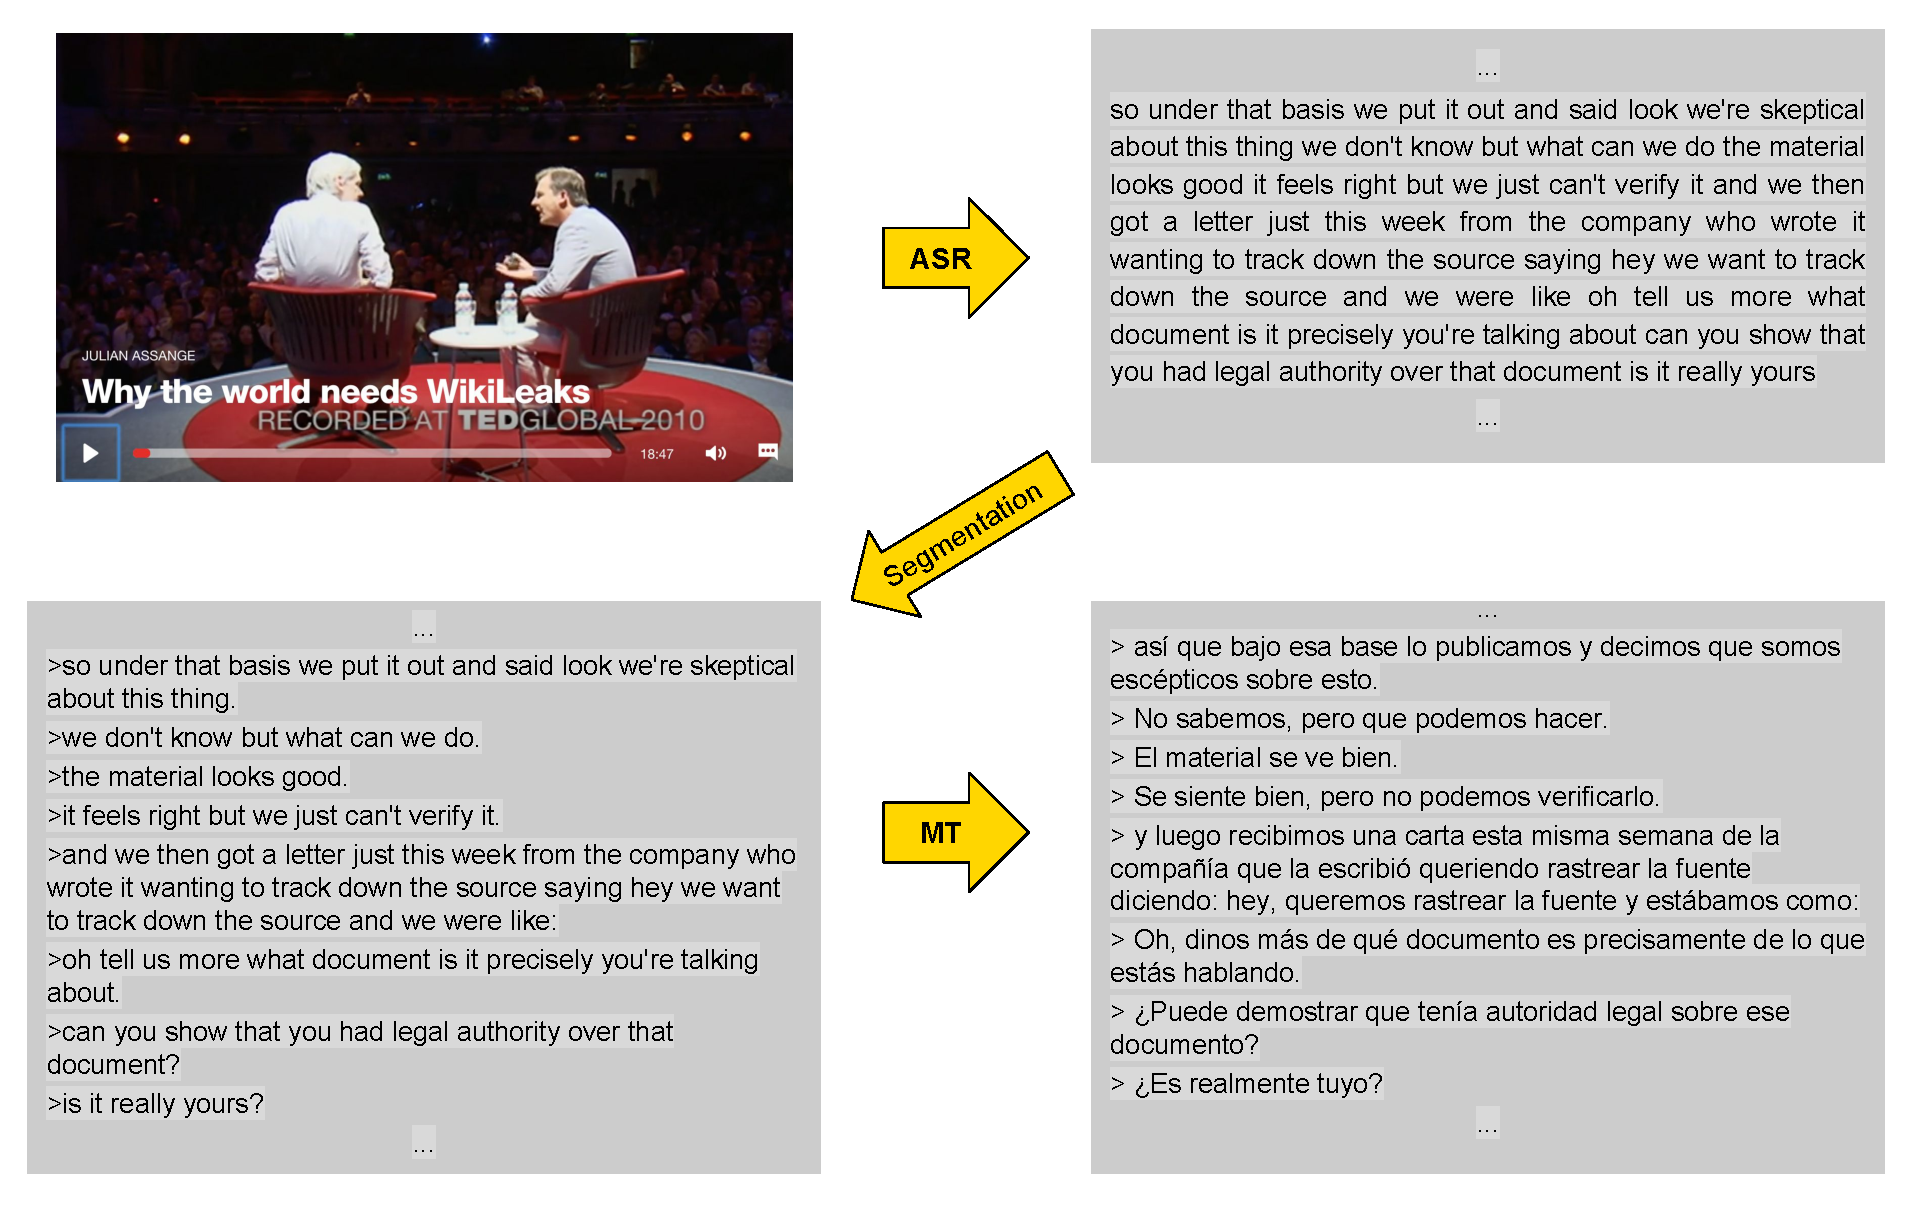
\includegraphics[width=\linewidth]{img/slmt_on_ted.pdf}
  \caption{Spoken language translation demonstrated on a conference recording.}
  \label{sota:tv_transcription}
\end{figure}

Another challenge that spoken language translation introduces is the possible incompatibility between ASR output structure and MT input structure. MT models are usually trained with sentence-like structures as samples and therefore show low performance on partial sentence or long sequences of words as input \citep{niehues2018}. In text translation domain, processing of long text documents is performed by translating it sentence by sentence using punctuation information as segmentation cues. A similar approach needs to be followed when input is spoken utterances as well. Figure \ref{sota:tv_transcription} illustrates an example of spoken language translation of a conference talk. A standard MT system would be unable to translate the unsegmented transcription of the talk. Translation is made possible only through a segmentation process, such as boundary detection or punctuation restoration. 

A topic worth mentioning in the area of translation is methods for measuring the accuracy of automatic machine translation methods. Commonly used metrics like \textit{BLEU} offer a remedy for the expensive labour involved in human evaluation of translation. The evaluation is performed in comparison with human translations. Given a testing set, each machine translated sample is compared to a reference translation and given a score of how close they are. \textit{BLEU} that stands for \textit{Bilingual Evaluation Understudy} measures this by calculating the ratio of matching n-grams in the translation and reference text \citep{bleu}. A BLEU score is basically a number between $0$ and $1$, $1$ signifying a higher similarity between the texts. The quality of a MT system is usually estimated with an average score among a set of testing samples and reported in percentage. 

\subsection{Text-to-Speech Synthesis}
\label{sota:tts}

%TTS:concatenative TTS
Speech synthesis involves production of a human-like speech given a text input with computational methods. Before the advent of deep learning, there were two main approaches to text-to-speech (TTS) synthesis: concatenative TTS, and parametric TTS. Concatenative TTS, also called unit selection, combines short pre-recorded audio clips called units to synthesize the desired text \citep{vanSanten:1997:PSS:241679}. Figure \ref{sota:figure:concatenative_tts} illustrates this process. A linguistic analysis performed on the text dictates which units to be selected in which order to form the waveform from an audio codebook consisting of phones, biphones or triphones. Since audio units are based on real speech samples, this technique can provide a good performance in terms of speech quality. That is, it sounds very similar to real human speech. However, the cut and stitch procedure involved often results in lack of naturalness. Also, this technique proves to be less flexible since its construction involves creation of a carefully designed large database. 

\begin{figure}[t]
  \centering
  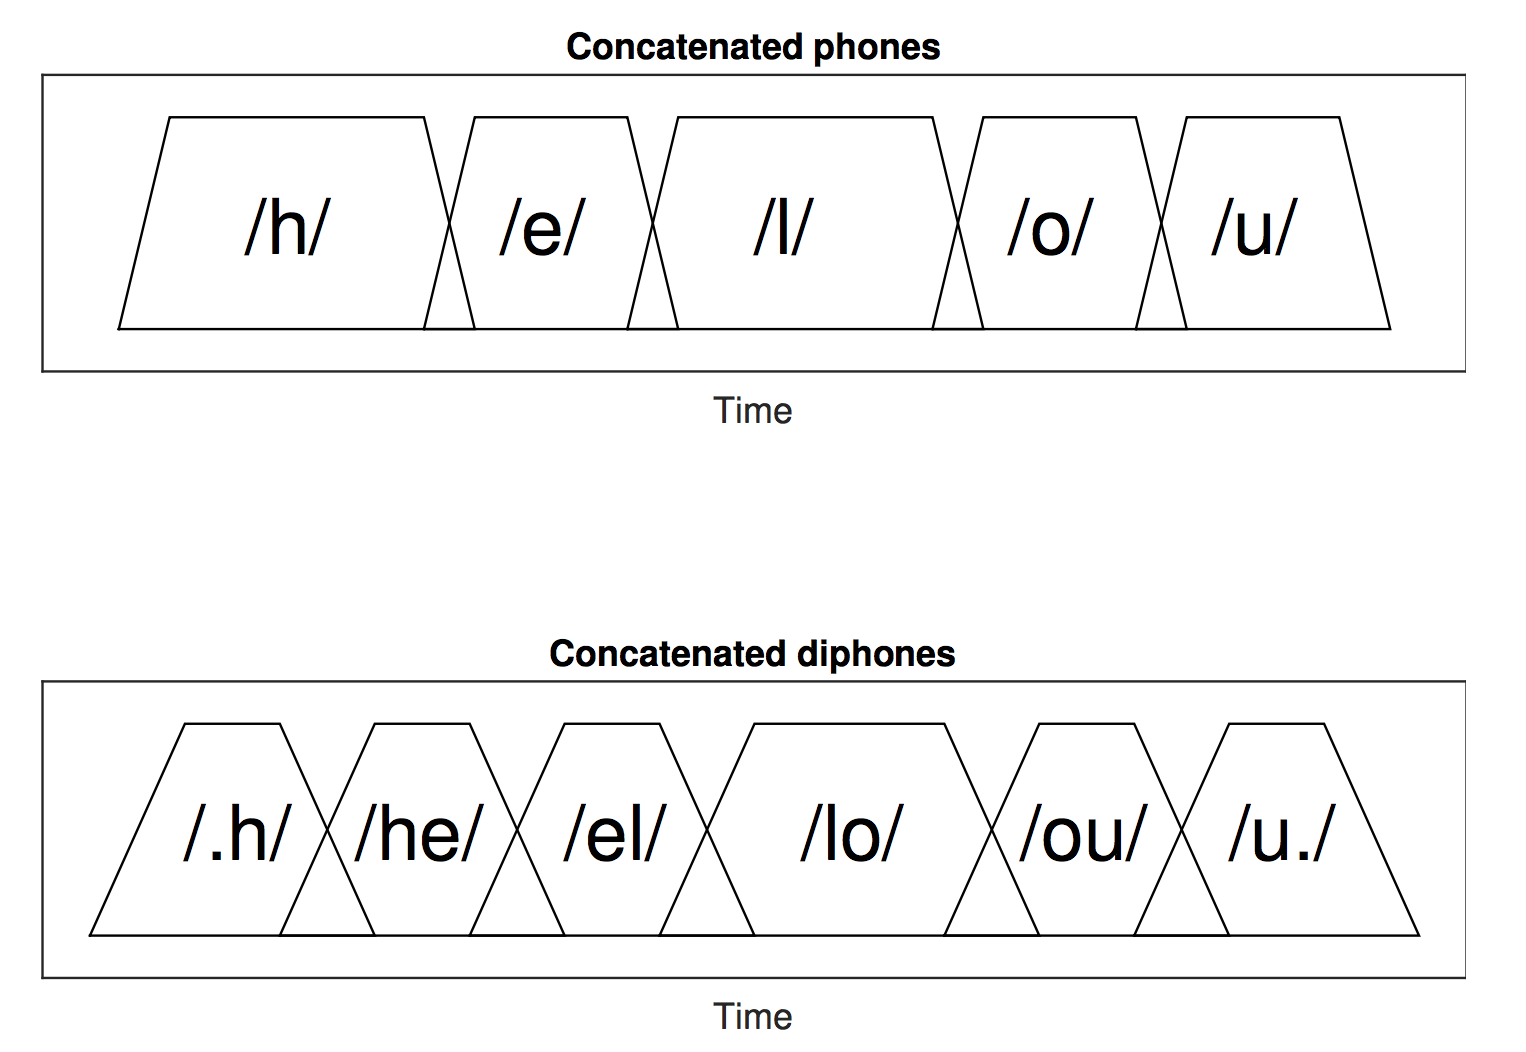
\includegraphics[width=0.7\linewidth]{img/concatenative_tts.png}
  \caption[Speech synthesis from units in concatenative TTS.]{Speech synthesis from units in concatenative TTS. (Credit: Tom Bäckström, Speech Synthesis Overview\protect\footnotemark)}
  \label{sota:figure:concatenative_tts}
\end{figure}

\footnotetext{\url{https://mycourses.aalto.fi}}

%parametric TTS
In contrast to having a large codebook, parametric TTS relies on statistical methods by generating speech with a combination of parameters like F0 and energy, modelling the human speech production \citep{Zen:2009:RSP:1576860.1577027}. Figure \ref{sota:figure:tts} illustrates the workflow of a parametric TTS system. First, morphemes in the input text are converted to phonemes through a linguistic analysis. Next, features like cepstra, F0, duration and break are calculated to be fed into the \textit{vocoder}. The vocoder finally generates the waveform using these parameters. The parameter probabilities is learned from phonetically labeled speech data and modeled as Hidden Markov Models (HMM). Recently introduced DNN-based models follow a similar approach but replace the HMM-based modelling with DNN \citep{zen_dnn}. End-to-end models, on the other hand, employ a DNN to directly synthesize speech from characters \cite{Wang2017}.

\begin{figure}[t]
  \centering
  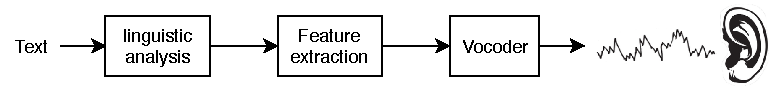
\includegraphics[width=0.9\linewidth]{img/tts_diagram.pdf}
  \caption{Basic workflow of a statistical text-to-speech system.}
  \label{sota:figure:tts}
\end{figure}

%Prosodic modelling
There exist two main parameters in evaluating a TTS system: intelligibility and naturalness. Intelligibility, as its name suggests, measures to what extend the linguistic information in a synthesized speech waveform can be comprehended. Naturalness, on the other hand, deals more with the way how an utterance is said and measures roughly the likelihood that it was said by a person and not a machine \citep{naturalness}. Naturalness is almost directly related to the prosody production in a TTS system. Prosody modelling in a TTS is predicted in three dimensions which are intonation, duration and breaks. Among a few theories on intonation modelling are the \textit{Fujisaki model} \citep{Fujisaki1983}, \textit{Tilt model} \citep{tilt}, \textit{Bezier polynomial coefficients} \citep{Escudero2002}, and \textit{Tones and Break Indices (ToBI)} \citep{tobi, Pierrehumbert}. Duration modelling deals with the prediction of segment (phone or syllable) lengths in speech. Breaks also have an important role in achieving naturalness in speech as it helps structure the discourse and also occur naturally from respiration. They can be manifested in two ways: silent, or filled, i.e.~through lengthenings or filler words \citep{zellner}. Several approaches exist for break prediction in TTS. Some recent works include \cite{DBLP:journals/pdln/AgueroB03} which models disfluency in synthesized speech through filled pauses to mimic a talking-style speech opposed to the a reading-style. \cite{DBLP:conf/iberspeech/PascualB16} focuses on silent break detection by employing RNNs. 

\subsubsection*{External Prosodic Encoding to TTS}

Some implementations of TTS systems allow the taking of external labels to influence the prosodic parameter selection process. This is performed through an interface called \textit{markup language} which accompanies the text input and conditions the sythesized speech on various acoustic/prosodic aspects. One well-known implementation of this interface is \textit{Speech Synthesis Markup Language (SSML)} \citep{ssml}. An example of an input segment to a state-of-the-art TTS system\footnote{\textit{IBM Watson TTS}: \url{https://text-to-speech-demo.ng.bluemix.net/}} that utilizes SSML tags is given below.

\begin{lstlisting}
<p><s>Conscious of its spiritual and moral heritage <break time="300ms"/>, the Union is founded on the indivisible, universal values of <prosody rate="-15%">human dignity, freedom, equality and solidarity.</prosody> It is based on the principles of democracy and the rule of law <break time="500ms"/>. </s> <s> It places the individual at the heart of its activities, <prosody rate="+15%">by establishing the citizenship of the Union</prosody> and by creating an area of freedom, security and justice.</s></p>
\end{lstlisting}


The synthesis is indicated on where to break for how long using the tag \textit{break} and tuned to speak faster or slower with the tag \textit{rate}. Usually, tags that are related with pitch, speech rate and volume are set with relative percentages and have an estimated effect on the outcome instead of an absolute effect. 

\subsection{Speech-to-Speech Translation}
\label{sota:s2s}

\begin{figure}[t]
  \centering
  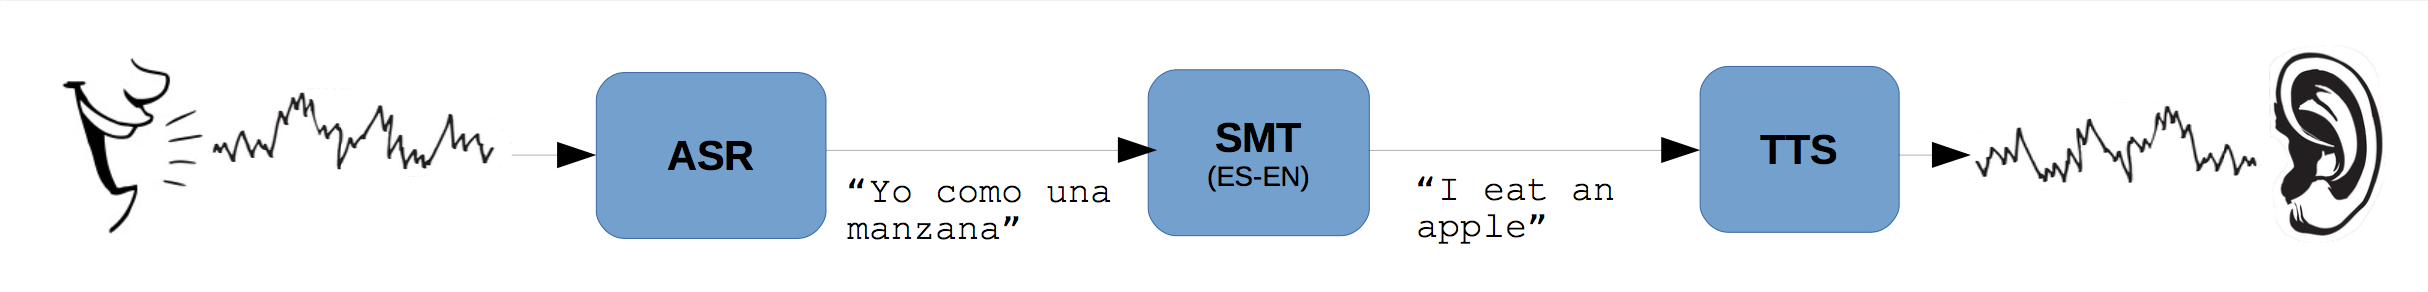
\includegraphics[width=\linewidth]{img/s2s_classic_pipeline.png}
  \caption{A conventional speech-to-speech translation pipeline.}
  \label{sota:s2s_classic}
\end{figure}

Speech-to-speech (S2S) translation enables human-to-human communication where each of the agents involved speaks in a different language. A device capable of enabling such a communication is able to accept spoken input in language A, translate it to language B and then synthesize it for hearing. By performing this process in both ways, it acts as an interface for a turn-based inter-lingual communication. Conceptually, such a system is the concatenation of the three following processes: (1) ASR, (2) MT, and (3) TTS. A diagram of the one-way process in S2S translation is illustrated in Figure \ref{sota:s2s_classic}. 

There exist various examples of S2S translation solutions resulting from both academic and commercial research. \textit{Verbmobil} is considered as the pioneer in the field as it is the oldest and most extensive research project dealing with S2S translation \citep{wahlster2013verbmobil}. It was designed for translation of spontaneous dialogues in mobile situations for the languages English, German and Japanese. \textit{IBM MASTOR} was developed in a defense oriented framework for facilitating spoken communication in low-resource languages \citep{ibm_mastor}. European Union funded project \textit{TC-STAR} was the first that addressed S2S translation in an unrestricted domain between languages English, Chinese and Spanish \citep{tcstar}. Its local counterpart \textit{TECNOPARLA} was developed with the motivation of spoken translation in the broadcast radio and television domain for the languages Catalan, English and Spanish \citep{tecnoparla}. \textit{EMIME} project was the first work that aimed voice personalization through S2S translation, where synthesized voice is adapted to sound like the recognized voice \citep{emimeemime}. Two projects with Swiss origin, \textit{SP2 SCOPES} \citep{sp2} and \textit{SIWIS} \citep{Garner:199815} that focus on Swiss and Eastern European languages report cross-lingual prosodic transfer as their main objectives. Although, there are no recorded results on the accomplishment of these objectives. 

\subsubsection{Spoken Parallel Corpora}

\begin{table*}[ht]
\begin{center}
\begin{tabular}{>{\arraybackslash} m{0.42\linewidth} >{\arraybackslash} m{0.21\linewidth} >{\arraybackslash} m{0.3\linewidth}}
\bf Corpus & \bf Languages & \bf Speech style \\ \toprule
EPIC                                            & en/it/es              & spontaneous/interpreted   \\
TC-STAR                                         & en/es, en/zh          & spontaneous/interpreted   \\
MSLT                                            & en/fr/de              & constrained \\
EMIME                                           & fi/en, de/en          & prompted                  \\
EMIME Mandarin                                  & zh/en                & prompted                  \\
SP2-Speech-Corpus                               & en/fr/de/hu/mk/sr     & prompted w/ emphasis    \\
Japanese-English emphasis                       & ja/en                & prompted w/ emphasis    \\
SIWIS database                                  & en/fr/de/it           & prompted w/ emphasis    \\
MDA~\citep{almeman2013multi}                    & 4 Arab dialects  & prompted                  \\
Farsi-English~\citep{Melvin2004CreationOA}      & fa/en                 & read/semi-spontaneous     \\
\bottomrule
\end{tabular}
\end{center}
\caption{\label{sota:corpora} A selection of available parallel speech corpora for use in S2S translation. }
\end{table*}

%Why spoken parallel corpora needed intro
The availability of large parallel corpora is one of the major challenges in developing machine translation systems. Bilingual corpora, which are needed to train statistical translation models, are harder to acquire than monolingual corpora since they presuppose the implication of labour in translation or interpretation. Working on the speech domain introduces even more difficulties since interpretations are not sufficient in capturing the paralinguistic aspects of speech. The profession of interpretation aims rapid spoken translation of speeches in e.g.~conferences, diplomatic gatherings and do not give any attention to the re-enacting of any paralinguistic features. In contrast, dubbing also covers for this aspect since the aim is to have translated voice segments of a movie or series that match with the context and lip movements in the original language. Although this domain could be rich for obtaining expressive parallel corpora, it has not been explored in any previous work. In Chapter \ref{chapter:corpusWorks}, I will explain my work in detail dealing with this type of domain \citep{bucc, Oktem2018}.

Several attempts have been made to compile large spoken parallel corpora from interpreted or fully-prompted material. Some of these corpora that were published in literature are listed in Table~\ref{sota:corpora}. Each of them show some differences in terms of its source and the way translation was handled. The EPIC corpus has been compiled from speeches from the European Parliament and their interpretations \citep{bendazzoli2005approach}. The 1 hour voice conversion corpus collected within the TC-STAR project also contains speech segments from the European Parliament and their interpreted versions in Chinese and Spanish \citep{tcstar_corpora}. The EMIME database is a compilation of prompted speeches to serve for the task of speaker conversion \citep{wester2010emime}. The MSLT corpus has been collected in bilingual conversation settings, but `there is no one-to-one alignment between sentences in the different languages as they are lightly guided conversations \citep{federmann2016microsoft}. There is a number of corpora collected for projects focusing on the emphasis translation task: SP2 Speech Corpus \citep{sevcujski2016design}, SIWIS database \citep{siwis_db} and the database collected by \cite{quoc_corpus}. These corpora contain sentence recordings with acted emphasis on the same word or word groups in both languages. 

\section{Speech Prosody Overview}
\label{sota:prosody}
In this section I will try to break down prosody to get an overview on its role in speech and also its characteristics. According to the definition by \cite{Fujisaki97}, role of prosody in speech is to organize linguistic units into an utterance and its realization involves segmental and suprasegmental features of speech. What is referred to as segmentals in this expression are the phonemes, syllables and words that have distinct boundaries in the utterance. On the other hand, suprasegmentals refers to the elements that can span over or partially cover segments in speech \citep{palmer}. Suprasegmental features in speech are the following prosodic elements: intonation, rhythm and stress. These features can be briefly explained as:

\begin{itemize}
    \item \textbf{Intonation} deals with the melodic aspects of the speech, and is realized by pitch movements. Pitch is what is perceived through the fundamental frequency (F0) involved in an audio signal. 
    \item \textbf{Rhythm} deals with the timing of phonemes, syllables and pauses in speech. Speech rate, which gives the number of segments uttered in a unit of time, is also a feature derived from rhythm.
    \item \textbf{Stress} deals with the energy in speech and is perceived through the speech signal amplitude. 
\end{itemize}

Figure \ref{sota:figure:prosodicfeatures} shows visualization of a short speech segment on Praat where pitch contour and intensity can be visualized over word and phoneme segments.  

Prosodic features are employed in speech in a complex manner to convey linguistic, para-linguistic and non-linguistic information \citep{Fujisaki97}. I will try to demonstrate the uses of these features on some examples in English. 

Intonation is considered as one of the key features in conveying attitude in many languages \citep{Prieto}. Prieto gives the simple sentence \textit{``I am cold.''} as an example for this. With different intonation structures this sentence could have many different meanings including contradiction, command (as a request to close the window) and surprise. Intonation can also be used to mark modality in sentences.  Yes/no questions, for example, commonly end with a rising pitch in English. 

Stress feature is used for marking salient points in discourse or to encode givenness. Take the example \textit{``The butler killed the him.''}. A word is marked with a stress depending on which element is already mentioned and which element is new information. This type of encoding can also be defined as phrasal stress or accent.

Rhythm and pausing is relevant in forming a hierarchical organization in speech through phrasing. The example given in \cite{zellner} expresses this very well. The length of the inter-lexical pause in \textit{``a Turkish carpet salesman''} can help distinguish if the carpets or the salesman is Turkish. Audio waveforms of both versions are visualized in the Figure \ref{sota:figure:carpet}.

\begin{figure}[t]
  \centering
  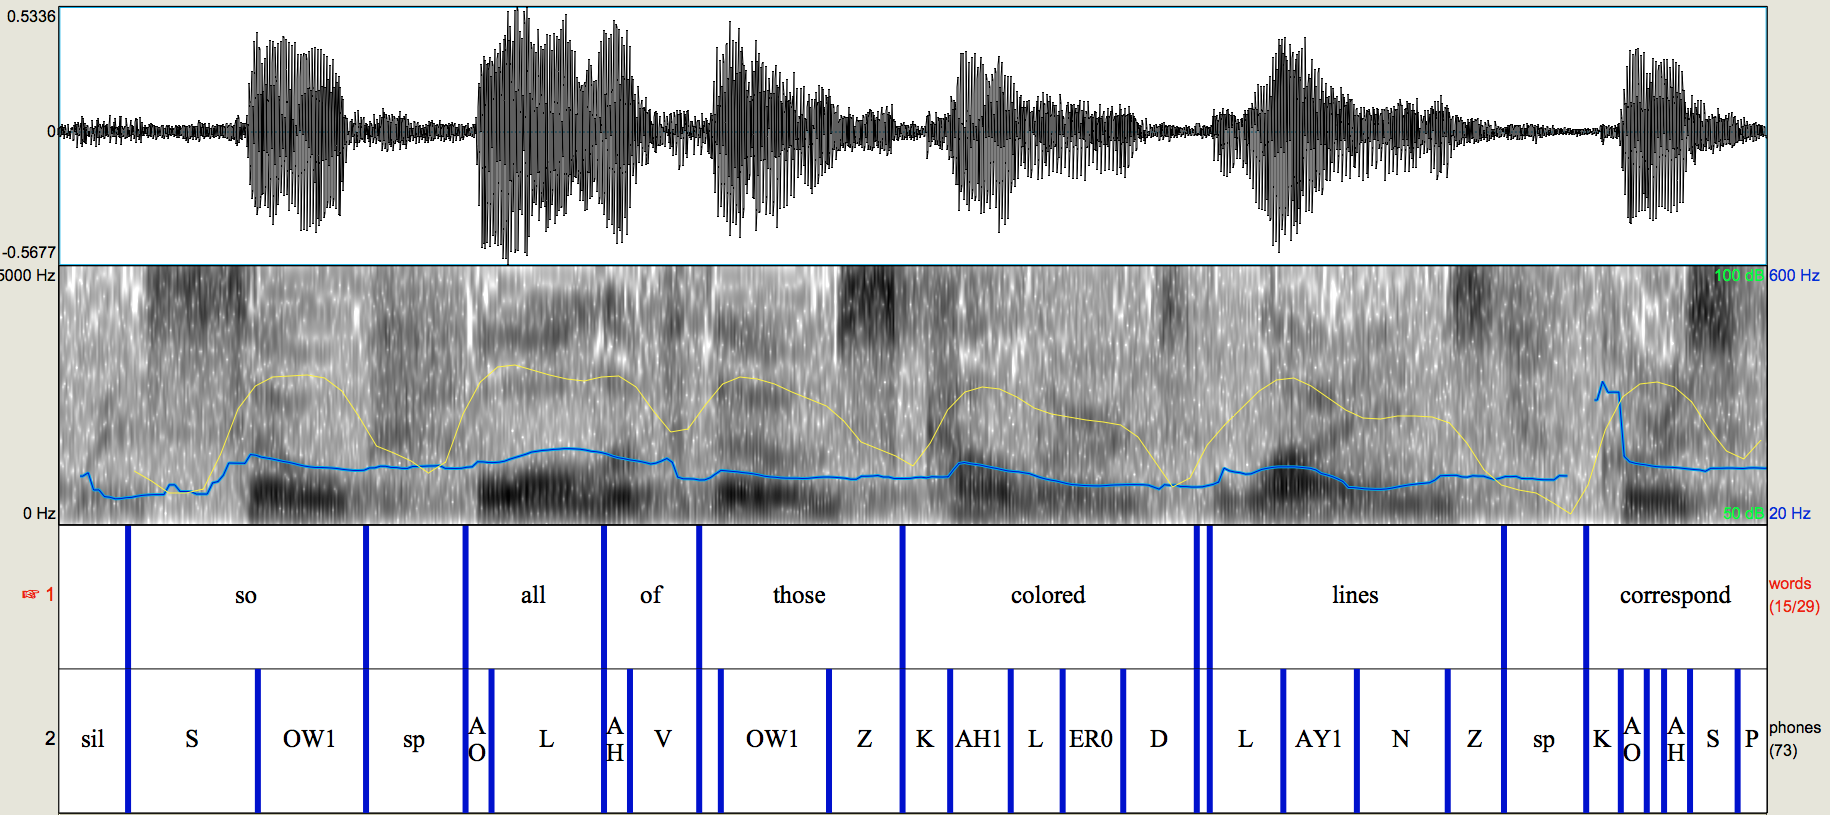
\includegraphics[width=\linewidth]{img/prosfeats_praat.png}
  \caption{Segmental (phoneme and word) and suprasegmental (pitch in blue, intensity in yellow) features of a speech signal shown with the audio waveform and frequency spectrogram. }
  \label{sota:figure:prosodicfeatures}
\end{figure}

\begin{figure}[t]
  \centering
  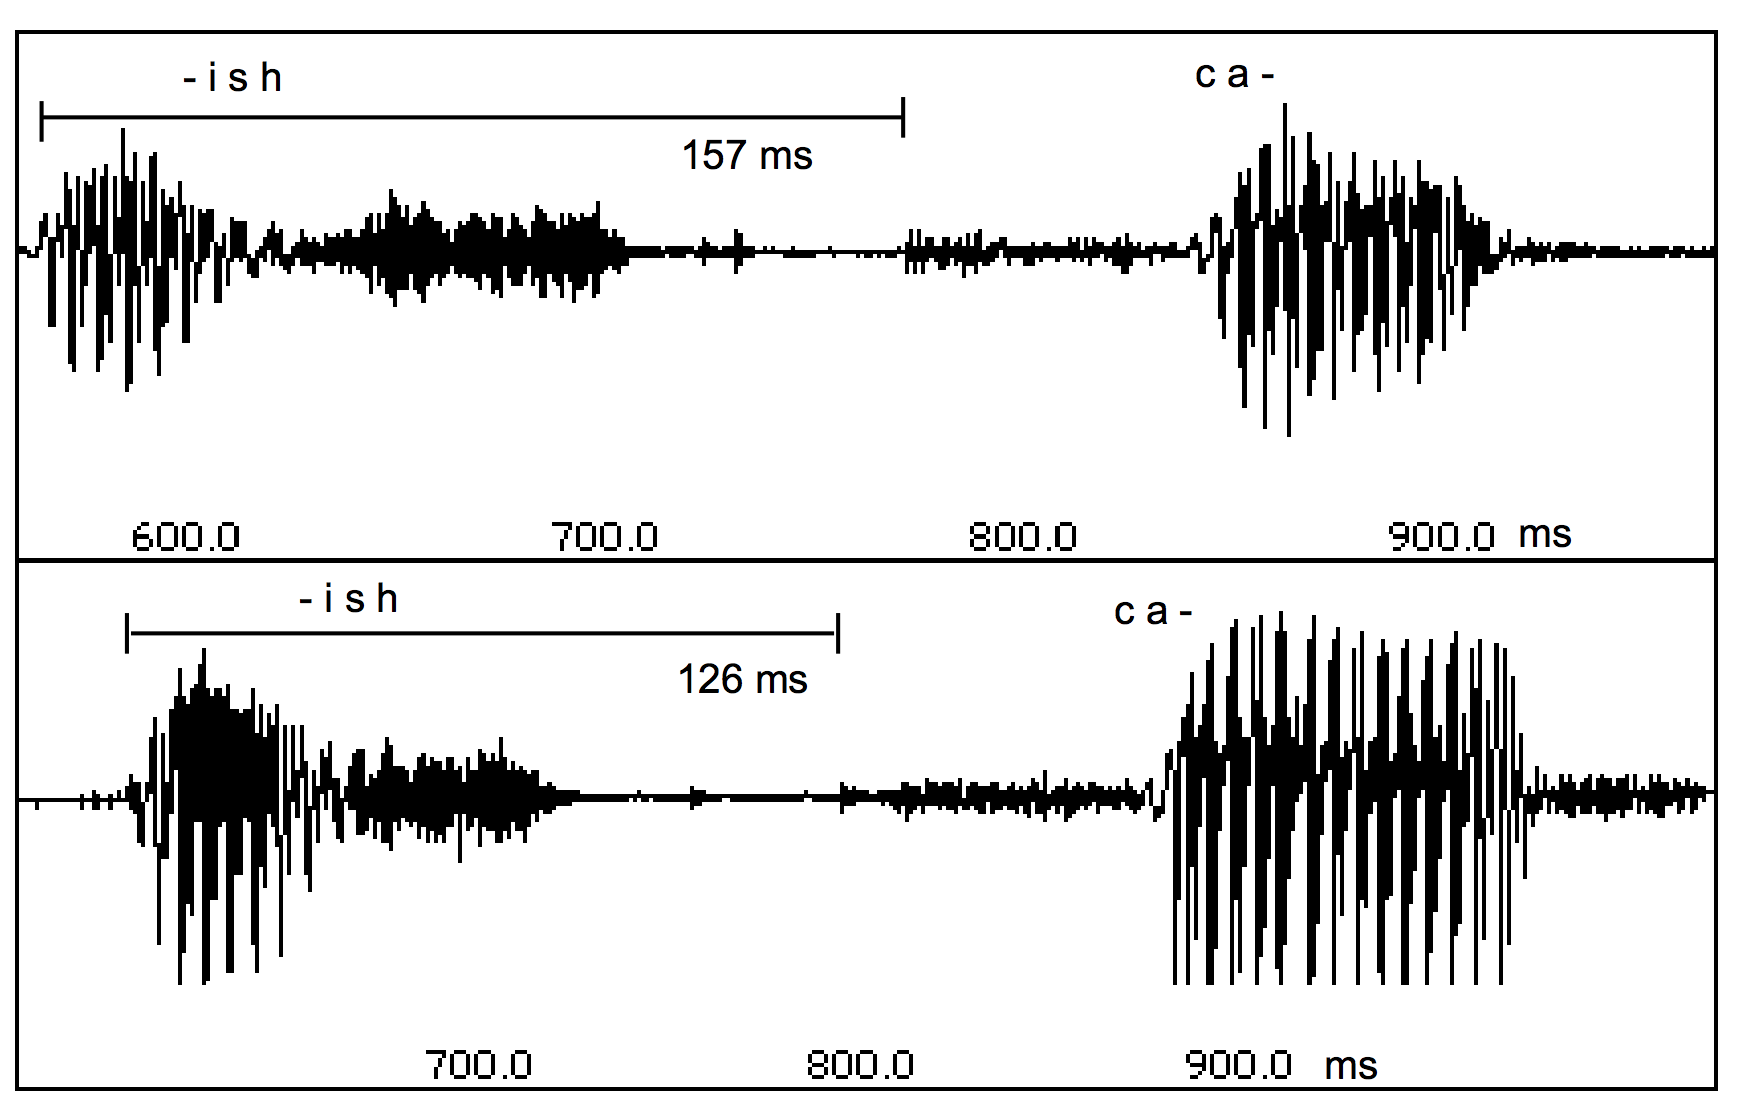
\includegraphics[width=0.8\linewidth]{img/carpet.png}
  \caption[Phrasing in speech affecting meaning.]{Phrasing in speech affecting meaning. Above ``a Turkish (carpet salesman)'', below ``a (Turkish carpet) salesman''. (Example and figure taken from \cite{zellner})}
  \label{sota:figure:carpet}
\end{figure}

It has to be noted that use of prosodic elements vary greatly between languages. In tonal languages like Chinese, Somali or Thai, it is used for encoding different semantics of words. In intonational languages like Spanish and Catalan, position of the word accent also can infer different meanings. 

Prosody is also realized in the para-linguistics of speech such as emotional state and attitude. These features however, tend to show more variety between different languages, cultures and classes \citep{cowie}. 


\section{Prosody in Speech Processing}
In Section \ref{sota:neuralspeech} I gave a review of the systems where spoken language is being processed to serve for a certain purpose. However, in these systems, speech is considered only with the linguistic content (i.e. words, phrases, etc.) it carries. Prosodic features that are encoded through various acoustic phenomena like intonation, energy, breaks etc. are disregarded in any further analysis.  

In this section, I will review recent as well as some historical works that regard prosody as an essential dimension in a speech processing framework. These works not only argue that prosodic features in spoken language are important for spoken language applications, but also suggest methodologies for their inclusion and report progress through it. 

I will present two applied areas where prosodic cues are utilized as an advancement for speech processing systems. First, in automated speech transcription where prosodic cues are used for phrase boundary detection or punctuation restoration, then in speech-to-speech translation where a complete linguistic and paralinguistic information transfer is desired.

\subsection{Utilizing Prosody in Punctuation Restoration in Transcribed Speech}
\label{sota:punk_prosody}
It has been shown that prosodic features are highly indicative of phrase boundaries as well as of punctuation placement in many works \citep{punctuation_book}. Therefore, a great deal of effort has been put in several works into the use of prosodic features in punctuation restoration when original speech is available. In \cite{levy2012effect}, the authors successfully detect automatically full stops in ASR output with no language modeling using only weighted pause, F0 changes and amplitude range values. Commas are shown to be more difficult to detect when only prosodic features are used. In \cite{baron2002automatic}, it is demonstrated that combination of language and prosodic models performs better than single-model approaches. 

Many studies consider punctuation restoration as a problem of determining the probability of a certain label at a boundary point in speech, e.g. between words or at pauses, calculated in the vicinity of that point. Prosodic and textual cues around each inter-word boundary are taken as features for a decision tree classifier to detect sentence boundaries in \cite{liu2006study}. Similarly in \cite{khomitsevich2015combining}, word and grammatical n-gram features are combined with prosodic features to detect punctuation marks in Russian ASR system. \cite{Psutka04automaticpunctuation} focus on Czech broadcast news speech to detect commas and sentence boundaries by using a prosodic model based on decision trees and language model based on n-grams. 

A combination of lexical-, prosodic-, and speaker-based features is also found in \cite{batista2012bilingual} for the detection of full stops, commas, and question marks in a bilingual English-Portuguese broadcast news corpus. Similar works deal with the punctuation generation problem by using statistical models of prosodic features \citep{Christensen01punctuationannotation}, the combination of both textual and prosodic features based on adaptive boosting \citep{kolar2012development}, and a cross-linguistic study of prosodic features through two different approaches for feature selection: a forward search wrapper and feature filtering \citep{fung2007cross}. Also, in \cite{Klejch}, frame-level prosodic features (only pitch and pause) are integrated in a neural machine translation based system with a hierarchical encoder.

Combining lexical and prosodic models has been employed in a bidirectional neural network setting in \cite{Xu2017} for sentence boundary detection and in \cite{tilk2016bidirectional} for punctuation restoration. Both approaches are based on training of the language model (on large amounts of textual data) separately to the acoustic model (from a smaller corpus), eventually leading the models to bias on written data. 

\subsection{Utilizing Prosody in Spoken Language Machine Translation}
\label{sota:prosody_in_smt}

% Utilization prosody is relevant in SLMT in three ways: (1) for segmenting input into sentence-like units (2) for  it can be helpful in resolving ambiguous translations and (2) it is worth to carry prosodic features to the target synthesis on a S2S translation setup. 

% The example given earlier from \cite{zellner} is helpful in demonstrating the use of prosody in a spoken language input translation system. The phrase ``Turkish carpet salesman'' could be translated in two ways to Spanish: either ``vendedor turco de alfombras'' or ``vendedor de alfombras turcas''. This disambiguation is only possible through the perception of the break and intonational structure in the sentence. 

%intro
There has been considerable work on inclusion of prosody into speech-to-speech translation pipelines. Most of the research based systems give some of the focus onto this area as it is believed that spoken translation is truly complete only through conveying of prosody as well as linguistic information between source and target phrases. On another aspect, some research focus on the fact that ASR output is not optimized to be inputted to machine translation. ASR outputs only a raw sequence of words without any further information on sentence or phrase boundaries and thus harms MT quality that necessitates a certain input size and context. 

It is observed that there are three main objectives when it comes to incorporation of prosody into a S2S framework. These objectives are: (1) segmentation of the source phrase into meaningful units through use of prosody to aid the machine translation step, (2) transfer of prominence (emphasis) in input speech into the synthesized translations and (3) using context information to boost translation accuracy. 

%first use verbmobil (2000)
First use of prosody within a spoken language translation system was within the \textit{Verbmobil} project \citep{verbmobil_prosody}. A group of prosodic features were computed for the word hypotheses computed by the ASR module. These were: probabilities for clause boundaries, accentuation and sentence mood. Among these, a major improvement was achieved through the classification of clause boundaries in the input phrases. Syntactic parsing of the recognized words was improved in terms of readings and computation time only through the segmentation of the input phrases. Boundary classification was based on a combination of textual and prosodic features (energy, duration and F0). A similar approach is investigated in \cite{Matusov07improvingspeech}. A lexical-prosodic boundary prediction algorithm is introduced and compared with various other segmentation algorithms in terms of their effect on translation quality. They show that translation is optimized through usage of a boundary prediction algorithm based on prosodic features and phrase probabilities using a language model. 

%aguero, adell, bonafonte
\cite{aguero2006prosody} can be considered as the first example where objective is to transfer the underlying paralinguistic features in the source speech to the synthesized target speech. The methodology they present aims to find transfer patterns of F0 contours in source and target speech in a S2S framework. This is done with an extension on the intonation prediction module of the TTS that does not only consider linguistic features of the target translation but also features derived from the source speech. The intonation patterns of phrases of the input sentence is first classified and then mapped into intonation patterns of the target language. These transformations are learned from a bilingual corpus and integrated as an enhancement to a phrase-based translation system. They report improvement over preferences of the synthesized translations in terms of naturalness. 

%CSU
A similar approach is followed in \cite{anumanchipalli:2012} for word-level emphasis transfer. They explain their motivation with experimentation on a subset of the bilingual speech corpus they collected. By manual inspection, they see that there's a match of 48\% of the emphasized words in the parallel languages. Their cross-lingual intonation transformation methodology is based on learning the mapping between word-level intonation contour parametrizations between two languages from a single-speaker bilingual dataset. Since they do not perform the machine translation itself, they are able to compare intonation contours generated in a neutral way and with their enhancement. They show that through this process generated contours get closer to the reference contours in their dataset.

%TODO: \mireia{Here I miss some more recent works on emphasis transferring that we found last year, like Honnet's thesis: \footnote{http://publications.idiap.ch/downloads/papers/2017/Honnet_THESIS_2017.pdf} %http://publications.idiap.ch/downloads/papers/2017/Honnet_THESIS_2017.pdf}

Do et al.~approach cross-lingual prosodic transfer from a perspective based on transferring of word-level emphasis. Their general approach is to label each word in the source token sequence with a real-numbered emphasis level and then map it into the words in target sequence using a transformation function. Emphasis modelling is performed with linear-regression hidden-semi Markov models (LR-HSMMs) that is trained on F0, duration and energy features \citep{Quoc2016}. Their methodology for mapping input emphasis estimations to target emphasis weights show change over various works. In \cite{Quoc2016}, this is performed using a model based on conditional random fields (CRFs) (Figure \ref{sota:quoc}a). Following, in \cite{Quoc2016b}, they utilize a LSTM based model with attention that exploits the word alignment information of machine translation. They record an improvement of 1\% in terms of emphasis prediction F-measure (Figure \ref{sota:quoc}b). Both of these approaches incorporate prosodic transfer process as an additional module besides MT and assume perfect translations. This is later addressed in \cite{Quoc2017} and \cite{Quoc2018} where emphasis and word prediction are done jointly within a sequence-to-sequence MT system (Figure \ref{sota:quoc}c). The lack of parallel spoken data is covered by a two-stage training procedure. Translation model is first trained on a large text corpus and then emphasis modelling is generated from a smaller laboratory generated English-Japanese parallel corpus. Their results show that text translation does not improve with inclusion of emphasis weights. As a simpler system is introduced, gain on computational time is recorded, however, without an improvement on emphasis prediction compared to previous works. All in all, they report that their models are speaker dependent and is demonstrated on a highly controlled setting. This can be explained by the corpus they use at hand which consists of a small set of samples with acted emphasis. 

\begin{figure}
\centering
\begin{tabular}{c}
  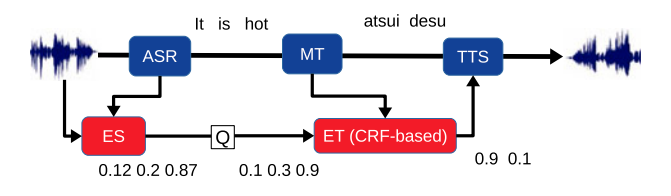
\includegraphics[width=0.7\linewidth]{img/quoc_a.png} \\
(a) CRF-based \\[6pt]
 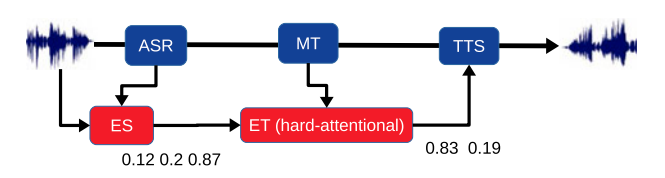
\includegraphics[width=0.7\linewidth]{img/quoc_b.png} \\
(b) Hard-attentional \\[6pt]
 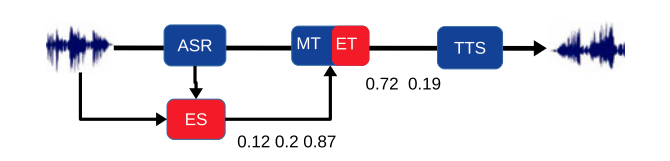
\includegraphics[width=0.7\linewidth]{img/quoc_c.png} \\
(c) Joint model \\[6pt]
\end{tabular}
\caption[Various implementations of S2S translation systems with emphasis transfer.]{Various implementations of S2S translation systems with emphasis transfer. (Diagrams are taken from \cite{Quoc2018}) }
\label{sota:quoc}
\end{figure}

%pause transfer
Pausing in speech is an important prosodic feature that affects both emphasis perception and phrasing. Transfer of pauses within S2S translation is addressed in the works: \cite{truong2015_iwslt} and \cite{bonafonte:pausetransfer}. In the former one, pause prediction is incorporated into the CRF-based emphasis prediction module and shows improvement in terms of emphasis perception in the synthesized examples. The latter work focuses on the transfer of the phrasing and follows a rule-based approach exploiting alignment information from SMT. 

%context enrichment
Some work on use of prosody in S2S translation focuses on employing prosodic features available through acoustic or linguistic analysis to further boost translation accuracy. These works are mostly inspired from approaches where factored SMT is enhanced with linguistic features (e.g.~POS features) and employ a similar approach in spoken translation. \cite{Guo2016} is an example where additional prosodic features based on pronunciation, boundary marks and emphasis is integrated as factors to a factored translation model based system. They record slight improvement in terms of translation accuracy with inclusion of boundary marks when translated from Chinese to English. In the opposite direction, they record improvement with inclusion of all three features. Again in \cite{RangarajanSridhar:2013:enrichingS2S}, factored translation models used for phrase-based translation is extended to accept additional prosodic information on source and target sides. They test inclusion of dialog information such as question types in source side and pitch accent based prominence features on the target side. Modest improvements are recorded in terms of translation accuracy. 

Having reviewed the fundamental concepts and state-of-the-art, I will move in next section on presenting the corpus related work. 
\newpage\leavevmode\thispagestyle{empty}\newpage
% ---------------------------------------------------------------------

% CHAPTER 3: Corpus works
% ---------------------------------------------------------------------
%**************** Bilingual corpus building **************
\chapter{Compiling corpora for building data-driven prosodic models}
\label{chapter:corpusWorks}

In order to develop data-driven models related to speech prosody, one needs access to a sufficient number of speech samples that are annotated with prosodic features. Spoken samples collected to form a corpus serve for developing models for machine-learning applications as well as empirical research. A prosodically annotated spoken corpora usually consists of speech samples, their transcriptions and certain acoustic and prosodic labels associated with it. There is a few number of publicly available speech corpora that serve for prosody research as it is hard to process and annotate \citep{rosenberg}. One major work that this dissertation involves is collection of corpora to develop prosodic models on spoken language applications. This chapter presents: two prosodically annotated corpora that were used during this work, methodologies followed in compiling them and also further tools that were used and developed during the process.

There are two different methods for compiling spoken language corpora. First approach involves recording of designated speakers reading prepared text material in a controlled environment. Although this approach is the best way to obtain noiseless data, it is very expensive and hard to re-scale. Moreover, it poses a further disadvantage if prosody is an important aspect. As speakers are placed in a controlled environment their speech lacks the prosodic features that would normally be present in a more natural setting. 

Another approach to corpus development lies in exploiting readily available recorded media material such as conference talks, TV shows or movies. \mireia{TODO:[The concept of "found data" is used in theses cases. \footnote{See e.g. http://tts.speech.cs.cmu.edu/pbaljeka/www/Thesis\_Final.pdf}]}This kind of data source is more prone to noise and necessitates various automated and manual processing methodologies to shape it to the need of the application need. However, two big advantages that this method gives are that (1) the speakers can have more naturally expressive prosody, and (2) relatively low-cost scalability that comes with development of automated extraction methods. 

For the sake of obtaining data to be used in the methodologies presented in this dissertation, automated approaches that exploit readily recorded material were followed \cite{bucc, Oktem2018}. Two main sources of spoken data have taken advantage of: conference talks and subtitled movies and TV shows. The methodologies developed to process this material were compiled as open-source software libraries accessible online\footnote{\url{www.github.com/alpoktem}} (Sections \ref{corpusWorks:toolkit} and \ref{corpusWorks:movie2parallelDB}). Two corpora were obtained through the result of these processes: First one is the re-compiled and published \textit{TED talks corpus}, which is modified from \cite{Farrus:SP:2016} to suit experiments related to prosodic punctuation recovery task (Section \ref{corpusWorks:ted}). Second is the \textit{Heroes corpus}, which consists of parallel English and Spanish speech segments gathered from a TV series to suit prosodic translation task (Section \ref{corpusWorks:heroes}). Both of these corpora are made accessible openly through UPF Digital Repository: \url{repositori.upf.edu}. 

Another task as important as obtaining of prosodically annotated corpora is analyzing them in terms of various prosodic features. The nature of prosodic data introduces its challenges and thus necessitates specialized tools to accommodate its analysis. In this chapter, I will also present \textit{Prosograph}, which helps analyze data of this type in a simple and clear way (Section \ref{corpusWorks:prosograph}). 

\section{Toolkit for Prosodically Annotated Speech Data Creation}
\label{corpusWorks:toolkit}

In this section, I will introduce some of the principal tools employed that served an important role in the presented corpus development processes. 

\subsection*{\textit{Proscript} for Prosodic Data Handling}
%Introduce the problem and need
Handling speech data together with prosodic annotations introduces its own challenges. Prosody can be seen as a phenomena parallel to the words uttered in speech. In its essence, written representation of speech only is only sufficient in representing a limited dimension of it through orthographic symbols. There has been work to represent aspects of prosody together with the written form of speech (orthography). For example, ToBI convention introduced in \cite{tobi} represents speech prosody in 4 tiers. These four tiers are agreed annotation styles for representing intonation, accents and breaks in correspondence with utterance. 

Computational applications that deal with prosody necessitate a standard in digitally representing the structure of speech with its orthography and prosody together. One of the most popular of these conventions is the \textit{TextGrid} file format, which is used by \textit{Praat} \citep{boersma01}. This XML based file format stores any number of tiers that can be used to label prosodic features. Although very useful for visualization in Praat, this format is not designed to be functional for viewing and manipulating for itself. Every tier defines which event occurs at what time on its own and it is difficult to associate events that occur in parallel in different tiers. Also, for handling raw acoustic features Praat uses different file formats. Due to this design, a complete prosodic/acoustic representation of a short utterance ends up being represented with a clutter of files.

%What is introduced?
An optimal and standard data structure was needed in this study for two reasons: for accommodating creation and storage of prosodic data and also for easy processing with machine learning applications. \textit{Proscript} framework was created to remedy for this deficit. It is both a data representation format and a specialized library for creation, manipulation, reading and writing of this sort of data. The name \textit{Proscript} is a portmanteau of the words \textit{prosody} and \textit{transcript}. It is seen as an enhanced way of representing a speech transcript. Instead of tiers, speech is represented with its features that occur in parallel at discrete bounded intervals. These bounded intervals can be words or a group of words that is called ``segments''. A segment can represent, for example, a prosodic phrase, a sentence or a group of sentences. Any type of feature can be stored within these boundaries. Be it acoustic features such as intonation, intensity or morphosyntactic features as part of speech or speaker tags. 

\begin{table}[th]
  
  \centering
  \begin{tabular}{>{\arraybackslash} m{0.25\linewidth} | >{\arraybackslash} m{0.6\linewidth} }
    \toprule
    \textbf{Feature} & \textbf{Details} \\
    \midrule
    word                         & as a token                                           \\
    id							 & unique word id				                        \\
    speaker id                   & unique speaker id                                    \\
    start time                   & start time of the word in an associated audio file   \\
    end time                     & end time of the word in an associated audio file     \\
    pause                        & coming before and after the word                     \\
    punctuation                  & coming before and after the word                     \\
    POS                          & part-of-speech                                       \\
    ToBI                         & ToBI label                                           \\
    mean f0                      & in Hertz and log-scaled (semitones)                   \\
    mean intensity               & in decibels and log-scaled                            \\
    f0 contour                   & as a list in Hertz or semitones                      \\
    intensity contour            & as a list in Hertz or log-scaled                      \\
    speech rate                  & relative to syllables \mireia{TODO: in which units?}           \\
    \bottomrule
  \end{tabular}
  \caption{Word-level information kept in an example Proscript format file.}
  \label{tab:proscript}
\end{table}

\textbf{Proscript file format} is based on the CSV file format. First line is the names of features that particular file stores and the following lines are the sequence of syntactic units together with the features that go parallel with them. See Table \ref{tab:proscript} for an example of parallel features stored in a Proscript file. In this particular example the discrete units are defined as words. The set of features is changeable. For example, a most simple set would be the words and their timing information without any syntactic or prosodic features. This set would be suitable for storing word-alignment information. 

A Proscript file can represent a short utterance as well as a whole dialog between two speakers. Dialog turns, for example, can be represented as segments with the speaker id tagged. Use is kept highly customizable through the library designed to handle Proscript files. 

\textbf{Proscript Python library} was developed in order to make creation, manipulation and annotation of Proscript files as easy as possible. It can be imported from a Python script to batch process transcripted speech files, annotate them with the desired features and output as files. Both word alignment and prosodic acoustic tagging software (explained in following subsections) is accessible through the library. 

Proscript as python package is accessible online\footnote{\url{github.com/alpoktem/proscript}}. Guide and example scripts are provided in the repository on development. A ``Proscripter'' script is provided to obtain Proscript file from a audio file and its transcription. \footnote{Proscript file format is used as the accepted format in the other frameworks (Prosograph, punkProse, transProse) introduced in this dissertation.}

\subsection*{\textit{Montreal Forced Aligner} for Speech-to-text Alignment}
%Why alignment is needed?
Speech-to-text alignment is the process of determining boundary points of words and phonemes present in speech audio recordings defined by their text transcriptions. It proves to be essential for the work in this dissertation as it helps to align prosodic features in speech within their morphologic boundaries in their transcription. 

For this task, the open-source \textit{Montreal Forced Aligner} (MFA) \citep{mfa} is employed. Forced alignment process is built on an automatic speech recognition system and requires its own acoustic models and a pronunciation dictionary. Although pre-trained models for both English and Spanish is provided through the website of the tool\footnote{\url{montreal-forced-aligner.readthedocs.io/}}, Spanish pronunciation dictionary is not openly available. For this reason, a Spanish pronunciation dictionary has been created that uses the same phoneme set as MFA\footnote{Resource available in: \url{https://github.com/TalnUPF/phonetic_lexica}}. Vocabulary has been gathered from the open source spell checker tool \textit{ISpell}\footnote{\url{https://www.gnu.org/software/ispell/}}. Phonetic transcriptions of each word in this dictionary was obtained by using \textit{TransDic} software \citep{Garrido2018}.

\subsection{\textit{ProsodyTagger} for prosodic feature annotation}
In order to augment speech data with prosodic/acoustic features \textit{ProsodyTagger} is used. \textit{ProsodyTagger} \citep{tagger} is a part of the \textit{Praat on the Web} service\footnote{\url{kristina.taln.upf.edu/praatupf}} \citep{praatontheweb} and was provided by its main author Dr. Mónica Domínguez for carrying out prosodic feature annotation task within the Proscript library. The tool is based on \textit{Praat} and simplifies the process of extracting mean f0 and intensity features in speech given its segmentations as a TextGrid file. See Figure \ref{corpusWorks:figure:pros_features} for an illustration of the prosodic features extracted for a speech utterance using this tool. 

\begin{figure}
\centering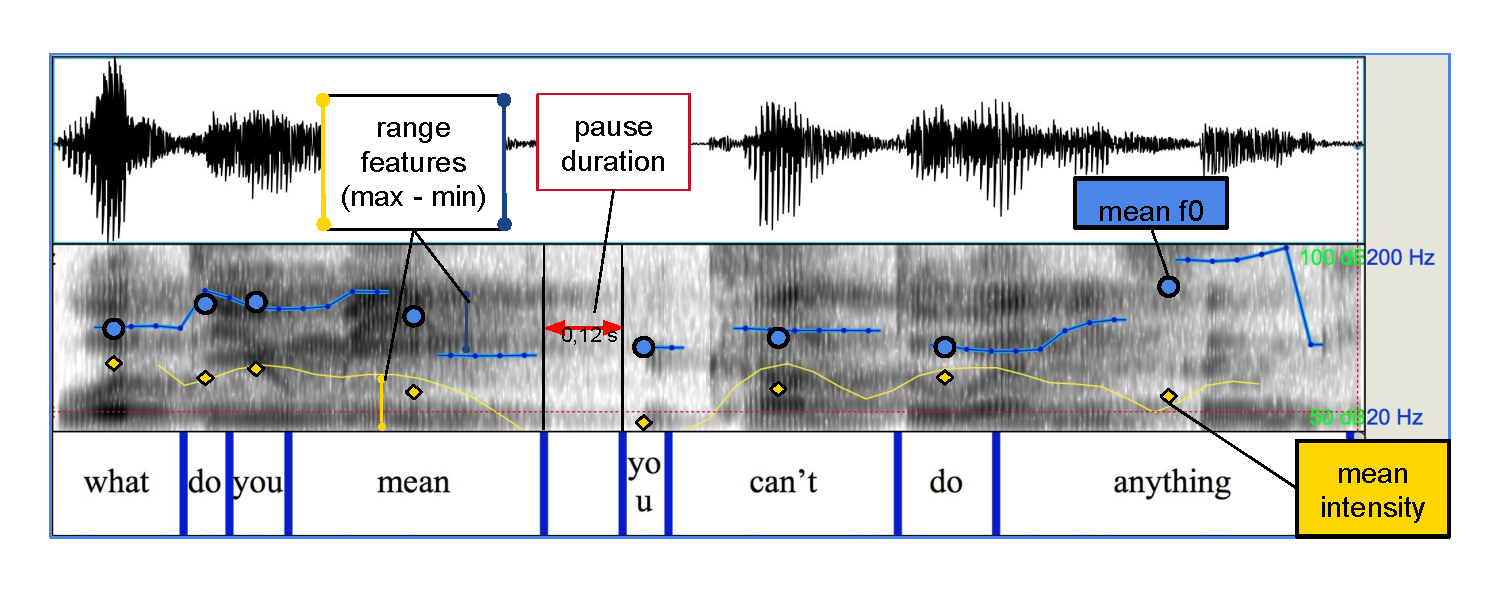
\includegraphics[width=\linewidth]{img/pros_features.pdf}
\caption{Word-level prosodic feature labelling.}
\label{corpusWorks:figure:pros_features}
\end{figure}

\section{Compiling the \textit{Prosodically Annotated TED Talks Corpus}}
\label{corpusWorks:ted}

In this section, I will introduce the TED talks corpus that was recompiled and published to serve for the automatic punctuation restoration work (explained in Chapter \ref{chapter:punkProse}). TED (Technology, Entertainment, Design) talks are a set of conference talks lasting in average 15 minutes each that have been held worldwide in more than 100 languages. They include a large variety of topics, from technology and design to science, culture and academia.  The corresponding transcripts, as well as audio and video files, are available openly on TED's website\footnote{\url{www.ted.com}}. For its public availability, TED talks have been the source of many corpora for linguistic analysis and machine learning based applications. Different formats of corpora based on TED talks cover areas from automatic speech recognition \citep{tedlium} to document classification \citep{Hermann:2014:ACLphil} and machine translation \citep{cettoloEtAl:EAMT2012}. 

\cite{Farrus:SP:2016} studies paragraph-based prosodic cues in TED talks for the aim of improving naturalness in synthesizing spoken discourse. The dataset used for this work consists of 1365 talks published before 2014. Using the punctuation and paragraph annotated transcriptions available on the website, several prosodic analyses has been performed and stored at various lengths: words, sentences, segments (from subtitles) and paragraphs. Word and sentence timings were extracted using forced alignment. Pause durations between words were extracted from the provided word timings. Acoustic annotations are done at each interval automatically using the Praat software \citep{praat:2016}. Fundamental frequency (F0) and intensity contours were extracted at 10 ms precision and then converted to semitones relative to speaker mean value. Speaker mean values were represented by zero values in both cases. 

Although available on demand, this extensive corpus is not published in an open way. Moreover, it was found out that words, word timings, punctuation information and acoustic features associated with words were scattered among many files in the corpus. This made it difficult to process and create training data for machine learning based experiments. For these reasons, the corpus was re-processed, taking the information as it is, but making it easily readable. 

Due to some talks lacking acoustic annotations, the recompiled corpus consists of a subset of 1038 talks in the original corpus. These talks were given by 877 English speakers, which means that some speakers were present in various talks. Through counting of sentence-ending punctuation marks, 155174 sentences were calculated to be present in this version. The dataset is published online as \textit{Prosodically annotated TED talks} and is accessible through \url{repositori.upf.edu/handle/10230/33981} with Attribution 4.0 International (CC BY 4.0) license\footnote{\url{https://creativecommons.org/licenses/by/4.0/}}. Source code used during the recompilation of this corpora is also provided online\footnote{\url{https://github.com/alpoktem/ted_preprocess}}.


\section{Automatic Extraction of Parallel Speech Corpora from Dubbed Movies}
\label{corpusWorks:movie2parallelDB}
Dubbing is the process of voice acting on top of the dialogues in a movie, TV series or documentary to make it accessible to viewers of another language. Popularity of dubbing of media material for a language depends greatly on the language culture of the country where the language is mainly spoken. For countries that prefer watching films on their mother-tongue, most movies and TV series go through this process before being released. Dubbing is carried out in professional studios and with professional voice actors. 

There are certain characteristics of art of dubbing that makes it an interesting candidate as a resource for parallel corpora. The process as a whole can be considered as a translation process. However, it has much more points to be heeded than just merely translating the movie script. Actor and actresses lines have to be translated in a way that the lengths of the dialogues match. This is to ensure that voice-overs match the lip movements of the original actors. Once a translation that fits a line is found, voice actors record the segment over the original movie respecting the way of acting of the original actors. It can be seen as a way of re-enactment of the line but with another language. Eventually, the voice-over doesn't only carry the content to the dubbing language but also the paralinguistic aspects that go with it. 
A methodology has been built around getting advantage of this kinds of resources to obtain parallel speech corpora. In contrast with a methodology based on collecting bilingual samples in a controlled environment, I propose to exploit dubbed movies where expressive speech is readily available in multiple languages and their corresponding aligned scripts are easily accessible through subtitles. The time information in subtitles makes it easy to align sentences of different languages since timing is correlated to the audio. 

The proposed methodology needs only raw movie data, does not require any training (as is the case of \cite{tsiartas2011bilingual}) and satisfies the following requirements: (1) it is easily expandable, (2) it supports any pair of languages where dubbed material is available, (3) it can handle any domain and speech style, and (4) it delivers a parallel spoken language corpus with annotated expressive speech. I will refer to ``Expressive speech'' as that speech that is prosodically rich, which is a feature needed in developing speech-to-speech translation applications where prosody is being taken into account. %TODO: check this sentence

\afterpage{%
    \begin{figure}[p]
      \centering
      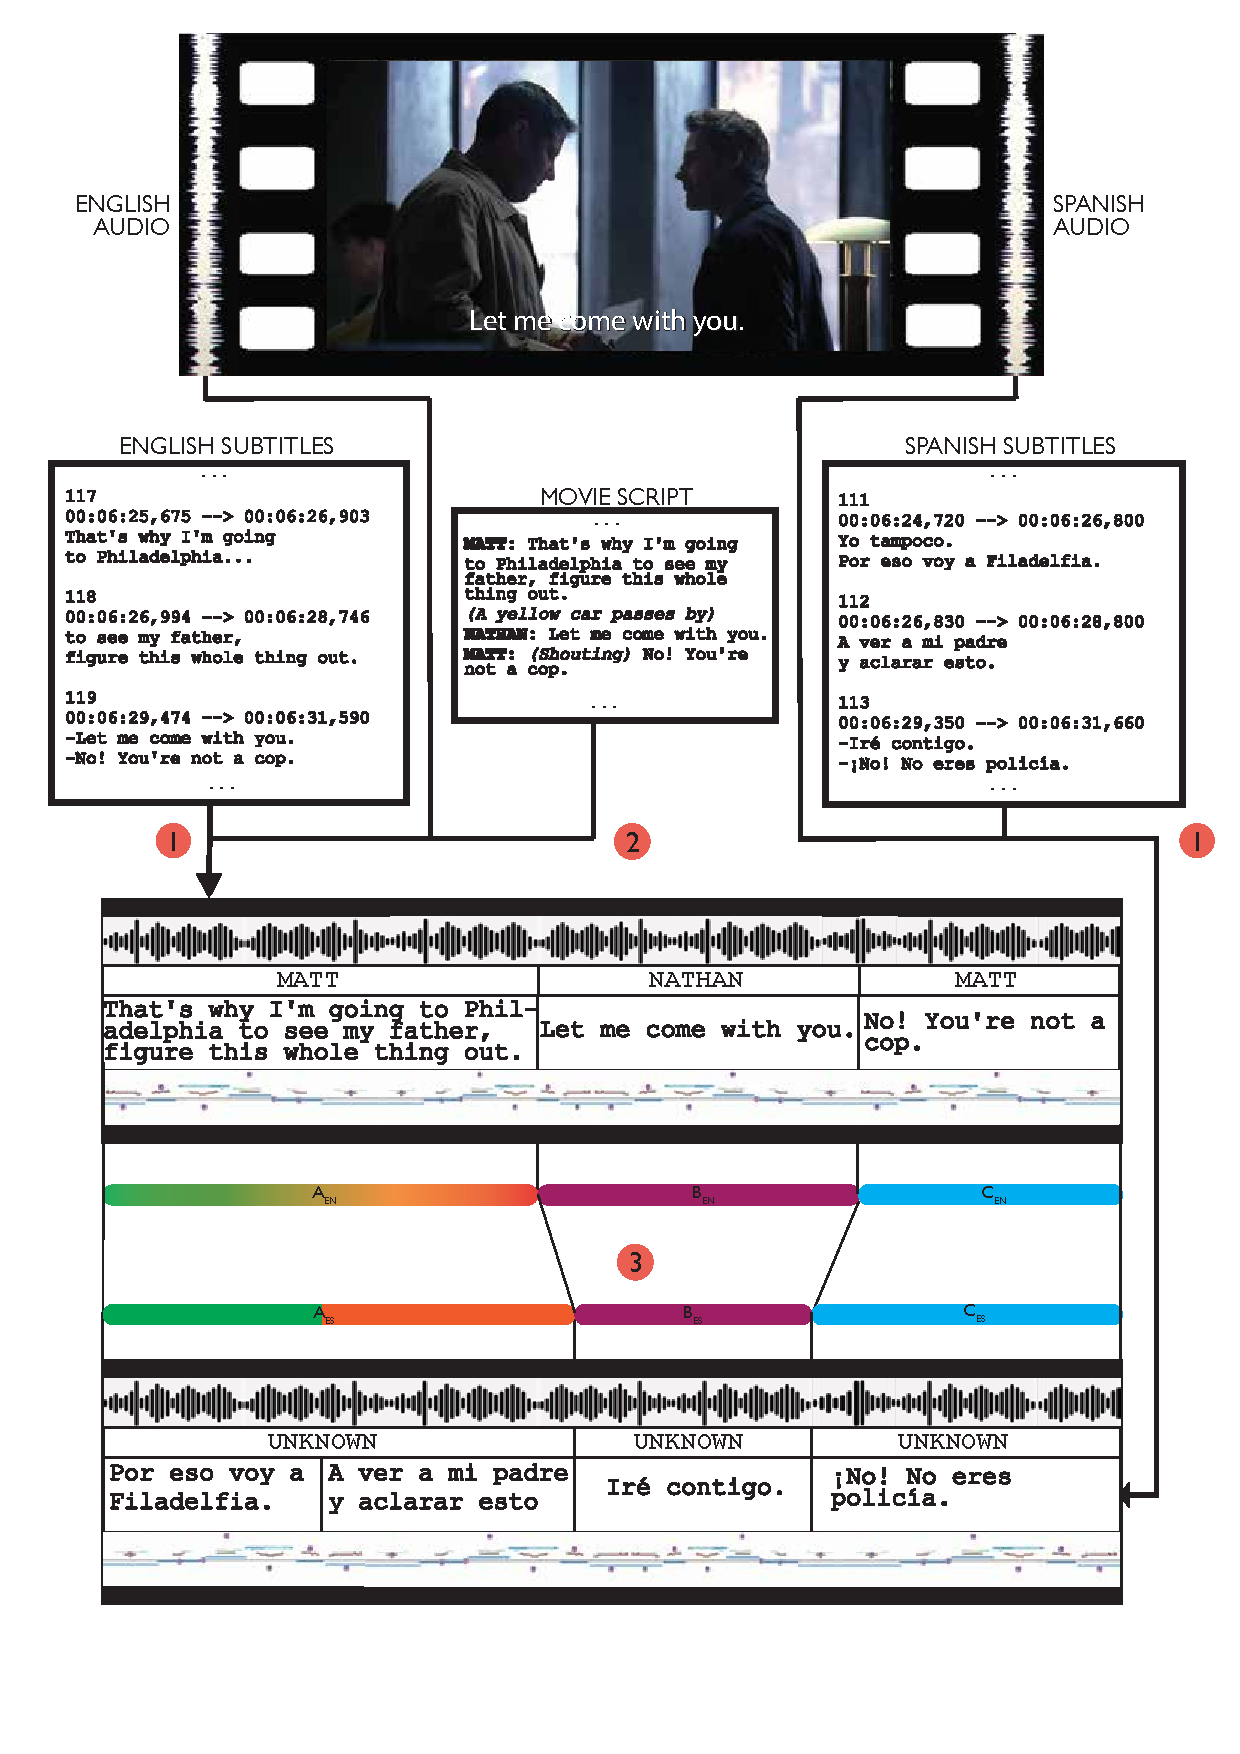
\includegraphics[width=\linewidth]{img/movie2parallelDB/movie2parallelDB-example_pipeline.pdf}
      \caption{Processes 1,2 and 3 of the methodology illustrated on a portion of a movie. }
      \label{corpusWorks:fig:example_pipeline}
    \end{figure}
    \clearpage
}

% \begin{figure}
% \centering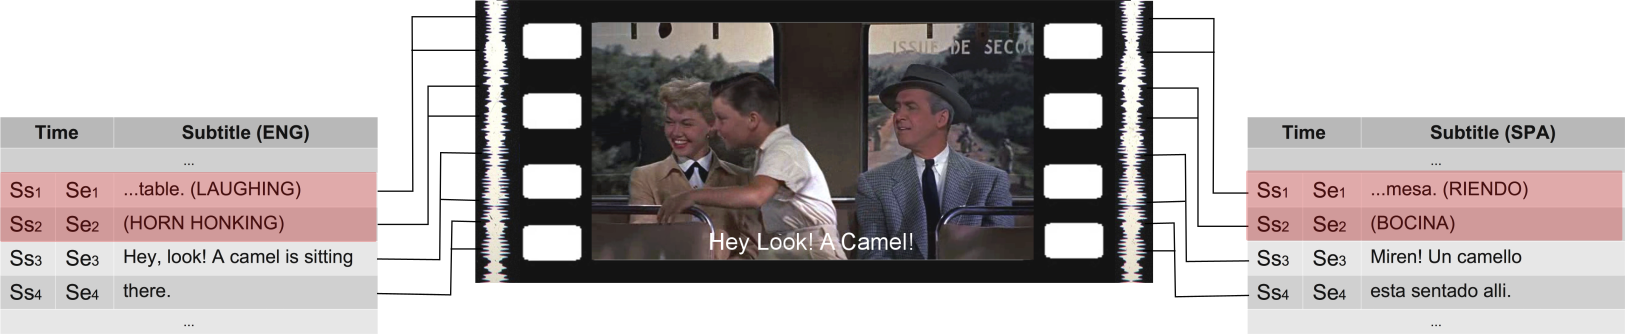
\includegraphics[width=\linewidth]{img/movie-as-parallelDB.png}
% \caption{Aligning parallel speech and subtitle segments in a dubbed movie. (Still from 1956 movie \textit{The Man Who Knew Too Much})}
% \label{corpusWorks:figure:parallel_segments}
% \end{figure}

% Explanation of the overall methodology. 
The methodology for obtaining a parallel corpus from a dubbed media consists of three stages: (1) a monolingual step, where audio+text pairs are extracted from the movie in both languages using transcripts and cues in subtitles, (2) paralinguistic feature annotation (speaker information and prosody) and (3) alignment of monolingual material to extract the bilingual segments. See Figure \ref{corpusWorks:fig:overall-scheme} for an overview of the system pipeline. Figure \ref{corpusWorks:fig:example_pipeline} further illustrates the whole process on an example portion of a movie. Following subsections explain in detail each process. 

\begin{figure}[t]
  \centering
  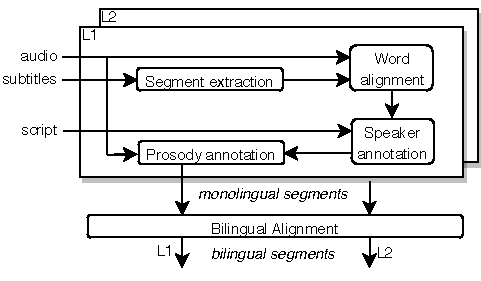
\includegraphics[width=0.6\linewidth]{img/movie2parallelDB/movie2parallelDB-pipeline.pdf}
  \caption{Overall corpus extraction pipeline. Audio excerpts are first processed in each language and then aligned to obtain bilingual segments.}
  \label{corpusWorks:fig:overall-scheme}
\end{figure}

\subsection*{Audio segment mining using subtitles}
Subtitles are the source for obtaining both (1) audio transcriptions, and (2) timing information related to utterances in a movie. These information are contained in a standard \textit{srt}\footnote{SubRip text file format \url{https://www.matroska.org/technical/specs/subtitles/srt.html}} subtitle file, entry by entry like the structure below:

\begin{lstlisting}
1
00:06:25,675 --> 00:06:26,903
That's why I'm going
to Philadelphia...
2
00:06:26,994 --> 00:06:28,746
to see my father,
figure this whole thing out.
3
00:06:29,474 --> 00:06:31,590
-Let me come with you.
-No! You're not a cop.
\end{lstlisting}

Each subtitle entry is represented by an index, time cues and the script being spoken at that time in the movie. The script portion can consist of multiple (\#2), complete \toni{TODO:next \2,3 $\to$ \#3? I mean, if sentence is "That's why ... thing out.", 2 does not seem complete}(\#2,3) or incomplete sentences (\#1) and from single (\#1,2) or multiple speakers (\#3). Using only these time cues does not suffice for extracting audio segments with complete sentences of a single speaker. To achieve this, word boundaries extracted with Montreal Forced Aligner is combined with punctuation mark positions to split and merge segments as needed. Two entries are merged if the first one does not end with a sentence-ending punctuation mark and the second one starts with a lowercase letter. Multi-speaker segments were split from the words following speech-dashes. This process is marked with the label "1" on Figure \ref{corpusWorks:fig:example_pipeline}.



The resulting segments from the subtitle excerpt from above would be:
\begin{enumerate}
    \item That's why I'm going to Philadelphia to see my father, figure this whole thing out.
    \item Let me come with you.
    \item No! You're not a cop.
\end{enumerate}

\subsection*{Speaker annotation through scripts}
Movie scripts, which contain dialogue and scene information, are valuable pieces of information for determining the segment speaker labels. Scripts follows approximately the same format: Actor/actress name is followed by the line they say. In between, there might be non-spoken information in brackets. An example excerpt from a movie script of TV series \textit{Heroes} is given below:

\begin{lstlisting}
MATT:   That's why I'm going to Philadelphia to see my father, 
        figure this whole thing out.
        (A yellow car passes by)
NATHAN: Let me come with you.
MATT:   (Shouting) No! You're not a cop.
\end{lstlisting}

Unlike subtitles, scripts do not have timing information. In order to map subtitle segments with the speaker information, an automatic procedure is followed. First, all non-spoken text included in brackets is removed. Then, speaker tags and corresponding lines are extracted with regular expressions depending on the format of the script. Next, segments coming from subtitles are mapped one by one to lines in the script. If 70\% of the words in a subtitle segment is included in a script turn, then the segment is labeled with the speaker of that turn. If it doesn't, up to five next script turns are checked as candidates. 

It should be noted that scripts are usually only available in the original language. However, since segments are aligned on a later step with their dubbed matches, they can share the speaker labels. In Figure \ref{corpusWorks:fig:example_pipeline}, speaker labels are extracted from the English script and matched with the subtitles. Spanish segments are left with an "UNKNOWN" label until they are aligned with their respective English counterparts. 

\subsection*{Word-level acoustic feature annotation}

Each word in the extracted segments is automatically annotated with the following acoustic features: mean fundamental frequency (f0), mean intensity, speech rate and silence intervals (pauses) before and after. The first two features are extracted with \textit{ProsodyTagger}. Pause information is calculated from word-boundary information and speech rate is calculated using:

\begin{equation}
  word\,speech\,rate = {\dfrac{\#syllables\,in\,word}{word\,duration}}
  \label{sprate}
\end{equation}

To represent speaker independent, perceptual acoustic variations in the segments, both f0 and intensity values are converted into logarithmic semitone scale relative to the speaker norm value. Thus, speaker mean values were represented by zero values in both cases. Semitone values are calculated with the corresponding formula:

\begin{equation}
  semitone(x, norm) = 12 * \log (\dfrac{x}{norm})
  \label{semitone}
\end{equation}

The prosodic annotations are shown under the extracted segments with Prosograph feature visualizations in Figure \ref{corpusWorks:fig:example_pipeline}.

\subsection*{Cross-lingual segment alignment based on subtitle cues}
\label{subsec:alignment}
The first three methodologies presented in this section dealt with extraction of segments in each language. Audio and subtitle pair of each language result in a number of speech segments. This subsection explains how these segments are aligned to create the bilingual segment pairs. 

As explained earlier, the dialogues in the original and dubbed language correspond to each other time-wise. So, in order to align segments extracted for each language, timing information of the segments can be exploited. However, as subtitles show slight differences, alignment cannot be performed one-to-one. Number of segments extracted from each language can differ. This means that the segment alignments can be one-to-one, one-to-many, many-to-one or many-to-many depending on the sentencing structure in the subtitles. 

In order to create an alignment algorithm based on time cues, a metric is defined that measures the correlation percentage between two sets of ordered segments S=$\langle s_1, ...,  s_N\rangle$ and E=$\langle e_1, ...,  e_N\rangle$:
\begin{equation}
    segments\,correlation = max(0,\dfrac{correlating}{span} \times 100)
\end{equation}
\begin{equation}
    correlating = min(e_N^s, s_N^e) - max(s_1^s, s_1^s)
\end{equation}
\begin{equation}
    span = max(e_N^e, s_N^e) - min(e_1^s, s_1^s)
\end{equation}

where $e_x^s$ and $e_x^e$ denote the starting and ending time of the $x^{th}$ segment in set E, $s_x^s$ and $s_x^e$ denote the starting and ending time of the $x^{th}$ segment in set S. 

The alignment procedure is as follows: two indexes $i_E$, $i_S$ are kept which slide through the segments of each language. First, segments corresponding to each index are checked if they correlate more than the $T_{Sure}$ threshold. If they do, they are assigned as a one-to-one matched pair. If not, the possibilities of one-to-many, many-to-one or many-to-many matches are considered. This is done through computing the correlations between combinations of the current and two following segments and selecting the most correlating segment set pair. While considering combinations of the segments it is made sure that two merged segments belong to the same speaker and are not more than 10 seconds far from each other. If the combined segment set pair with highest correlation has a correlation of more than $T_{Merged}$ threshold, then the combinations are merged into one segment and paired with each other. 

Although the $T_{Sure}$ threshold catches most of the one-to-one mapping segments, many of them still fall below this threshold even if they map. So, another decision step is added where if one-to-one mapping correlation scores higher than merged pairings and it scores above a $T_{OK}$ threshold, then it is preferred as a matched pair. 

Figure \ref{corpusWorks:fig:example_pipeline} illustrates two examples of segment matching. First two Spanish segments are merged to align with the first English segment. Following segments are aligned one-to-one as their durations correlate enough. 

\toni{TODO: Explain a little bit more the figure. For instance, add "the speakers are labelled in the source language and paired in the target language"}


\subsection*{Using the parallel corpus extraction framework}
This methodology is developed as a open source framework called \textit{movie2parallelDB} and is accessible online \footnote{\url{github.com/alpoktem/movie2parallelDB}}. The usage instructions are included in the online repository. 

The scripts are run with audio and their corresponding subtitles. Therefore, audio tracks needs to be extracted from the respective video prior to the process. Matching subtitles also needs to be acquired. 
One challenge that this method poses is that although it is easy to find subtitles in both original and dubbed languages of a movie, dubbing script might differ from subtitles. This is due to the difference in process between subtitling and dubbing. As it is mandatory to obtain exact transcription of the audio segments, subtitles need to be corrected prior to the process. 

\section{Compiling the \textit{Heroes Corpus}}
\label{corpusWorks:heroes}
The methodology presented in the previous section was put into practice by compiling a corpus from 2000's popular science fiction TV series \textit{Heroes}\footnote{Produced by Tailwind Productions, NBC Universal Television Studio (2006-2007) and Universal Media Studios (2007-2010)}. Originating from United States, Heroes ran in TV channels worldwide between the years 2006 and 2010. The whole series consists of 4 seasons and 77 episodes and is dubbed into many languages including Spanish, Portuguese, French and Catalan. Each episode runs for a length of 42 minutes in average. 

\subsection*{Raw data acquisition}
The DVD's of the series were obtained from the Pompeu Fabra University Library. Episodes were extracted using the \textit{Handbrake} software and were saved as \textit{Matroska format (mkv)} files. Mkv files can hold multiple channels of audios and subtitles embedded in it like DVDs. In order to run \textit{movie2parallelDB} scripts, audio and subtitle pairs for both languages needed to be extracted. Audio is extracted using the \textit{mkvextract} command line tool\footnote{\url{https://mkvtoolnix.download/}}. As subtitles were embedded as bitmap images in the DVD, an optical character recognition (OCR) software\footnote{Through a functionality provided by Subler: \url{https://subler.org/}} was used to convert them to \textit{srt} format subtitles. As OCR is an error-prone process, the resulting srt files needed to be spell checked. 

In total, 21 episodes were processed to obtain 25 hours English and Spanish audio with their corresponding subtitles. The episode scripts were obtained from a fan web page\footnote{\url{https://heroes-transcripts.blogspot.com/}}. 

\subsection*{Manual subtitle correction work}
The Spanish subtitles needed slight correction in order to match the Spanish audio. The reason for this mismatch was explained in the previous subsection. As dubbing and subtitling are two distinct processes, there often are differences. It was observed that the Spanish subtitle transcripts were matching the Spanish audio in approximately 80\% of the cases. As exact correspondence between audio and transcription was aimed, a correction process was carried out. Both subtitle transcripts and time-stamps had to be corrected to match exactly what is being spoken on the dubbing audio and when. This process was done using a subtitle editing program \textit{Aegisub}\footnote{\url{http://www.aegisub.org/}}. 

An advantage the manual correction process gives is the opportunity to filter out unwanted audio portions that would otherwise end up in the corpus. This process is necessary especially in the case the source material is noisy. During the correction process, subtitle segments that contained noise and music, overlapping or unintelligible speech and speech in other languages (e.g.~Japanese) were removed. The spell checking and timestamps and script correction of 21 episodes was done by two annotators and took 60 hours in total. 

For each episode to be processed, the annotators were provided with the episode video, English and Spanish subtitles extracted with the OCR software. The correction procedures for each episode are as follows:
\begin{enumerate}
    \item Automated correction of OCR errors in English subtitles.
    \item Manual correction of English subtitles with a spell checker.
    \item Automated correction of OCR errors in Spanish subtitles.
    \item Manual correction of Spanish subtitles with a spell checker.
    \item Proofing and correction of the Spanish subtitles.
\end{enumerate}

The automated correction process involved a basic substitution procedure for the character errors that the OCR software did consistently. For example the letter `ñ' would be mistaken almost always as `fi' or `I's would be mistaken as lowercase `L's. For further non-standard errors, the spell checker provided in \textit{Aegisub} software was employed. Each spelling mistake in the subtitles were replaced with its corrected version.

\begin{table}[]
\begin{tabular}{|>{\arraybackslash} m{0.48\linewidth} | >{\arraybackslash} m{0.48\linewidth} |}
\hline
\textbf{Subtitle Entry} & \textbf{Audio Transcript}           \\
\hline
\begin{tabular}[c]{@{}l@{}}-Te presento a tu compañero.\\ -¿Me vas a cambiar?\end{tabular} & \begin{tabular}[c]{@{}l@{}}-Te presento a tu compañero.\\ -¿Me cambiar\'as?\end{tabular} \\
\hline
Me han tenido dos años, pensar\'an que los abandoné. & Me han tenido encerrado dos años, pensaran que los abandoné.    \\
\hline
Discutimos,...   & Empezamos a discutir...  \\
\hline
\begin{tabular}[c]{@{}l@{}}-Nunca quise...\\ -Cierra la boca! Escucha.\end{tabular} & \begin{tabular}[c]{@{}l@{}}-Yo nunca quise...\\ -Cierra la boca! Escucha.\end{tabular} \\
\hline
Hablaremos cuando vuelva, ¿vale? & Hablaremos mas cuando vuelva, ¿vale? \\
\hline
\end{tabular}
\caption{\label{corpusWorks:table:heroes_proofing}A selection of non-matching subtitle entries and dubbing scripts in Heroes series episodes.}
\end{table}

Last step involves checking of the transcripts and timings of each entry in the Spanish subtitles. Entries that do not correspond to the speech in the dubbed audio are corrected. Also, start and end time of the subtitle entries are adjusted so that it fits perfectly to the spoken segment. See Table \ref{corpusWorks:table:heroes_proofing} for a selection of entries that show difference in transcript between subtitle entries and dubbing transcript. Depending on the episode, about 10\% to 20\% of the subtitle transcript needed to be corrected. 

\subsection*{Heroes corpus in numbers}

Statistics of the first preparation sprint of \textit{The Heroes Corpus} are presented in this section. 21 episodes from season 2 and season 3 were processed. Total audio durations of 7000 parallel segments is about 9.5 hours (see Table \ref{tab:duration}). Counts of several linguistic units in the final parallel corpus are presented in Table \ref{tab:counts}. A summary of how much of the content in one episode ended up in the dataset in average is presented in Table \ref{tab:episode}.  

\begin{table}[ht]
\centering
\begin{tabular}{|>{\centering\arraybackslash} m{0.48\linewidth} >{\centering\arraybackslash} m{0.17\linewidth} >{\centering\arraybackslash} m{0.17\linewidth} |}
\hline
 & \textbf{English} & \textbf{Spanish}\\ \hline
\textit{Total duration} &  4:45:36 & 4:43:20 \\
\textit{Avg. duration/segment} & 0:00:02.44 & 0:00:02.42 \\\hline 
\end{tabular}
\caption{\label{tab:duration}Corpus duration information.}
\vspace{-7mm}
\end{table}

\begin{table}[ht]
\centering
\begin{tabular}{|>{\centering\arraybackslash} m{0.48\linewidth} >{\centering\arraybackslash} m{0.17\linewidth} >{\centering\arraybackslash} m{0.17\linewidth}|}
\hline
 & \textbf{English} & \textbf{Spanish} \\ \hline
\textit{\# words} &  56320 & 48593  \\
\textit{\# tokens} & 72565 & 63014 \\
\textit{\# sentences} & 9892 & 9397 \\ 
\textit{Avg. \# words/sentence} & 5.69 & 5.17 \\ 
\textit{Avg. \# words/segment} & 8.04 & 6.94 \\ 
\textit{Avg. \# sentences/segment} & 1.41  & 1.34 \\ \hline 
\end{tabular}

\vspace{5mm}
\begin{tabular}{lrr}
\toprule
 \textbf{Counts}             & \textbf{English} & \textbf{Spanish} \\ \midrule
{\# words}                  & $56\,320$ & $48\,593$  \\
{\# tokens}                 & $72\,565$ & $63\,014$ \\
{\# sentences}              & $9\,892$  & $9\,397$ \\ 
{Avg. \# words/sentence}    & $5.69$    & $5.17$ \\ 
{Avg. \# words/segment}     & $8.04$    & $6.94$ \\ 
{Avg. \# sentences/segment} & $1.41$    & $1.34$ \\ \bottomrule
\end{tabular}

%\toni{I use this format. If you like, use it, but I am perfectly ok with the other one}

\caption{\label{tab:counts}Word, token, sentence counts and average word count for parallel English and Spanish segments.\toni{TODO:explain somewhere roughly what are tokens}}
\vspace{-1mm}

\end{table}



\begin{table}[ht]
\centering
\begin{tabular}{|>{\centering\arraybackslash} m{0.50\linewidth} >{\centering\arraybackslash} m{0.15\linewidth} >{\centering\arraybackslash} m{0.15\linewidth}|}
\hline
 & \textbf{English} & \textbf{Spanish} \\ \hline
\textit{Avg. \# sentences (subtitles)} &  647 & 554  \\
\textit{Avg. \# sentences (extracted)} & 628 & 513 \\
\textit{Avg. \# segments} & 526 & 459 \\
\textit{Avg. \# parallel segments} & \multicolumn{2}{c|}{334}\\
\hline 
\end{tabular}
\caption{\label{tab:episode}Averages numbers for each episode. }
% \toni{I would have used absolute numbers (not by episode), as these are more easily compared with table 3.3 and 3.4}
\vspace{-6mm}
\end{table}

\subsection{Discussion}
The first version of the Heroes corpus shows that the proposed methodology for bilingual corpus building is successful in terms of the quality of the segments extracted. Our manual inspections show that the segments are correctly aligned and the transcriptions are correctly stored with the audio segments in general. 

The Spanish subtitle correction task was the only time-consuming part of the whole process. However, the task showed its usefulness for obtaining clean parallel segments. Subtitle segments that were removed during the correction process ensured the elimination of unwanted audio portions. 

Table \ref{tab:episode} shows the amount of information loss at various stages. The first one being the word-alignment process where in average 5\% of the sentences are lost due to the failure of the word aligner in segmenting words. Many of the segments that are lost this way were either noisy or erroneous. The biggest loss happens at the stage of alignment where in average 30\% of the segments in each language are left unaligned. This percentage is directly affected by the alignment parameters explained in Section \ref{corpusWorks:movie2parallelDB}. For example, selecting a lower $T_{Sure}$ leads to detecting more aligned segments but also to more mismatches. A similar logic applies to $T_{OK}$. Also, choosing a lower $T_{Merged}$ leads to more coverage of the sentences but \toni{again more ... rewrite this sentence} more as combinations with others, leading to fewer and longer segments. After experimenting with a handful of parameter combinations, this parameter combination proved to be the most optimal for this task: $T_{Sure} = 70 \%$, $T_{Merged} = 80 \%$ and $T_{OK} = 30 \%$.

\toni{TODO: In previous paragraph: first you use \emph{word aligner} and the \emph{stage of alignment} The second one, put adjective to the new alignment. E.g.: \emph{language-pair alignment ?}}

\toni{TODO: The sentence \emph{more as combination with others} sounds not very english to me, and repeat more. Maybe is enough
"Also, choosing a lower $T_{Merged}$ leads to more coverage of the sentences but leading to fewer and longer segments. "}

% \toni{In the paper copy, you striked out the next sentence:}

% \sout{The corpus is made accessible with \textit{Attribution-ShareAlike 4.0 International license}\footnote{creativecommons.org/licenses/by-sa/4.0/} through this link: \url{hdl.handle.net/10230/35572}. }

\section{\textit{Prosograph} for Aiding Study of Large Speech Corpora}
\label{corpusWorks:prosograph}
Prosody conveys several communication elements such as meaning, intention, and emotions, among others. Being able to clearly visualize the different elements involved in prosody --intonation, rhythm, and stress-- may be helpful for computational prosody research. Several speech analysis tools (e.g. Praat \citep{boersma01}), together with derived scripts and tools \citep{xu2013prosodypro,mertens2004prosogram,praatontheweb} partially cover these needs by helping to visualize quantifiable speech features like fundamental frequency ($F0$) and intensity contours, word stress marking, or prosodic labeling. These tools work well when showing detailed analyses on data and visualizing one single utterance at a time, but fail in visualizing generalized word-averaged speech features of many utterances, e.g., a discourse or a collection of speech samples, at once.


\textit{Prosograph} was born from the need to study prosody of long segments of speech to see the relation of prosodic features with punctuation in text. Inspiration was taken from music scores and piano rolls that help reading and visualizing music. Similar to a musical analysis tool, Prosograph helps visualize acoustic and prosodic structure in speech together with its transcript. Also through an interactive interface it makes it easy to listen to any portion of the displayed speech to accommodate auditory analysis \citep{prosograph}. 

\subsection{Implementation}

Prosograph is written in Python mode of Processing\footnote{\url{py.processing.org/}} because of its simplified access to graphical and interactive interface. In order to simulate music scores, the speech prosodic features are plotted in the vertical axis over a temporal horizontal axis. Words are put in order together with pauses and punctuation, and the prosodic features are drawn under each corresponding word. An overview of the tool can be seen in Figure \ref{corpus:figure:prosograph_dump}.

Two modes of Prosograph have been implemented: monolingual (standard) mode and bilingual mode. Bilingual mode makes it possible to view aligned parallel corpora. Aligned samples are displayed side by side to accommodate e.g. prosodic comparison. Figure \ref{corpus:figure:prosograph2_dump} illustrates an overview of Prosograph in bilingual mode. 

\begin{figure}
\centering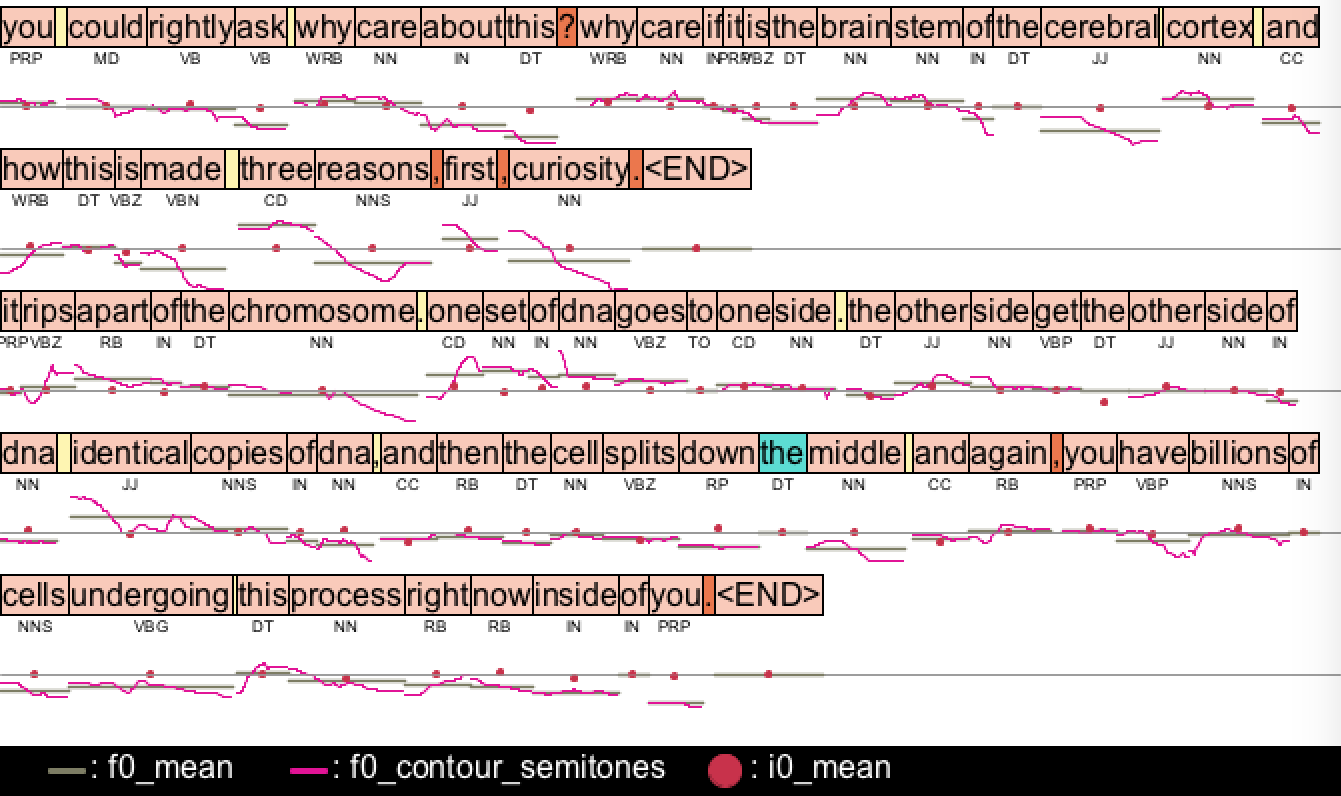
\includegraphics[width=\linewidth]{img/prosograph_dump_2.png}
\caption{An example of a visualization frame of segments from a conference talk with Prosograph.}
\label{corpus:figure:prosograph_dump}
\end{figure}

\begin{figure}
\centering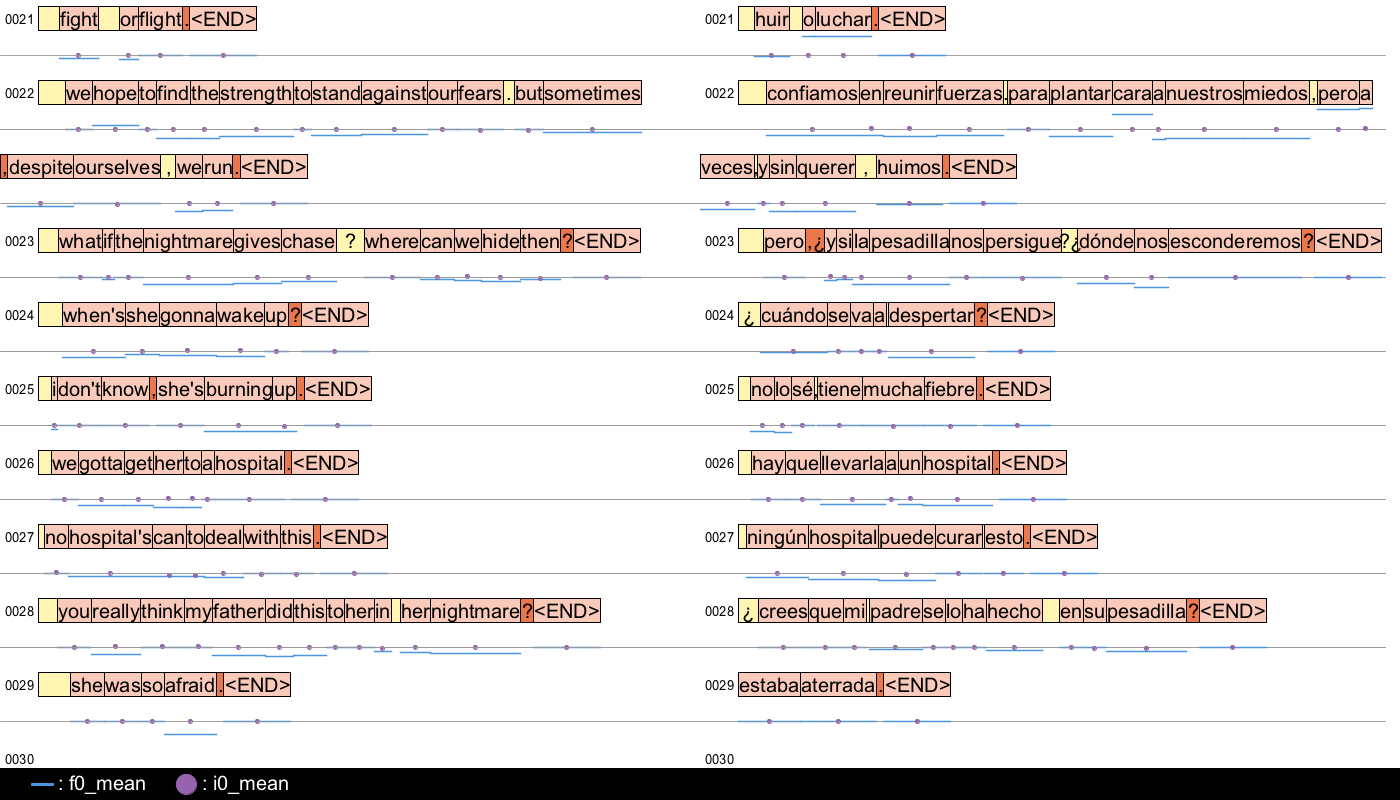
\includegraphics[width=\linewidth]{img/prosograph2_dump.png}
\caption{Visualizing parallel samples from an episode of Heroes Corpus with bilingual mode of Prosograph.}
\label{corpus:figure:prosograph2_dump}
\end{figure}

Prosograph reads prosodically annotated speech data from Proscript format files (see Section \ref{corpusWorks:toolkit}). Data path, and names and types of features in the files to be visualized has to be set in a configuration file before running the software. 

\subsubsection{Data types in Prosograph}
Prosodic features differ in the way they encode words or sentences. For instance, word stress is a feature that represents salience among a group of words, intonation and intensity are continuous encodings throughout successive voiced phonemes, accent is a peak that occurs at a certain point in a word, etc. Because of these variations each prosodic feature demands a special way for its storage and visualization. In order to visualize different types of prosodic encodings, following data sequence types that are encoded word-wise were compiled:

\toni{TODO: In previous par., check writting of: "that are encoded word-wise were compile"}


\toni{TODO: In the next list, you say "can be used", "could be used"; this suggest that the tool is customizabled by user, but no explained .. In fact it is explained later, but you should say something here, because I was expecting just the description of the tools}

\begin{itemize}
\item \textbf{pause-duration} holds the silence duration coming after the corresponding word. Paused intervals are visualized as an empty yellow box between words with a width proportional to the length of the pause (see Figure \ref{corpusWorks:fig:prosdatatypes}a).
\item \textbf{punctuation} holds the punctuation mark coming before or after the corresponding word. Punctuation marks are placed in the same axis with words. If a punctuation mark coincides with a pause, then it is placed inside the pause interval (see Figure \ref{corpusWorks:fig:prosdatatypes}b).
\item \textbf{binary-feature} holds a binary value determining if the corresponding word carries a certain feature (1) or not (0). This feature type can be used e.g. for word-stress. Bounding boxes of these words are drawn with a salient color (see Figure \ref{corpusWorks:fig:prosdatatypes}c).
\item \textbf{point-feature} holds a real numbered value that belongs to the corresponding word (e.g. standard f0 deviation, mean f0, median f0, etc.). It is placed at its value below the middle of the word's bounding box (see Figure \ref{corpusWorks:fig:prosdatatypes}d).
\item \textbf{line-feature} holds a real numbered value as point-features. They are visualized as a line below and parallel to the word. This feature type could be useful e.g. for visualizing better the mean f0 movement across the utterance (see Figure \ref{corpusWorks:fig:prosdatatypes}e).
\item \textbf{contour-feature} holds sequences of same length corresponding to each word. Each value is treated as curve bins and drawn as a line below the word in same length intervals. It is to be used e.g. for visualizing f0 curves or intensity curves or quantiles (see Figure \ref{corpusWorks:fig:prosdatatypes}f).
\item \textbf{percentage-feature} holds sequences of varying lengths where each value in the sequence corresponds to a percentage of time with respect to the duration of the word. A mark is placed at the corresponding time position below the word's bounding box. This feature type can be used e.g. to mark the point where the accent occurs in a word, f0 or intensity peaks (see Figure \ref{corpusWorks:fig:prosdatatypes}g).
\item \textbf{label-feature} holds a string label for their respective words. The label is written just below the respective word's bounding box. This feature type can be used to visualize prosodic labels such as ToBI or part of speech (see Figure \ref{corpusWorks:fig:prosdatatypes}h). 
\end{itemize}

\begin{figure}
\begin{tabular}{cc}
  
\includegraphics[height=4.5mm]{img/prosograph_datatypes/pause.png} &   
\includegraphics[height=4.5mm]{img/prosograph_datatypes/punctuation.png} \\
(a) pause-duration & (b) punctuation\\[6pt]
 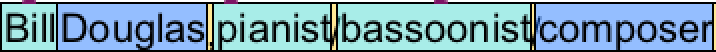
\includegraphics[height=4.5mm]{img/prosograph_datatypes/binary.png} &   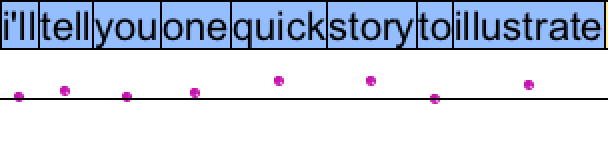
\includegraphics[height=11mm]{img/prosograph_datatypes/point.png} \\
(c) binary-feature & (d) point-feature\\[6pt]
 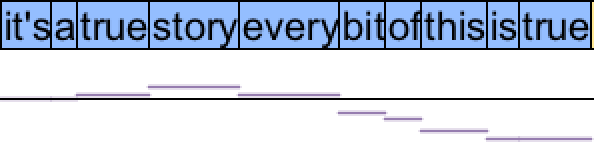
\includegraphics[height=11mm]{img/prosograph_datatypes/line.png} &   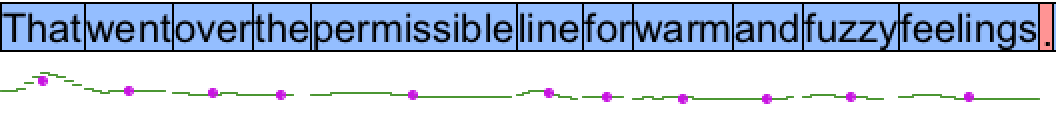
\includegraphics[height=8mm]{img/prosograph_datatypes/curve.png} \\
(e) line-feature & (f) contour-feature\\[6pt]
 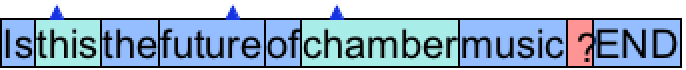
\includegraphics[height=6mm]{img/prosograph_datatypes/percentage.png} &   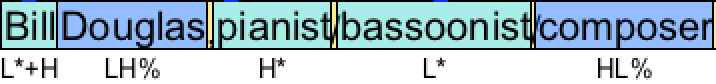
\includegraphics[height=7mm]{img/prosograph_datatypes/label.png} \\
(g) percentage-feature & (h) label-feature \\[6pt]
\end{tabular}

\caption{Word-aligned feature data types in Prosograph.}
\label{corpusWorks:fig:prosdatatypes}
\end{figure}

\subsection{Access and Usage}
Prosograph is made publicly available as an open-source software in the online repository \url{github.com/alpoktem/Prosograph} under the GNU General Public License\footnote{\url{http://www.gnu.org/licenses/}}. 

Once it is installed and the configurations are set, utterances in the dataset are shown in batches and user can navigate over the batches using keyboard shortcuts N(next) and B(previous). The current batch frame can be saved as an image by pressing S. 

%\toni{Just a comment: what a curious design that the colors are random at run-time!}

Colors of different prosodic features are set randomly at run-time. A legend showing which color belongs to which feature is shown at the bottom of the screen. If not easily distinguishable, the colors can be changed (again randomly) by pressing C on keyboard. 

To listen to a particular sample, beginning and end word of the utterance need to be selected. When P key is pressed, the utterance is played between the selected word interval. This is made possible if an audio file accompanies the Proscript file in the same directory with the same name. 

\subsection{Conclusion}
I have presented Prosograph, which can be used for the analysis of prosodic features and patterns in a speech corpus. It has been designed to be robust for handling different types of prosodic data annotated on word level. By simplifying the process of observation and comparison of prosody, this application can be used in many areas of research such as language learning and acquisition, comparative studies in different languages, tone languages, audiovisual prosody, etc.

Prosograph was first implemented to aid feature selection process in the punctuation restoration methodology that this dissertation presents in Chapter \ref{chapter:punkProse}. After its development, it was used to demonstrate the results of this system and to reason how a neural punctuation restoration system behaves with respect to various prosodic features. Through the development of the bilingual mode, it proved its use in studying prosodic transformations in the dubbed translations in the Heroes corpus and helped inspire the prosodically enhanced translation system that is to be presented in Chapter \ref{chapter:transProse}. Also, with its easy integration with Proscript library, it simplifies creation of visualizations of speech samples for linguistic study. Visualizations of speech samples in this dissertation are made with Prosograph. 

It should be noted that Prosograph is not a program that obligates its usage ``as-it-is''. It is a framework, written in a highly visual and experimental programming language to be customized to the needs of its user. For instance, a linguist wanting to observe certain characteristics in a recorded corpus can set it up to her like and display segments together with speaker information. The bilingual mode can be further extended to display utterances of two speakers together with a reference utterance and facilitate comparison. Another use-case could be real-time prosodic display and assessment for accent and intonation training. I hope the framework inspires researchers from different fields to study prosody and speech corpora in a visual and customizable way. 
\newpage\leavevmode\thispagestyle{empty}\newpage
% ---------------------------------------------------------------------

% CHAPTER 4: Punctuation works
% ---------------------------------------------------------------------
%**************** punkProse **************

\chapter{Punctuation Restoration Using Prosodic Cues}
\label{chapter:punkProse}

This chapter deals with the theme of punctuation restoration in speech transcripts focusing on its relation with prosody. My first aim is to convince the reader of the crucial role of prosody when determining placement of punctuation marks in raw speech transcripts (Section \ref{punkProse:motivation}). Next, the claims are further elaborated with some quantitative analyses on punctuation usage and prosody-punctuation relation in a corpus of conference talks (Section \ref{punkProse:analysis}). Then, I will present a deep learning based framework \citep{punkProse_slsp} for carrying out experiments on testing effects of various morphosyntactic and prosodic features on the task of punctuation restoration (Section \ref{punkProse:methodology}). Experiments explained in Section \ref{punkProse:experiments} focus on testing which feature set works best for the problem (\ref{punkProse:experiments:q1}), quantifying the influence of prosodic feature usage into dependency parsing quality (\ref{punkProse:experiments:q2}) and finally evaluating the system incorporated on a real speech recognition application (\ref{punkProse:experiments:q3}). Final remarks and conclusions are given in Section \ref{punkProse:discussion}. 

\section{Motivation and Background}
\label{punkProse:motivation}
The introduction of punctuation marks into the output of automatic speech recognition (ASR) is an important issue in applications such as automatic transcription/subtitling, speech-to-speech translation, language analysis, etc. Punctuation is essential for grammaticality, understandability, and --in the case of a number of different tasks--, subsequent processing. Thus, correct sentence segmentation and punctuation of recognized speech improves the quality of machine translation \citep{matusov2006automatic,peitz2011modeling, Cho2017NMTbasedSA, lu2010better}, and missing periods and commas in machine generated text results in sub-optimal information extraction from speech \citep{favre2008punctuating, hillard2006impact}. On a more end-user perspective, \cite{Tundik2018} show that punctuated captions are preferred by viewers of television shows in both manually and automatically generated transcriptions. Also, most of the data-driven parsing models require segmentation of recognized text into sentence like units and use punctuation as features \citep{Jones:1994:ERP:991886.991960, Spitkovsky_punctuation, MaPunc}. 

%linguistic sketch. 
%why is it needed?
Punctuation marks support understandability and readability in written language. Sentences generally form an enclosed unit with subject, object and verb and are marked by sentence-ending punctuation marks such as period, question mark and exclamation mark according to their modality (statement, interrogative etc.) Intra-sentence punctuation marks such as comma are required by certain syntactic phenomena like enumeration, clause separation, dislocation etc. In some languages (such as, e.g.~English), punctuation is also essential for the realization of the information structure \citep{Moore2016}. 

%what influences punctuation? syntax & prosody
In spoken language, punctuation of the transcribed speech is influenced by two intertwined phenomena: (1) syntax and (2) prosody. Syntax determines the distribution of punctuation marks in accordance with the orthography of a language. Prosody realization in speech (such as, e.g., word grouping, pausing, emphasis, rising-falling intonation, etc.) tends also to signal the position and type of the punctuation marks. As a matter of fact, it has been debated in history whether prosody is influenced by punctuation or vice versa \citep{wallace}. Early works on English grammar regard the use of punctuation as a mere symbology of how the language sounds. According to \cite{lowth} \textit{point marks} (period, colon, semicolon and comma) indicate breaks with different lengths, question mark and exclamation marks indicate ``an elevation of the voice'' and parentheses indicating a ``moderate depression of the voice''. Modern linguistic definitions, on the other hand, state that punctuation is directly dictated by grammatical rules with prosody influencing it from time to time \citep{algeo}. Regardless of a formal standpoint, it can be seen that prosody is related many times with punctuation. For instance, a pause after consecutive words might signal an enumeration, which requires comma, and rising intonation at the end of a sentence is a likely indicator of a question. Sentence and discourse boundaries are often marked with pauses and a reset in pitch. 

%Both prosody and syntax should be looked at when determining punctuation
During the manual transcription of an audio recording, both modalities, syntax and prosody, are used in determining the phrasing structure and punctuation. Example below illustrates the effect of prosody on punctuation, where the raw text could be punctuated in two different ways, eventually leading to two different meanings and syntactic structures. 

\begin{description}
\item [Raw] {\it and with all sincerity I can say I am glad I lived those two years of my life that way} 
\item [(1a)] {\it And with all sincerity, I can say, I am glad I lived those two years of my life that way.}
\item [(1b)] {\it And with all sincerity, I can say I am glad, I lived those two years of my life that way.}
\end{description}

\noindent Although it is ambiguous where to place the commas in this example just by looking at the transcription, by listening to the voice sample\footnote{Accessible from \url{github.com/alpoktem/punkProse/tree/master/audio-samples}}, there is only one possible punctuation: (1a), where {\it I lived those two years of my life that way} is a subordinated clause of {\it I am glad}. 

%buildup recent work
Many state-of-the-art approaches to automatic punctuation restoration are driven by textual criteria only \citep{Cho2017NMTbasedSA, lu2010better, ueffing2013improved, Gravano,  jakubicek2010punctuation, Che2016PunctuationPF}. However, it is proved that combination of prosodic and acoustic features with a textual model improves accuracy in ASR output \citep{baron2002automatic, khomitsevich2015combining, tilk2015lstm, tilk2016bidirectional}. Some approaches that use textual and prosodic models (or a combination of them) consider punctuation placement with narrow-range features such as n-grams \citep{liu2006study, khomitsevich2015combining, Psutka04automaticpunctuation}. Recent data-driven approaches that use recurrent neural networks (RNN)\footnote{Explained in Section \ref{sota:dnns}} proved to be competitive for the task due to RNN's ability to capture long and short term syntactic dependencies. These models, moreover, get use of word vectors which proves to capture well both syntactic and semantic structure of the language \citep{Treviso, Che2016PunctuationPF}. However, such neural models that account for prosodic features (e.g.~\cite{tilk2015lstm, tilk2016bidirectional}) rely merely on pause duration between words, while other prosodic features such as pitch and intensity information are ignored. Another shortcoming of these approaches is that the models are trained either only on written data \citep{ballesterosneural, Che2016PunctuationPF} or on a combination of written and spoken data (with, again, a dominance of written material) \citep{tilk2016bidirectional}. This makes the trained models biased towards written data. 

%So what... later-add
My motivation extends from the necessity seen in inclusion of prosody in a more complete way into the problem of punctuation restoration on raw speech transcripts. In applications where automatic speech recognition is employed, it is possible to integrate a prosodic feature extraction framework which would contribute to the accuracy of the punctuation placement. Also, there is no earlier study mentioning the individual and combined effect of various prosodic features (e.g.~intonation, intensity, speech rate) to the generation of various punctuation marks in a neural-network based setting. For these reasons, this chapter gives focus to the development of a framework that enables testing of various prosodic features in the problem of punctuation restoration. Furthermore, the applicability of the introduced model is put into test on two distinct settings. Firstly, the effect of prosodic punctuation restoration is studied on quality of dependency parsing which is a method often used in natural language processing (NLP) applications. Secondly, the methodology is put into test with a real ASR system. 

\section{Analyzing Punctuation in Conference Talk Transcripts}
\label{punkProse:analysis}
In this section, I will study the \textit{TED Talks Corpus} presented in Section \ref{corpusWorks:ted} in terms of punctuation usage and correlation of punctuation marks with pausing in speech. This kind of a quantitative analysis is performed both for helping design an automated methodology to solve the problem of punctuation restoration and also to help interpret its results. 

The speech style involved in conferences is usually defined as semi-spontaneous. This is for the fact that it is delivered without being read from a source text, however, with prior rehearsal possibly utilizing a written form of the talk. Although it restricts to a certain spoken language stype, it still gives a good estimation for extracting knowledge on punctuation placement for spoken language transcription. 

Both punctuation and the transcriptions analyzed are manually annotated by volunteers who watch and transcribe the talks. Punctuation marks and paragraph breaks are placed while listening to the talks at the same time of transcribing them meaning that they are related with the prosodic structure of the talk. See Figure \ref{punkProse:figure:ted_transcripts} for an example of the transcription structure available for the talks on TED's website. 

\begin{figure}[h]
\centering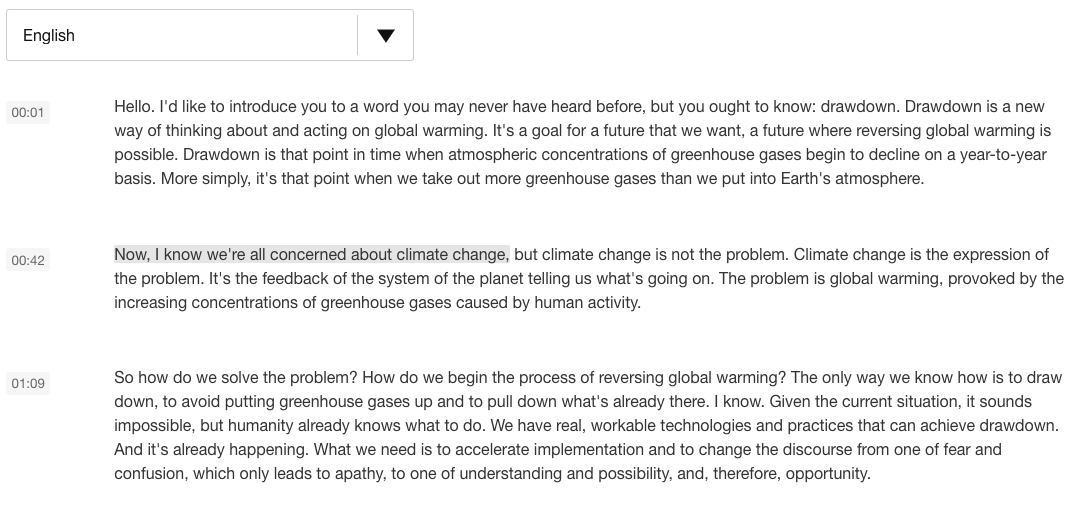
\includegraphics[width=0.9\linewidth]{img/ted_transcript_structure.png}
\caption{Transcription available in TED web page for the talk "100 Solutions to Climate Change" by Chad Frischmann.}
\label{punkProse:figure:ted_transcripts}
\end{figure}

The first analysis that I perform involves examination of the frequency of each punctuation mark in the dataset. As demonstrated in Figure \ref{punkProse:figure:punc-freq-pause-perc:a}, it is observed that the majority of the punctuation marks in the dataset consists of a comma and a period, corresponding to 94\% of all punctuation marks. As most of the talks go in the style of a monologue, questions are seldom made explaining the 3.7\% share of question marks. 

\begin{figure}[h]
\centering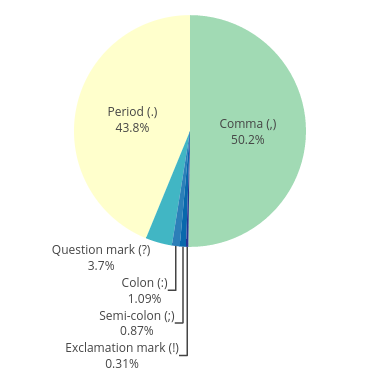
\includegraphics[width=0.6\linewidth]{img/1-ted-punc-freq.png}
\caption{Punctuation distribution in the transcripts of the TED Talks Corpus.}
\label{punkProse:figure:punc-freq-pause-perc:a}
\end{figure}

\begin{figure}[h]
\centering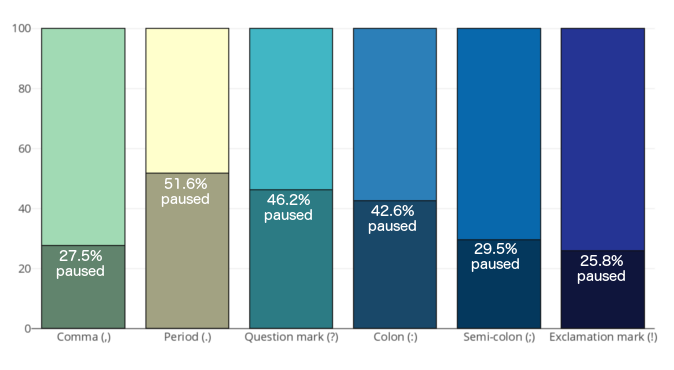
\includegraphics[width=0.6\linewidth]{img/2-pause-ratio.png}
\caption{Pausing percentage of each punctuation mark in TED Talks Corpus.}
\label{punkProse:figure:punc-freq-pause-perc:b}
\end{figure}

\begin{figure}[h]
\centering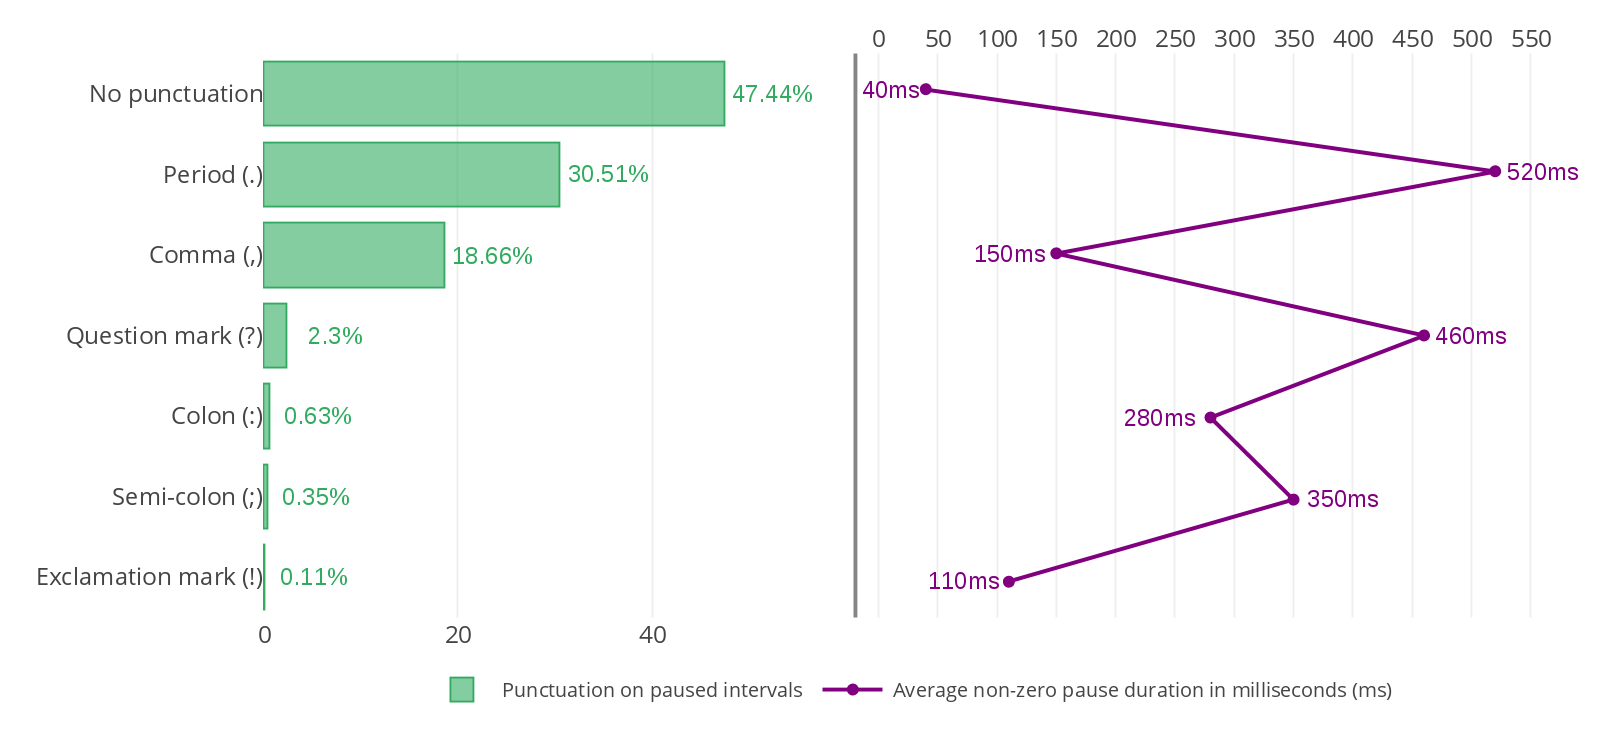
\includegraphics[width=\linewidth]{img/3-pause-events.png}
\caption{Distribution of punctuation presence in paused intervals (left) and corresponding average non-zero pause lengths of each punctuation mark (right).}
\label{punkProse:figure:punc-freq-pause-perc:c}
\end{figure}

Inter-word pauses in speech are known to be a pertinent prosodic feature in determining sentence and phrase boundaries, and punctuation marks \citep{Psutka04automaticpunctuation, Christensen01punctuationannotation}. The relation between inter-word pauses and punctuation is analyzed in two ways: First checked is the presence of a pause given that there is a particular punctuation mark, and second checked is the type of the punctuation mark given that there is a pause. Note that the pauses are defined as intervals in speech where no speech signal is detected. This information is obtained from the word alignments available in the corpus. 

Figure \ref{punkProse:figure:punc-freq-pause-perc:b} shows results of the first analysis. It is seen that sentence-ending punctuation marks are more likely to be accompanied by a pause. Most paused interval is where periods occur (51.6\%). This means that at most half of the sentence boundaries are actually marked by pause. Commas seem to be marked with a pause in only 27.5\% of the cases. 

Second analysis illustrated in Figure \ref{punkProse:figure:punc-freq-pause-perc:c} shows the pause-punctuation causality in the opposite direction. Paused intervals are analyzed in terms of the type of punctuation event occurring at that interval. Performing a binary analysis, it shows that more paused intervals (52.6\%) are punctuated than unpunctuated (47.4\%). However, the small difference indicates that it is only slightly more probable that a paused interval infers a punctuation than no punctuation. Moreover, it is seen that the distribution of the punctuation marks is reflected in the order of the frequency of the events. However, although there are more commas in the corpus than periods, the latter type shows to be much more likely to occur in a paused interval. 

With respect to durations of the pauses, right side of Figure \ref{punkProse:figure:punc-freq-pause-perc:c} shows the average of non-zero pause lengths that correspond to each punctuation event. Sentence-ending punctuation marks tend to correspond to longer breaks than commas. Excluding very rarely occurring punctuation marks (colon, semi-colon and exclamation mark), sentence boundary pauses are almost half a second in average. It is also seen that the 47.4\% of the pauses, the ones without any punctuation mark, are actually of very short duration in average (40 ms).

The quantitative analyses show that presence of pauses is not a discriminating feature by itself in determining the presence of a punctuation mark. However, length of the pause can be a good feature for both determining presence of a punctuation and also the type of the punctuation. Sentence-endings are more likely to be related with a break and if so, it indicates a longer break compared to commas. However, this distinction fails to show itself between different types of sentence-ending marks, period and question mark. This signals the necessity of other discriminative features, be it syntactic or prosodic, for the differentiation between them.

Another finding is that a data-driven model based on this dataset would be useful in classifying only a group of punctuation marks consisting of period, comma and question mark as the rest is not represented enough in this particular dataset. 

%A nice analysis could be pause length vs. punc presence. How do the first graph look if you put a threshold on pause length. 

\section{Methodology}
\label{punkProse:methodology}

%What motivates again?
As explained earlier in Sections \ref{sota:punk_on_asr} and \ref{sota:punk_prosody}, state-of-the-art on punctuation restoration shows advance with two main approaches (1) combination of prosodic and lexical features, and (2) employment of RNN-based architectures. A RNN-based architecture defines the problem as prediction of a punctuation class (including "no punctuation") at each position coming before or after a word input at each step, as in Figure \ref{punkProse:figure:he_who_knows}). The words are input to the network as vectors (using word embeddings) and are accompanied with prosodic features if there is a prosodic modelling involved.

\begin{figure}[h]
\centering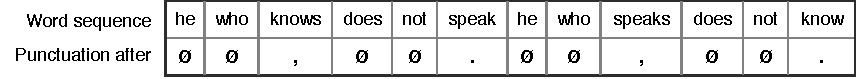
\includegraphics[width=\linewidth]{img/he_who_knows.pdf}
\caption{Modelling punctuation as a classification problem at each word interval. (Quote by \textit{Lao Tze})}
\label{punkProse:figure:he_who_knows}
\end{figure}

RNN-based work that combines lexical and prosodic features \citep{tilk2015lstm, tilk2016bidirectional} show incorporation of prosodic features into the punctuation modelling only through a limited dimension. Firstly, prosodic modelling is only limited within pauses used as sole prosodic feature. Secondly, prosodic modelling is done in a secondary training step which is the only step that involves introduction of spoken language. Model is biased on huge amounts of written data which shows differences in terms of both language and punctuation usage compared to spoken language. 

In this section I will address my motivation that prosody should be considered in a more complete way for the task of punctuation restoration. I will first define a set of features that could be used for modelling punctuation in spoken language within a neural network based setting. Secondly, I will explain a RNN-based architecture that is able to process this information and also allows testing of which prosodic features influence punctuation placement to what extent. 

\subsection{Features for Punctuation Modelling}
\label{punkProse:methodology:features}

Syntactic information proves to be one of the main features in modelling punctuation as in the works \cite{Che2016PunctuationPF, batista2012bilingual, ballesterosneural}. Syntactic influence to punctuation is defined by the grammatical rules of a language as well as sentence structure. Sentence boundary marking is the most common use of a punctuation mark. The type of the punctuation terminating a sentence is influenced by the modality of the sentence (statement, question, command etc.) Each of these modalities often influence which type of words are used in which order in the sentence. For example in English, a WH-question would include one of the WH-words (what, which, how etc.). Whereas a yes/no question can be discriminated by the order of the verb and subject (\textit{It is...} vs.~\textit{Is it...}). Usage of comma, which is a non-sentence-ending punctuation mark, is many times required by certain syntactic structures in a language again signaled by the lexical content. These include relative clauses or presence of initial temporal information as in examples below:

\begin{enumerate}
    \item \textit{Today, I will start jogging.}
    \item \textit{It is, however, extremely difficult to identify all the relevant variables.}
    \item \textit{Adam’s new van, which is less than a month old, makes a lot of noise.}
\end{enumerate}

A RNN-based network is able to model the language by processing sequences of words being represented as vectors. These vectors, which are also called \textit{word embeddings}, are able to represent words in their morphological forms capturing their semantics, syntactic behaviour and morphological structures \citep{ballesterosneural}. 

In the proposed methodology, as morphosyntactic features, word embeddings and part-of-speech (POS) tags are used. POS tagging of the words were available as a supporting syntactic feature for English language through the NLTK toolkit \citep{nltk}.

%Prosodic features
For modelling prosodic influence on punctuation generation, four main acoustic-prosodic features are employed: pauses, pitch, intensity and speech rate. Pause features indicates the duration of silence between previous word and the current word. As pitch and intensity features vary between speaker to speaker, a scaling method is used for these features to convert the measured values to relative scales. Fundamental frequency (F0) in Hertz and intensity in decibels are converted to scales relative to the speaker's norm using the expression:

\begin{equation}
  semitone(x, norm) = 12 * \log (\dfrac{x}{norm})
  \label{semitone_formula}
\end{equation}

\noindent This is done to ensure the prosodic features represent the variations with respect to the mean rather than absolute values that may differ across speakers.  

To align pitch and intensity features to the utterance, mean and range values are calculated at word level so that each word can be associated with the pitch and intensity level corresponding to it. Range values are calculated by subtracting the minimum pitch and intensity values respectively from the maximum pitch/intensity value in the contour corresponding to the word. If a word is unvoiced or a measurement fails, its mean and range values are set to 0 which corresponds to the speaker mean value in the normalized scale.

\cite{Farrus:SP:2016} states speech rate as a discriminating feature in determining paragraph boundaries. To test its effect on sentence boundaries, it is included as a feature as well. Speech rate is calculated at each word by dividing the number of syllables in that word with the word's duration. It is then normalized according to the speaker's mean value. 
A complete list of the features with their abbreviations is given in Table \ref{punkProse:table:features}.

\begin{table}[th]
  \centering
  \begin{tabular}{>{\arraybackslash} m{0.25\linewidth} | >{\arraybackslash} m{0.15\linewidth} }
    \toprule
    \textbf{Feature} & \textbf{ID} \\
    \midrule
    Word vector                 & word                  \\
    Part-of-speech tag			& pos				  \\
    Pause before                & pause                     \\
    Mean pitch                  & mean.f0                    \\
    Pitch range                 & range.f0          \\
    Mean intensity              & mean.i0               \\
    Intensity range             & range.i0                   \\
    Speech rate                 & speech.rate       \\
    \bottomrule
  \end{tabular}
  \caption{Morphosyntactic and prosodic features used in the punctuation restoration framework.}
  \label{punkProse:table:features}
\end{table}

\subsection{Model Architecture}
\label{punkProse:methodology:model}
%Explain the inspired baseline. 
The architecture of the model is inspired by the methodology presented in \cite{tilk2015lstm} and \cite{tilk2016bidirectional}. These works employ a 2-stage training approach, as depicted in Figure \ref{punkProse:figure:tilk_2stage}. Two recurrent neural networks (RNN) are chained where the first one processes the words and the second one adds pause duration between two consecutive words as an additional feature to the output of the first network. The two stage architecture is employed for the lack of audio data compared to text data. In \cite{tilk2016bidirectional}, the network is further enhanced to process words in two directions using a bidirectional recurrent network \citep{brnn} with attention. As RNN layers, \textit{gated recurrent units} (GRU) are used \citep{gru} which were explained earlier in Section \ref{sota:dnns}. 

\begin{figure}[h]
\centering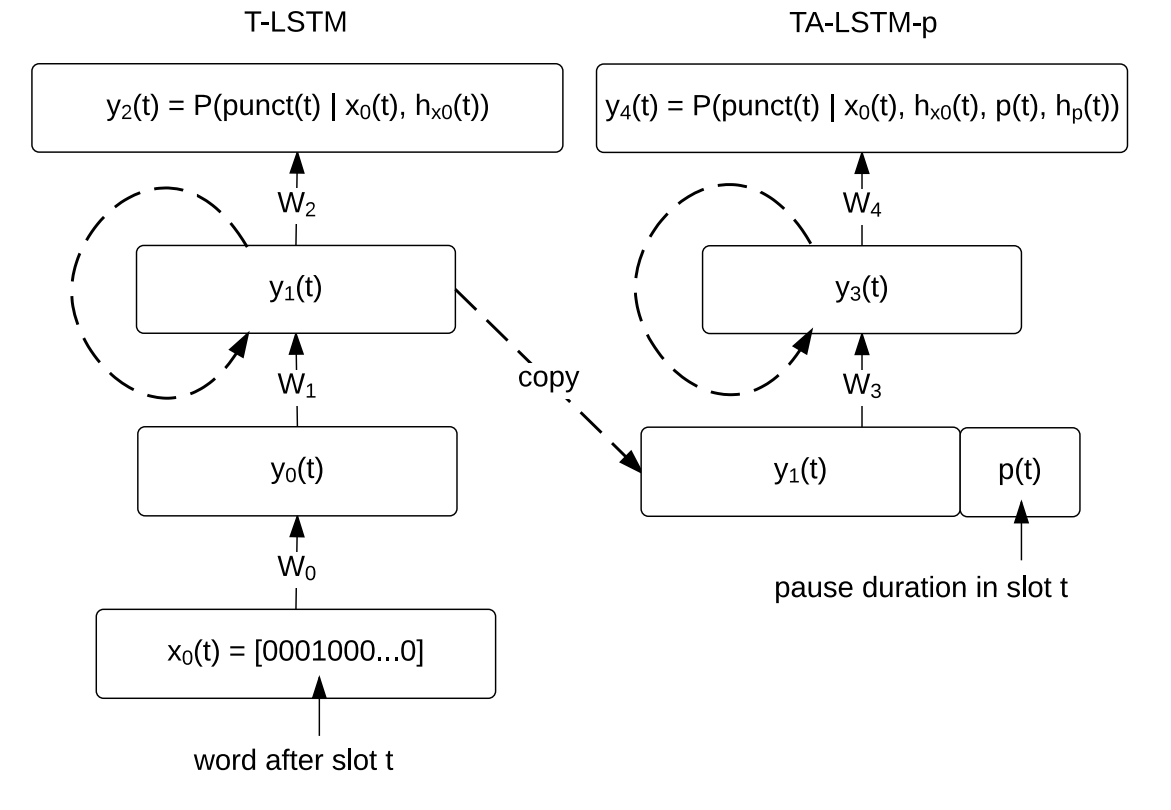
\includegraphics[width=0.65\linewidth]{img/tilk_2stage.png}
\caption{Two stage architecture of \cite{tilk2015lstm} (source of the diagram) which is later extended with bidirectional RNN layers in \cite{tilk2016bidirectional}. }
\label{punkProse:figure:tilk_2stage}
\end{figure}

%extension, expandable architecture
The modifications to Tilk and Alumäe's architecture are that (1) instead of passing prosodic feature values in a second stage, they are introduced to the model through separate parallel GRU layers that are tuned in one single stage, and (2) the proposed network is easily scalable so that it facilitates experimentation with different sets of features and configurations. The system can be configured to take any discrete features (e.g. word, part-of-speech (POS)) and prosodic features (e.g. f0 and intensity) to build a parallel layered network. Suprasegmental acoustic/prosodic features such as fundamental frequency, intensity and speech rate are aligned with words by taking the mean value corresponding to each word. 

\begin{figure}[h]
\centering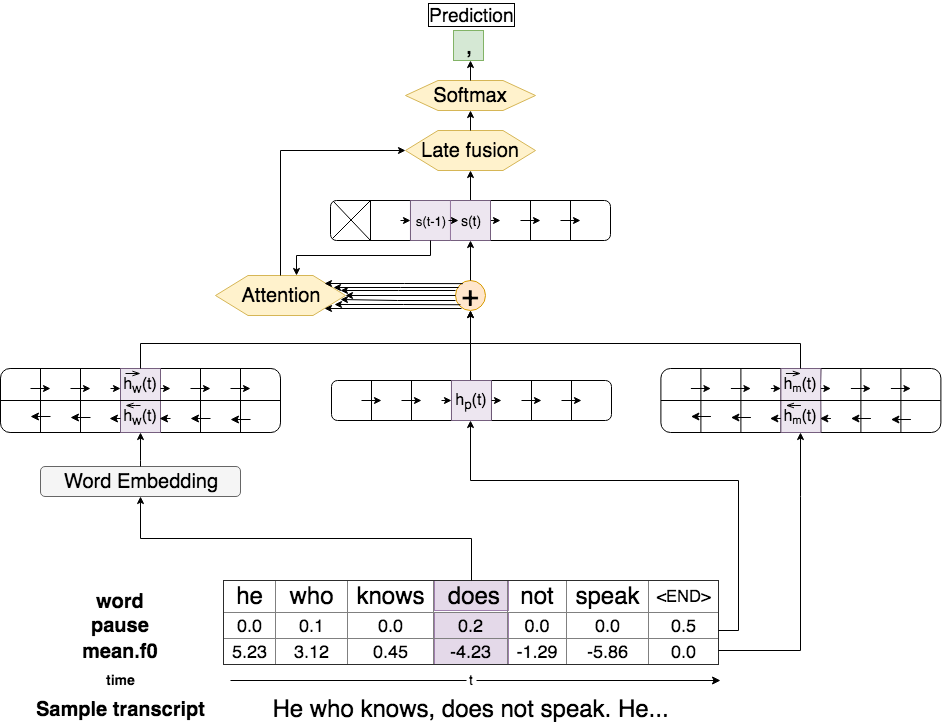
\includegraphics[width=\linewidth]{img/parallelRNNet_updated.png}
\caption{Our neural network architecture depicting processing of a speech data sample with pause and mean f0 features aligned at the word level.}
\label{architecture}
\end{figure}

I will now explain a possible model that could be generated by the proposed framework. For the sake of simplicity, the model will use as input: words ($w$) as the sole lexical feature and inter-word pause durations ($p$) and word-level pitch ($m$) as prosodic features. As for output, a punctuation class (period, question mark, comma or no punctuation) is given at training and predicted at inference. This architecture is illustrated in Figure~\ref{architecture}. It can be seen that, the model has 5 input GRU units: bidirectional layers for words, bidirectional layers for pitch values corresponding to words (denoted as \textit{mean.f0}), and a unidirectional layer for pauses coming before the words. Word GRU layers are preceded by an embedding layer ($W_{e}$). Inputs to the embedding layers are one-hot encoded vectors of sizes respective to the word vocabulary size. The hidden states of the GRU layers at time step $t$ are:

\begin{equation}
\overrightarrow{h_{w}}(t)~=~GRU(x(t)W_{e},~\overrightarrow{h_{w}}(t-1)) 
\end{equation}
\begin{equation}
\overleftarrow{h_{w}}(t)~=~GRU(x(t)W_{e},~\overleftarrow{h_{w}}(t+1)) \end{equation}
\begin{equation}
h_{p}(t)~=~GRU(p(t)W_{p},~h_{p}(t-1))
\end{equation}
\begin{equation}
\overrightarrow{h_{m}}(t)~=~GRU(m(t)W_{m},~h_{m}(t-1))
\end{equation}
\begin{equation}
\overleftarrow{h_{m}}(t)~=~GRU(m(t)W_{m},~h_{m}(t-1))
\end{equation}

\noindent where $x(t)$, $p(t)$ and $m(t)$ are the word index, pause duration and mean f0 value respectively at time step $t$. %and N is the sequence size.
The parallel GRU states are concatenated to form the context vector $h(t)$ before being passed over as input to another unidirectional GRU layer:

\begin{equation}
h(t)~=~\left[ \overrightarrow{h_{w}}(t), \overleftarrow{h_{w}}(t), h_{p}(t), \overrightarrow{h_{m}}(t), \overleftarrow{h_{m}}(t) \right] 
\end{equation}
\begin{equation}
s(t)~=~GRU(h(t),~s(t-1)) 
\end{equation}

The attention mechanism combines all input states into a weighted context vector $a(t)$, which is then late-fused with the state $s(t)$ of the output GRU layer:

\begin{equation}
a(t)~=~\sum_{i=1}^{N} h(t) \alpha_{t,i}
\end{equation}
\begin{equation}
f(t)~=~a(t)W_{fa}\bigodot\sigma(a(t)W_{fa}W_{ff}~+~s(t)W_{fs}~+~b_{f})~+~s(t) 
\end{equation}

\noindent where $\alpha_{t,i}$ is the weight that determines the amount of influence of each input state to the current output and N is sequence size. The late-fusion approach lets the context gradient carry on easily by preventing it to pass through many activation functions \citep{fusion}. Finally, the late-fused context $f(t)$ is passed through a \textit{Softmax} layer, which outputs a vector containing probabilities of the punctuation classes to be placed between the current and the previous word (starting from the second word in sequence): 

\begin{equation}
y(t)~=~Softmax(f(t)W_{y}~+~b_{y})
\end{equation}

Two key concepts introduced in \cite{tilk2016bidirectional} are: (a) bidirectionality and (b) attention mechanism. Bidirectional layers help to carry information from both past and future context with respect to the currently processed word. In the presented architecture, words as well as some prosodic features are processed bidirectionally. The attention mechanism is useful for the neural network to identify positions in a sequence where important information is concentrated \citep{bahdanau}. For words, it helps to focus on positions of words and word combinations that signal the introduction of a punctuation mark. For prosodic features, it either remembers a salient point in the sequence or detects a certain movement that could help determining a punctuation mark at a certain position. 

\section{Experiments}
\label{punkProse:experiments}

In this section, I will explain the implementation process of the proposed methodology regarding data preprocessing and selection of hyperparameters. Later, using the models obtained from various setups, I will explore the following questions through experimentation: 

\begin{enumerate}
    \item How do prosodic features in speech affect punctuation placement?
    \item What's the effect of punctuation presence to syntactic parsing?
    \item How do the obtained models perform within a speech recognition interface?
\end{enumerate}

\subsection{Data and Preprocessing}
%We use ted talks corpus blabla  sonra processing
Taking into account that the number of words per sentence in the TED Talks Corpus is 15--20 in average, the data is sampled into sequences of 50 words. Samples are extracted sequentially from talks. Each sample starts with a new sentence. Once no more complete sentences fit into the sample, the rest of the sample is padded with empty tokens. Sentences with more than 50 words are discarded. This was to ensure input to the system was complete so that the model always places a punctuation mark at the end of an utterance. Finally, a sample consisted of 2.6 sentences in average.

51,311 samples were extracted this way. 70\% percent (39,419 samples) of this data were allocated for training, 15\% for testing and 15\% for validation (8,446 samples each). The word vocabulary was created with the tokens that occur more than 6 times in the corpus and three extra tokens: \textit{out-of-vocabulary}, \textit{end-of-sequence} and \textit{empty}. This totaled up to 13,031 tokens. The output punctuation vocabulary in the experiments include 4 classes: period, question mark, comma and no punctuation. 

\subsection{Implementation and Hyperparameters}
\label{punkProse:methodology:implementation}
Theano \citep{theano} was used for implementing the models. In the experimental setup, the word embedding vector sizes for words were set to 100 which were initialized randomly at the beginning of the training. The hidden layer dimension of all GRU layers is also set to 100, except for pause durations and POS, where a smaller dimension of 2 and 10 respectively performed better in terms of validation scores. Besides words, mean pitch and intensity values are also processed in bidirectional RNN layers. 

The models were trained in batches of size 128. The weight matrices are updated using the \textit{AdaGrad} algorithm \citep{adagrad} with a learning rate of 0.05 for minimizing the negative log-likelihood of the predicted punctuation sequence. 

Two ways of inputting prosodic features into the model are tested. First, values are input as their absolute values in a continuous fashion, i.e.~pause durations in seconds, mean f0 values in semitones, intensity values in dB, and speech rate normalized within -1 and 1. Secondly, they are inputted as discrete values (in levels) and passed through an embedded layer similar to words and POS features. Leveling of the prosodic values was done by dividing each feature's normal distribution to quantiles of 100, so that more frequent ranges are represented more precisely. 

\subsection{How do prosodic features in speech affect punctuation placement?}
\label{punkProse:experiments:q1}
This section reports on the results obtained by training various models using different feature settings in terms of punctuation restoration accuracy. As the majority of the punctuation marks in the dataset consists of the punctuation marks in the reduced set (comma, period and question mark), experiments were performed only with this set.

The two-stage method by Tilk and Alumäe is used as a baseline by training over the data twice: first, only with text, and then together with the pause durations. Tilk et~al.'s models are based on BRNN with an attention mechanism, which provided the best results when compared to other models \citep{tilk2016bidirectional}.

In the proposed single stage approach, the use of only lexical information (words) provides the same scores as the use of only words in the two-stages approach, since only one step is involved in both approaches. In order to assess the contribution of new prosodic information to our model, more prosodic features were added one by one until no improvement is recorded. 

\subsubsection{Results}
The outcome of experiments in generating periods, commas and question marks with different settings of features are listed in Table \ref{scores} and illustrated in Figures \ref{overall-punk} and \ref{each-punk}. The results reported here use prosodic feature as continuous values in order to ensure comparability with the baseline. The best performing model was re-trained using discretized features and reported as well with the label \textit{discretized}. Additionally, a model with only prosodic features that ignores word information was tested (labeled as \textit{no words}). 

Compared to the two-stage models performance on the same dataset, first improvement is achieved through employing of the parallel processing architecture: An average improvement for all punctuation marks in terms of $F_1$ score of 0.4\% when the same features (word and pause durations) are used. The model opens the way for a further improvement of 2\% with the addition of pitch and POS feature into the model, and finally, with the introduction of discretized prosodic features, an overall $F_1$ score of 70.3\% is obtained.

By incrementally adding features on top of the word-based model, it is observed that usage of pause durations and part of speech (POS) improves period and question mark generation, and a combination of them results in an improvement in terms of $F_1$ score for all punctuation marks. The results also show that each punctuation mark has different sets of prosodic features that work the best for them. The best result for generation of commas in terms of $F_1$ score is observed with pause and pitch mean features (55.2\%). For period, mean intensity helps in terms of recall and a combination of it with pause and pitch mean results in best performing $F_1$ score of 82.0\%. For question mark, however, pitch and intensity features do not lead to an improvement, as the best result is achieved with the pause feature only (71.8\% $F_1$ score). 

Even without any textual features, silence, pitch and intensity features are able to determine sentence boundaries to a certain extent. A solely prosodic feature based model gives a precision of 71.3\% and an $F_1$ score of 55.7\% in detecting periods. When textual features are added to this set, it performs as the best model for generating periods. Although a sentence-ending punctuation mark, the question mark does not show the same behavior as it is much less represented in the dataset. 

The improved scores, which are achieved through discretization of continuous prosodic features, present new parameters of the neural network architecture that could be used to boost its accuracy. It proves that reducing the parameter space and representing leveled features in an embedded space can improve results in similar tasks. 

\begin{table}[tbp]
	\centering
	\scriptsize
	\begin{tabular}{p{4.4cm}>{\centering\arraybackslash}m{0.3cm}>{\centering\arraybackslash}m{0.32cm}>{\centering\arraybackslash}m{0.32cm}>{\centering\arraybackslash}m{0.32cm}>{\centering\arraybackslash}m{0.32cm}>{\centering\arraybackslash}m{0.32cm}>{\centering\arraybackslash}m{0.32cm}>{\centering\arraybackslash}m{0.32cm}>{\centering\arraybackslash}m{0.32cm}>{\centering\arraybackslash}m{0.32cm}>{\centering\arraybackslash}m{0.32cm}>{\centering\arraybackslash}m{0.32cm}}
		\toprule
         &  \multicolumn{3}{c}{Comma}  &   \multicolumn{3}{c}{Period} &  \multicolumn{3}{c}{Question} & \multicolumn{3}{c}{All}  \\ 
          Feature set  &   P  &  R  &  $F_1$  &   P  &  R  &  $F_1$  &  P  &  R  &  $F_1$  &  P  &  R  &  $F_1$ \\
        \midrule
		\textbf{Baseline} \citep{tilk2016bidirectional} &  &  &  &  &  &  &  & &  &  & &  \\
		\midrule
		word(w)  & 54.2 & 52.6 & 53.4  &  82.9 & 73 & 77.6 & 70.89 & 61.5 & 65.9 & 68.7 & 63.3 &  65.9 \\
		w+pause & 58.8 & 46.5 & 51.9 & 78.4 & 79.1 & 78.7 & 70.89 & 63.3 & 66.9 & 70.3 & 63.6 & 66.8  \\
        \midrule
        \midrule
		\textbf{Proposed model} &  &  &  &  &  &  &  & &  &  & &  \\
		\midrule
		w+pause(p)  & 58.9 &  46.9 & 52.2 & 80.0 & 78.6 & 79.3 & 73.1 & 62.5 & 67.4 & 71.2 & 63.6 & 67.2 \\
        w+POS  & 56.3 & 50.0 & 53.0 & 76.7 & 81.9 & 79.3 & 73.2 & 62.0 & 67.1 & 68.2 & 66.6 & 67.4  \\
        w+POS+p & 56.7 & 51.0 & 53.7 & 82.0 & 79.1 & 80.5 & 75.8 & 68.2 & \textbf{71.8} & 70.7 & 65.9 & 68.2 \\
        w+POS+p+mean.f0 & 55.4 & 54.9 & \textbf{55.2} & 83.0 & 80.7 & 81.9 & 73.5 & 66.4 & 69.7 & 70.0 & 68.4 & \textbf{69.2} \\
        w+POS+p+range.f0 & 53.0 & \textbf{54.8} & 53.9 & \textbf{83.8} & 74.4 & 78.8 & 75.0 & 62.3 & 68.1 & 68.3 & 65.0 & 66.6 \\
        w+POS+p+mean.i0 & 53.9 & \textbf{54.8} & 54.3 & 79.2 & \textbf{83.0} & 81.1 & 70.1 & 67.9 & 69.0 & 67.5 & \textbf{69.6} & 68.6 \\
        w+POS+p+range.i0 & 56.8 & 48.7 & 52.5 & 81.3 & 78.7 & 80.0 & 74.0 & 64.3 & 68.8 & 70.6 & 64.5 & 67.4 \\
        w+POS+p+sp.rate & \textbf{61.5} & 44.9 & 51.9 & 80.6 & 80.0 & 80.3 & 76.3 & 61.0 & 67.8 & \textbf{73.1} & 63.3 & 67.9 \\
        w+POS+p+mean.f0+range.i0 & 57.0 & 49.5 & 53.0 & 82.7 & 80.5 & 81.6 & \textbf{77.6} & 61.8 & 68.8 & 71.5 & 65.7 & 68.5 \\
        w+POS+p+mean.f0+mean.i0 & 59.4 & 46.2 & 51.9 & 81.4 & 82.6 & \textbf{82.0} & 71.5 & 68.1 & 69.8 & 72.4 & 65.5 & 68.8 \\
        w+POS+p+mean.f0+sp.rate & 56.7 & 51.6 & 54.0 & 83.7 & 79.4 & 81.5 & 66.4 & \textbf{69.8} & 68.1 & 71.0 & 66.4 & 68.6 \\
        p+mean.f0+mean.i0 (no words) & 33.8 & 1.1 & 2.1 & 71.3 & 45.8 & 55.7 & 0.0 & 0.0 & 0.0 & 69.9 & 23.7 & 35.4 \\
        \bottomrule
        w+POS+p+mean.f0 (discretized) & 61.3 & 48.9 & \textbf{54.4} & 82.6 & \textbf{83.5} & \textbf{83.0} & 71.8 & \textbf{70.6} & 71.2 & \textbf{73.7} & 67.3 & \textbf{70.3} \\
        \bottomrule
	\end{tabular}
	\caption{Punctuation generation results for two stages baseline and the proposed single-stage approach. P, R and $F_1$ stands for precision, recall and $F_1$ score respectively in percentage (\%).}
	\label{scores}
\end{table}

\begin{figure}
\begin{minipage}{.8\linewidth}
\centering
\subfloat[]{\label{overall-punk} 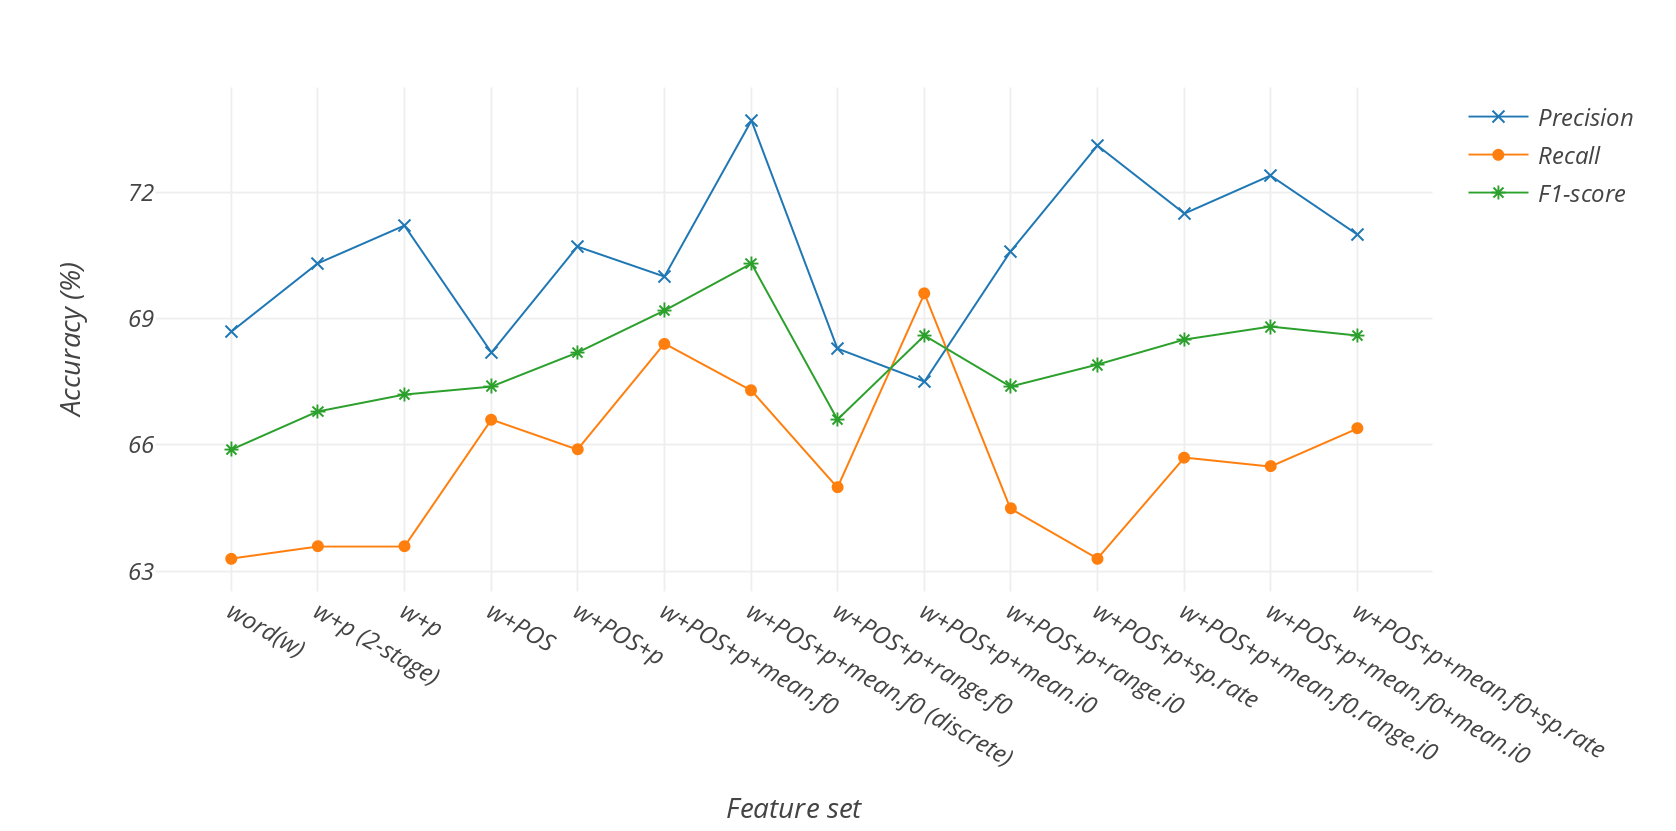
\includegraphics[scale=.99]{img/csl/overall-punk.png}}
\end{minipage}%
\par\medskip
\centering
\subfloat[]{\label{each-punk}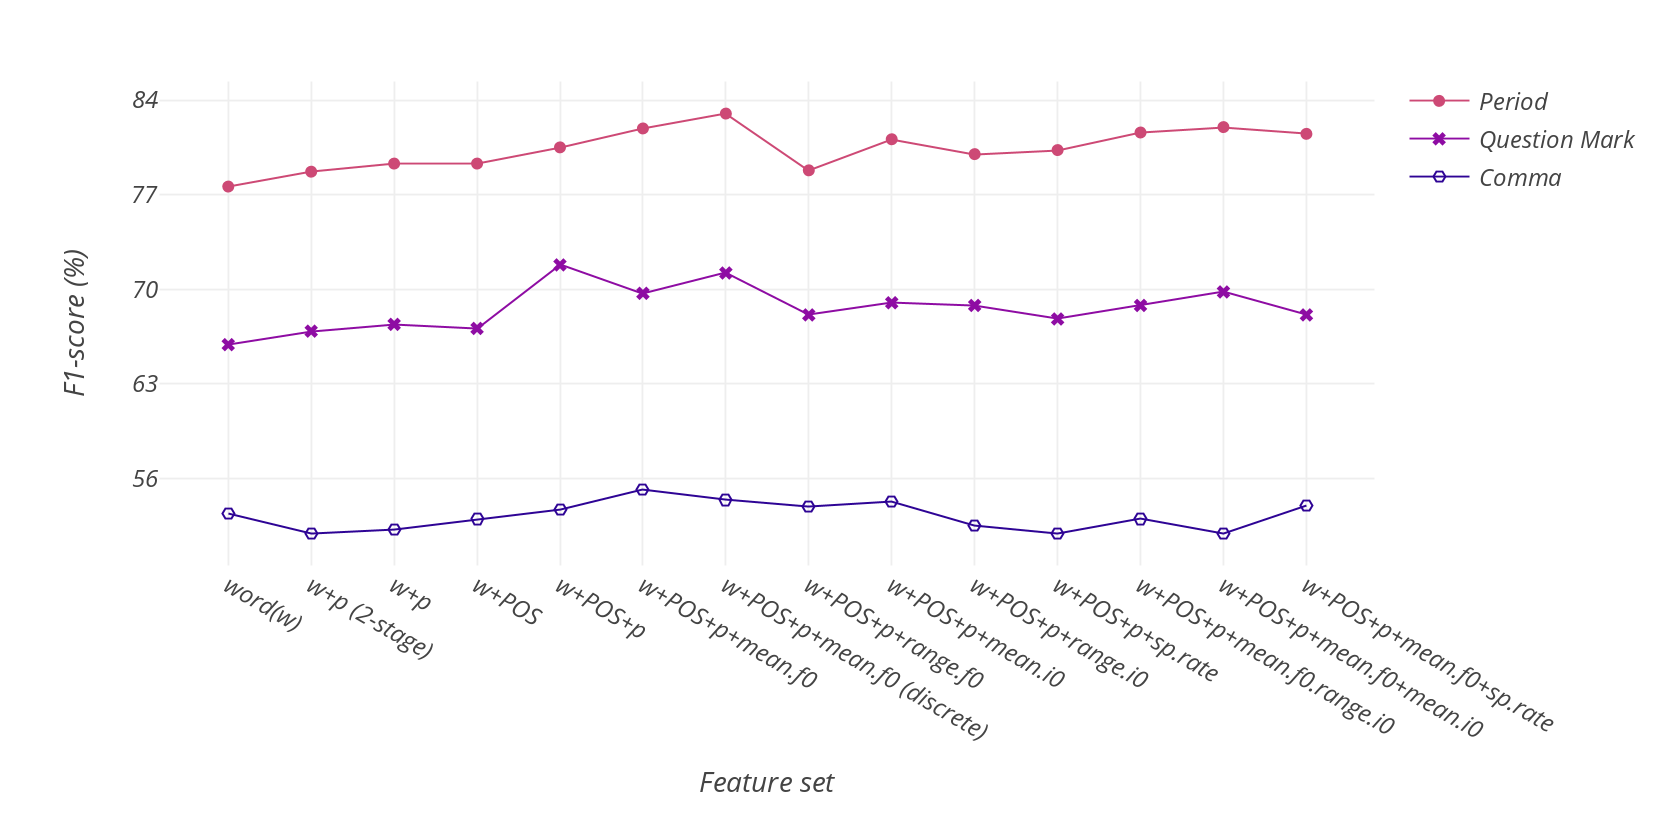
\includegraphics[scale=.99]{img/csl/each-punk.png}}
\caption{(a) Overall punctuation results in terms of precision, recall and $F_1$ score (b) $F_1$ score of each punctuation mark in different feature settings.}
\label{fig:main}
\end{figure}

Table \ref{examples} shows some examples from the testing set punctuated with solely word-based and word-prosody combined model. Listening to the audio samples, one can spot some examples that show improvement caused by prosodic models (sentences 2c and 4c in Table \ref{examples}). 
However, other examples (sentences 1c and 3c in Table \ref{examples}) also show that there are some cases where inclusion of prosodic features do not necessarily help the correct prediction of punctuation. In the case of sentence 1c, the speaker consistently makes pauses after most words and makes prominent most content words. That might be the reason why prosodic features do not help establish the correct punctuation after the word {\it axons}. On the other hand, the sample for sentence 3a points out that the model that includes prosodic features has some limitations as it inserts a comma in the middle of a clearly audible prosodic unit {\it video cassette recorders}. One plausible solution to overcome this limitation may be testing including other features or giving more weight to prosodic features over textual ones.

\begin{table}[tbp]
\centering

\begin{tabular}{p{0.5cm}|l|p{12cm}}
\toprule
ID & Model & Sentence  \\
\midrule
%\multicolumn{2}{l}{Example (1)}\\
1a & Gold & So all of those colored lines correspond to bunches of axons\mycirc{\textbf{,}} the fibers that join cell bodies to synapses\mycirc{\textbf{.}} \\
1b & Word & so all of those colored lines correspond to bunches of axons\mycirc{\textbf{,}} the fibers that join cell bodies to synapses\mycirc{\textbf{.}}  \\ 
1c & W\&Pr & so all of those colored lines correspond to bunches of axons the fibers that join cell bodies to synapses\mycirc{\textbf{.}}  \\
\midrule
%\multicolumn{2}{l}{Example (2)}\\
2a & Gold & Now molecules are really\mycirc{\textbf{,}} really tiny\mycirc{\textbf{.}} \\
2b & Word & now\mycirc{\textbf{,}} molecules are really really tiny\mycirc{\textbf{.}}  \\
2c & W\&Pr & now\mycirc{\textbf{,}} molecules are really\mycirc{\textbf{,}} really tiny\mycirc{\textbf{.}} \\ 
\midrule
%\multicolumn{2}{l}{Example (3)}\\
3a & Gold & Cassette tapes\mycirc{\textbf{,}} video cassette recorders\mycirc{\textbf{,}} even the humble Xerox machine created new opportunities for us to behave in ways that astonished the media business\mycirc{\textbf{.}} \\
3b & Word & cassette tapes\mycirc{\textbf{,}} video cassette recorders\mycirc{\textbf{,}} even the humble xerox machine\mycirc{\textbf{,}} created new opportunities for us to behave in ways that astonished the media business\mycirc{\textbf{.}} \\
3c & W\&Pr & cassette tapes\mycirc{\textbf{,}} video\mycirc{\textbf{,}} cassette recorders\mycirc{\textbf{,}} even the humble xerox machine created new opportunities for us to behave in ways that astonished the media business\mycirc{\textbf{.}}  \\ 
\midrule
%\multicolumn{2}{l}{Example (4)}\\
4a & Gold & And you could see how my poor\mycirc{\textbf{,}} manipulated sister faced conflict\mycirc{\textbf{,}} as her little brain attempted to devote resources to feeling the pain and suffering and surprise she just experienced\mycirc{\textbf{,}} or contemplating her new found identity as a unicorn\mycirc{\textbf{.}} \\
4b & Word & and you could see how my poor manipulated sister faced conflict as her little brain attempted to devote resources to feeling the pain and suffering and surprise\mycirc{\textbf{,}} she just experienced or contemplating her new found identity as a unicorn\mycirc{\textbf{.}} \\ 
4c & W\&Pr & and you could see how my poor manipulated sister faced conflict\mycirc{\textbf{,}} as her little brain attempted to devote resources to feeling the pain and suffering and surprise she just experienced\mycirc{\textbf{,}} or contemplating her new found identity as a unicorn\mycirc{\textbf{.}} \\ \midrule
%\multicolumn{2}{l}{Example (5)}\\
% 5a & Gold & If you do that tomorrow, I'll be dead, you'll be dead, every single one of the men will be dead. \\
% 5b & Word & if you do that tomorrow, i'll be dead, you'll be dead every single one of the men will be dead. \\
% 5c & W\&Pr & if you do that tomorrow, i'll be dead. you'll be dead. every single one of the men will be dead. \\     
\end{tabular}
\caption{Punctuation generation results for a set of sentences. Audio samples can be accessed from the Github repository\footnote{\url{github.com/alpoktem/punkProse/tree/master/audio-samples}}.}
\label{examples}
\end{table}

\subsection{What's the effect of punctuation presence to syntactic parsing?}
\label{punkProse:experiments:q2}
The first step of many NLP applications involves the parsing of an input phrase to the system. In a system with human input for example, it allows further interpretation of the input phrase through a syntactic analysis. The output of a syntactic parser is a \textit{dependency tree}, where the sentence is defined as a group of relations between the elements of a sentence. Figure \ref{punkProse:figure:parsing} illustrates an example of a dependency tree. Most syntactic parsers are statistical in a sense that they determine these relations based on knowledge gained from a huge corpus of hand-annotated dependency trees. Words, as well as punctuation marks are the nodes of dependency trees. 

\begin{figure}[h]
\centering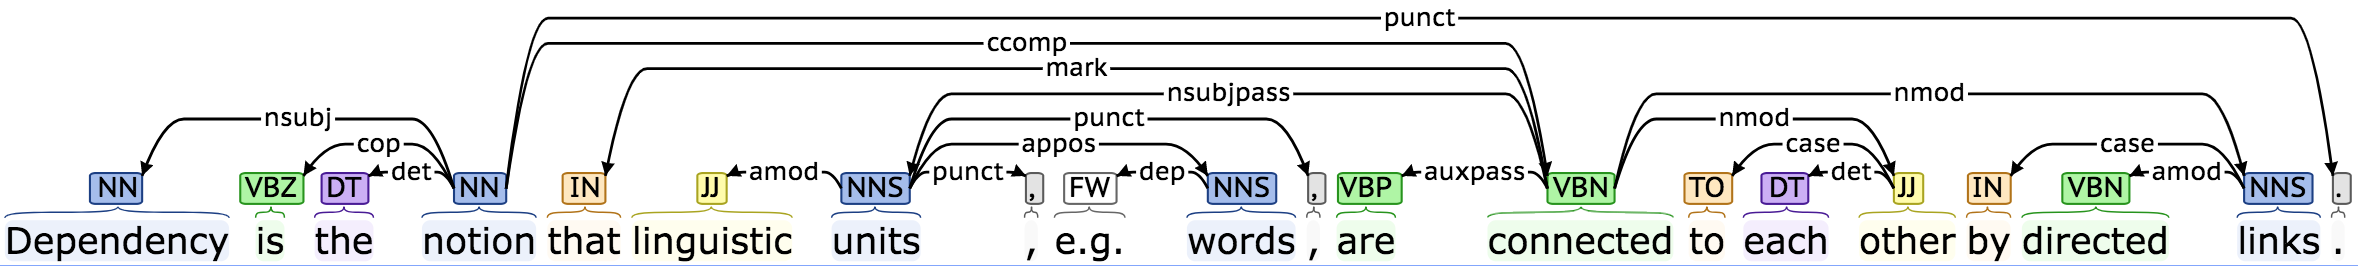
\includegraphics[width=\linewidth]{img/dependency_tree.png}
\caption{An example of a dependency tree generated with an English parser\footnote{\url{http://corenlp.run/}}.}
\label{punkProse:figure:parsing}
\end{figure}

As much as human understanding of written language is affected by it, syntactic parsers also depend on punctuation marks on input sentences \citep{Jones:1994:ERP:991886.991960}. First and most important cue lying in punctuation is the sentence boundaries. Syntactic parsing is generally performed on a sentence. Thus, parsing of huge texts imply segmentation of it from sentence boundaries. Other punctuation marks have also effect on parsing as they are grammatical and semantic elements of a sentence. 

In this section, I will perform an experiment on examining the effect of punctuation placed by the trained prosodic punctuation models on dependency parsing. Specifically, I wanted to examine if the commas predicted with our models help the parsing. As wrong placement of commas could decrease the parser accuracy, I wanted to test if the relatively low-scoring comma prediction helps the parser output. 

\subsubsection*{Experimental setup}

One hundred sentences that represent different types of comma events have been collected from our test set. The collection includes simple to complex sentences with commas used for different functions; e.g., enumeration, dislocation of noun phrases, and clause division, among others. Some sentences in which different placement of commas could lead to different semantic or syntactic structures have also been chosen. 

Sentences with gold punctuation (from original annotations), with punctuation taken out, and with predicted punctuation (with and without prosodic features) were parsed using a state-of-the-art dependency parser \citep{Bohnet:2012:BBW:2380816.2380828,
Bohnet:2012:TSJ:2390948.2391114}. In order to compare the parsing results, the standard dependency parser quality metrics \textit{Unlabeled Attachment Score (UAS)}  and \textit{Labeled Attachment Score (LAS)} are used. For assessing the closeness of two dependency trees, UAS measures the number of arcs with correct head and dependencies. On top of UAS, LAS measures whether the dependency labels are correct \citep{Buchholz:2006:CST:1596276.1596305}. For more information on UAS and LAS refer to \cite{Nivre2017UniversalDE, green:dependency}.

\subsubsection*{Results}

The results listed in Table \ref{parsing} show that dependencies are labeled wrong in 16.6\% of the cases if punctuations are omitted; cf. the corresponding LAS. Labeled dependency trees get more similar to the gold standard with the introduction of commas using our models. Thus, LAS improves by 5\% when only word features and by 5.7\% when both word and prosodic features are used, resulting in a decreased error rate of 10.9\%. A similar tendency can be observed with UAS. The results show that consideration of prosody improves dependency parsing. 

\begin{table}[H]
	\centering
	\begin{tabular}{p{8cm}p{2cm}ccc}
		\toprule
         &  \multicolumn{2}{c}{Similarity}  \\
         Setting   							& LAS   &  UAS  \\
		\midrule
        Unpunctuated 					& 83.4\% & 86.3\% \\
		Punctuated with word feature	& 88.4\% & 89.8\% \\
		Punctuated with word and prosodic features  & 89.1\% & 90.6\% \\
		\bottomrule
	\end{tabular}
	\caption{Parsing similarity results}
	\label{parsing}
\end{table}

\subsection{Performance with ASR output}
\label{punkProse:experiments:q3}
In this section, I further extend on the performance tests by attaching the developed prosodic punctuation restoration models into a speech recognition pipeline. A testing interface is prepared that uses a state-of-the-art ASR system to convert spoken input to raw transcription and \textit{Prosograph} \citep{prosograph} to analyze the input prosody. Punctuation restoration is then performed on the raw transcripts with the two types of models models that were trained during the experiments: Text-only model and best performing text+prosodic model. Through these tests it is possible to see the performance of the proposed methodology on a setting closer to a real-world use case \citep{punkProse}.

\subsubsection{Overview of the testing interface}

The testing interface is designed so that spoken input can be given to the interface either by recording with microphone or by presenting a pre-recorded file which is then sent to an ASR system for transcription. The transcriptions, punctuated with our models, are displayed together with their graphical prosodic visualizations. 

As depicted in Figure \ref{punkProse:figure:testing_system}, the pipeline of the testing interface can be summarized as follows: (1) Obtaining a recording from either microphone or a waveform audio file, (2) transcription using a speech-to-text system\footnote{Google's Cloud ASR service is employed.}, (3) prosodic and syntactic feature extraction, (4) punctuation restoration, (5) visualization of punctuated versions of transcript together with acoustic measurements. See Figure \ref{punkProse:testing_interface} for example of the testing interface. 

\begin{figure*}
\begin{center}
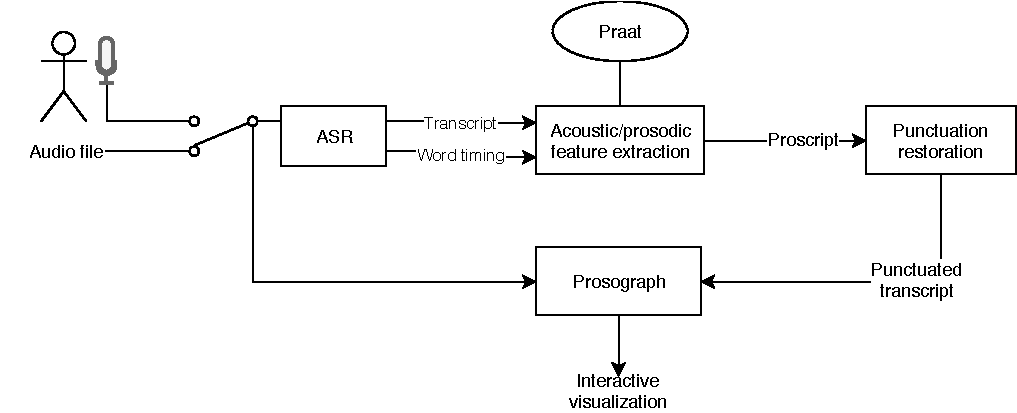
\includegraphics[width=0.7\textwidth]{img/punkProse_setup.pdf}
\caption{Architecture of the interactive ASR testing setup.}
\label{punkProse:figure:testing_system}
\end{center}
\end{figure*}

\begin{figure*}
\begin{center}
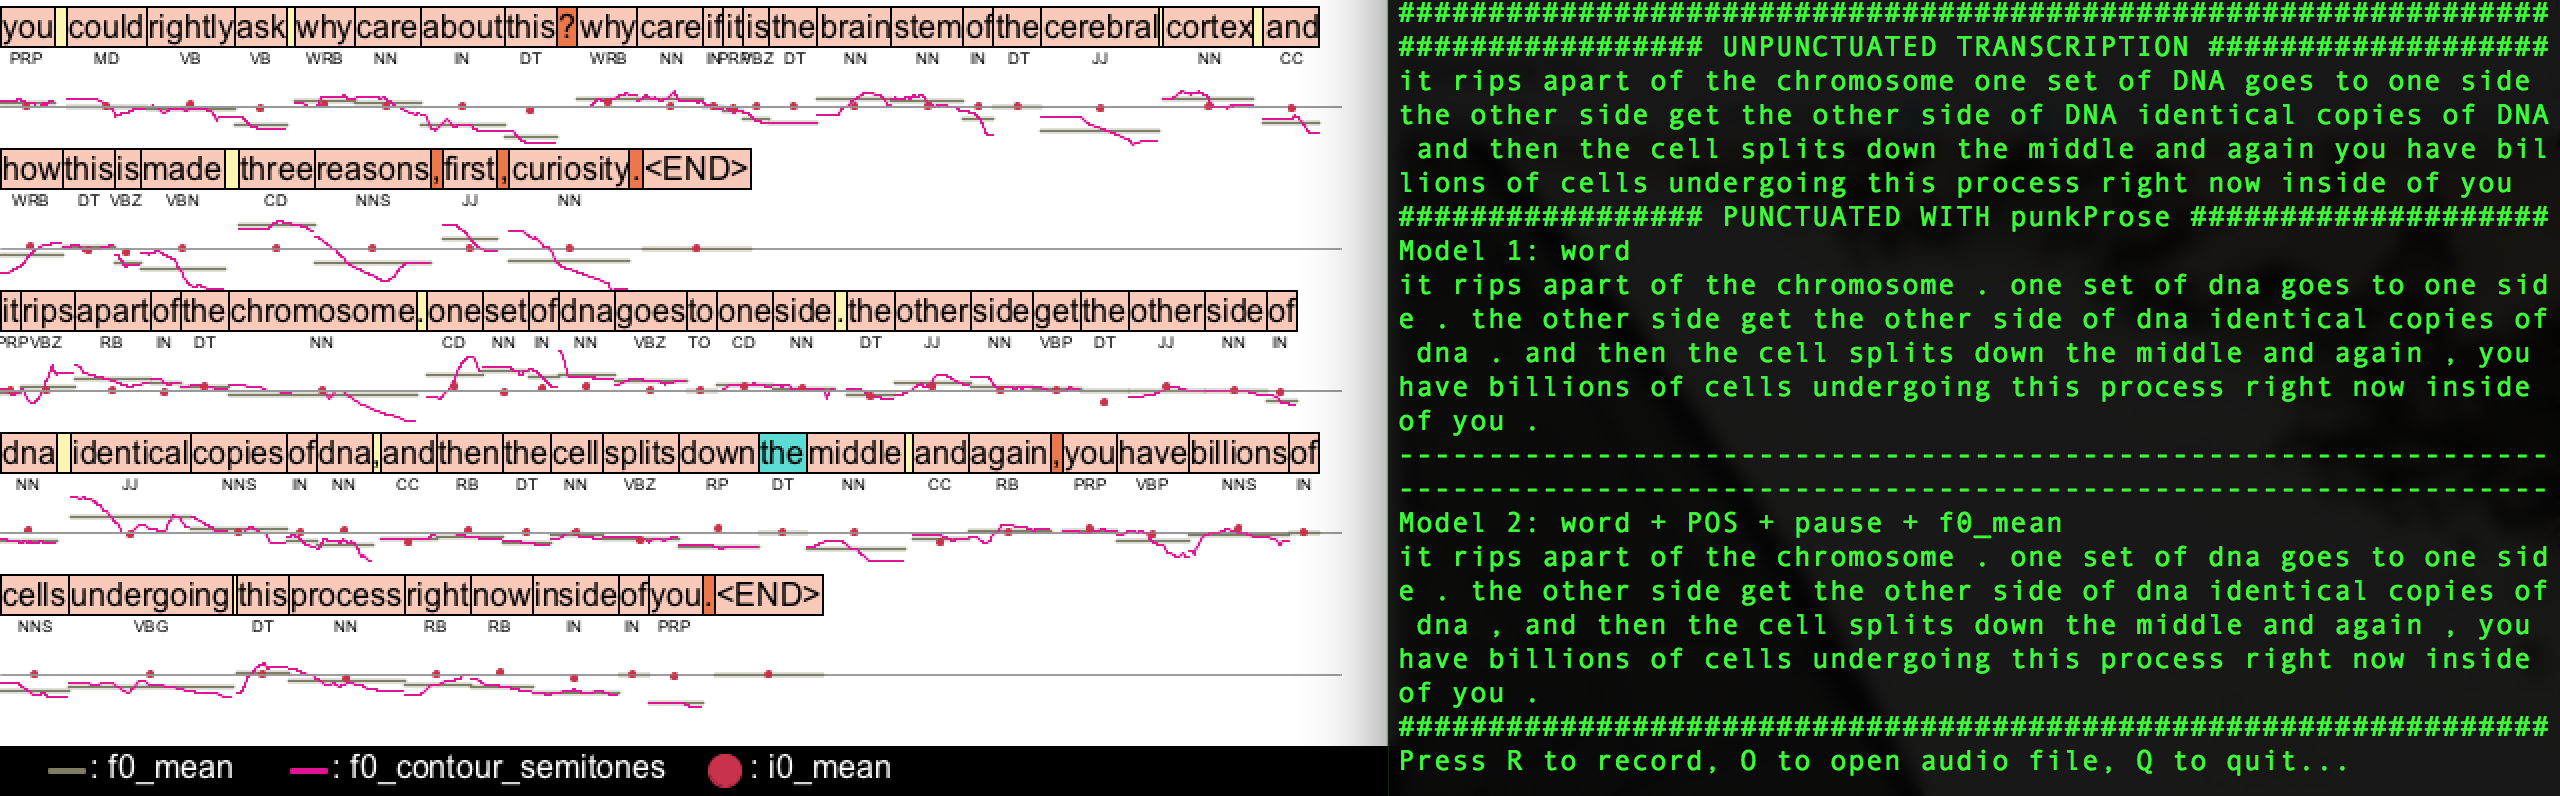
\includegraphics[width=1.0\textwidth]{img/interface-5.png}
\caption{The two window interactive test environment. Recordings are presented through the command line interface (right) and visualized directly on Prosograph (left).}
\label{punkProse:testing_interface}
\end{center}
\end{figure*}

\subsubsection{Selected testing samples}
Here I will show some samples from the Heroes Corpus running through the testing interface. I test on examples from the movie domain to get insight on how the proposed model would work on an automatic captioning use case. 

Figure \ref{figure:heroes_pp_1} shows an example that was recognized well with the ASR system. Both text and prosodic punctuation restoration models perform well in recognizing the sentence boundary. Figure \ref{figure:heroes_pp_2} illustrates an example where the ASR system fails to recognize the speech input accurately. In this example, textual model works better in determining the boundary marked by a comma in the original sentence. Even though the boundary is marked by a long pause, the prosodic model doesn't perform well due to the ungrammatical structure of the recognized utterance. 

Figure \ref{figure:heroes_pp_3} also illustrates a misrecognized example. The tag question ``don't you'' at the end of the speech sample is not recognized. Without that part, the text model marks the sentence end with a period. However, the prosodic model captures the intonation of the sample and predicts successfully the question mark at the end. This example shows that the prosodic model is able to predict well in some cases even though ASR fails to recognize the input speech accurately. 

All in all, the models trained on conference speeches show an acceptable and usable performance on ASR output and on a different domain than the models are trained on. With further domain adaptation better results can be obtained. 

\begin{figure}[h]
    \centering
    \begin{minipage}[t]{0.5\textwidth}
    \begin{tabular}{c}
    \textbf{Original utterance}\\
    I'm so sorry I left you. It wasn't easy for me. \\
    \end{tabular}
    \end{minipage}
    %\hfill
    \\
    \begin{minipage}[t]{0.35\textwidth}
    \begin{tabular}{c}
    \textbf{Prosodic visualization}\\
    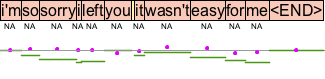
\includegraphics[height=1.5cm]{img/s2_5_0227-EN.png} \\
    \end{tabular}
    \end{minipage}
    \\
    \begin{minipage}[t]{0.5\textwidth}
    \begin{tabular}{c}
    \textbf{Punctuation restored (Word model)}\\
    i'm so sorry i left you. it wasn't easy for me \\
    \end{tabular}
    \end{minipage}
    \\
    \begin{minipage}[t]{0.5\textwidth}
    \begin{tabular}{c}
    \textbf{Punctuation restored (Word+Prosodic model)}\\
    i'm so sorry i left you. it wasn't easy for me \\
    \end{tabular}
    \end{minipage}
    \caption{Segment pair s2\_5\_0227 from the Heroes corpus}
    \label{figure:heroes_pp_1}
\end{figure}
\hfill
\begin{figure}[h]
    \centering
    \begin{minipage}[t]{3.5\textwidth}
    \begin{tabular}{c}
    \textbf{Original utterance}\\
    This American girl, she's hitting all the boys on the dock... looking for a certain shipping container. \\
    \end{tabular}
    \end{minipage}
    %\hfill
    \\
    \begin{minipage}[t]{3\textwidth}
    \begin{tabular}{c}
    \textbf{Original Prosodic visualization}\\
    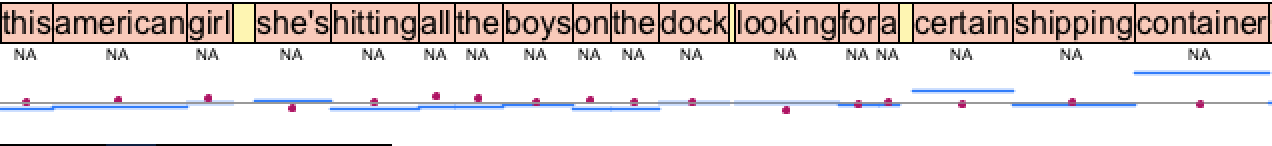
\includegraphics[height=1.5cm]{img/s2_5_0107_asr.png} \\
    \end{tabular}
    \end{minipage}
    \\
    \begin{minipage}[t]{3\textwidth}
    \begin{tabular}{c}
    \textbf{Prosodic visualization of recognized speech}\\
    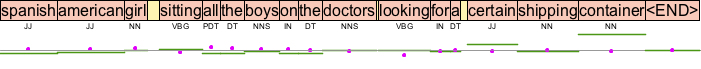
\includegraphics[height=1.5cm]{img/s2_5_0107.png} \\
    \end{tabular}
    \end{minipage}
    \\
    \begin{minipage}[t]{2.2\textwidth}
    \begin{tabular}{c}
    \textbf{Punctuation restored (Word model)}\\
    spanish american girl, sitting all the boys on the doctors looking for a certain shipping container.   \\
    \end{tabular}
    \end{minipage}
    \\
    \begin{minipage}[t]{2.2\textwidth}
    \begin{tabular}{c}
    \textbf{Punctuation restored (Word+Prosodic model)}\\
    spanish american girl sitting all the boys on the doctors looking for a certain shipping container.  \\
    \end{tabular}
    \end{minipage}
    \caption{Segment pair s2\_5\_0107 from the Heroes corpus}
    \label{figure:heroes_pp_2}
\end{figure}
\hfill
\hfill
\begin{figure}[h]
    \centering
    \begin{minipage}[t]{0.5\textwidth}
    \begin{tabular}{c}
    \textbf{Original utterance}\\
    You care about her, don't you? \\
    \end{tabular}
    \end{minipage}
    %\hfill
    \\
    \begin{minipage}[t]{0.5\textwidth}
    \begin{tabular}{c}
    \textbf{Original Prosodic visualization}\\
    \includegraphics[height=1.5cm]{img/s2_5_0114.png} \\
    \end{tabular}
    \end{minipage}
    \\
    \begin{minipage}[t]{0.5\textwidth}
    \begin{tabular}{c}
    \textbf{Prosodic visualization of recognized speech}\\
    \includegraphics[height=1.5cm]{img/s2_5_0114_asr.png} \\
    \end{tabular}
    \end{minipage}
    \\
    \begin{minipage}[t]{0.5\textwidth}
    \begin{tabular}{c}
    \textbf{Punctuation restored (Word model)}\\
    you care about it .  \\
    \end{tabular}
    \end{minipage}
    \\
    \begin{minipage}[t]{0.5\textwidth}
    \begin{tabular}{c}
    \textbf{Punctuation restored (Word+Prosodic model)}\\
    you care about it ? \\
    \end{tabular}
    \end{minipage}
    
    \caption{Segment pair s2\_5\_0114 from the Heroes corpus}
    \label{figure:heroes_pp_3}
\end{figure}

\section{Conclusion}
\label{punkProse:discussion}
%TODO: review
In this chapter, I have presented a recurrent neural network architecture that processes lexical and prosodic information in parallel for the generation of punctuation in speech transcripts, avoiding the dominance of written data, and thus the bias of trained models towards written material. The proposed model allows the integration of any desired feature (lexical, syntactic or prosodic) and thus a further analysis of the impact of every feature used on the punctuation generation. In addition, the current model achieves a significant improvement over previous works that used two stages and were biased to written data. An overall $F_1$ score of 70.3\% is reported for comma, period and question mark generation in the used dataset. 

%3. Conclusions on the prosodic features tested so far

The results are shown to be significantly better when syntactic and prosodic features are added to the lexical information. Solely pauses ---when trained with a separate RNN --- improve considerably the vocabulary-based scores. Moreover, f0- and intensity-based prosodic features help to achieve a better comma and period detection in terms of $F_1$ measure. All in all, the best combination of prosodic features is when the model is trained on words, their POS tags together with the preceding pause durations and their normalized mean f0 values. 

Further experiments have been carried out to test the performance of the models on parsing and ASR output. Quantitative metrics on parsing of single sentences showed that prosodic models perform better in obtaining correct dependency trees with syntactic parsing. On a demonstrative setting where ASR was employed, reasonable performance is recorded in recovering punctuation marks on out-of-domain spoken input. Through further model adaptation (e.g. vocabulary extension and speaker adaptation) better results can be obtained.

%TODO: add this
%Effect of prosody in punctuation restoration modelling was tested on two subsequent processes: dependency parsing and machine translation. The former evaluation was conducted on a small dataset and showed that accounting of prosody does imply an improvement in correct paring of the sentences. This shows that commas which are detected more accurately with prosodic models does improve parsing despite its low F-score.

%TODO: Commalarin boktan olmasi buyuk ihtimalle annotationdaki farkliliklarda yatiyor. Comma en az aggree olan punc. 
\newpage\leavevmode\thispagestyle{empty}\newpage
% ---------------------------------------------------------------------

% CHAPTER 5: Translation works
% ---------------------------------------------------------------------
\chapter{Enhancing Spoken Language Translation with Prosody}
\label{chapter:transProse}
This chapter explores around the question of how can prosody be utilized in the framework of spoken language machine translation (SLMT). The first goal of this chapter is to gain insights and prove that prosody is an essential element to consider in spoken language translation. This is performed through linguistic and corpus-based analysis on the bilingual speech corpus that we collected (Section \ref{transProse:analysis}). Following, building of a neural machine translation system is explained in Section \ref{transProse:methodology}. This system serves both as a text translation baseline and a basis for incorporation of prosodic features in both input and output. Next, I perform experiments that utilize this system on the movie-domain translation (speech-to-text and speech-to-speech). First, I explore the effect of prosodic punctuation restoration as a preliminary step to translation in Section \ref{transProse:Q1}. Secondly in Section \ref{transProse:Q2} I aim to improve text translation system through prosodically-enhanced input. And finally, for the aim of generating prosodic synthesis cues in a speech-to-speech translation system, I report on the experiments building a translator that can handle prosodic input and output (Section \ref{transProse:Q3}). 

\section{Motivation and Background}
%introduction and problems faced
Spoken language machine translation is a type of machine translation where input and/or output to the system is spoken language. It is usually used in the context of translating from speech to text (through incorporation of ASR), or speech to speech (through incorporation of ASR and TTS). The MT modules in these systems are designed the same way as standard text translation systems. However, spoken language processing introduces its distinct challenges. For instance, in a system with speech input, the output of ASR lacks punctuation, which provides both linguistic and functional cues for translation. In the case of a spoken input and output system, through a basic concatenation of ASR, MT and TTS systems, prosodic information of the input speech is lost already in the first step. Thus, any communicative information residing in the input speech through prosody is not reflected in the translated and synthesized speech. 

%dubbing vs translation analogy
One can draw an analogy of the difference between spoken language translation and written language translation as the difference between book translation and movie dubbing. A book translator translates a book chapter by chapter, then paragraph by paragraph, and then sentence by sentence. All these segmentations are cued through the layout of the book, paragraph breaks and punctuation. Once at a certain sentence, the translator interprets the sentence in the original language of the book and then transforms it into the translation language following author's intentions. 

Although essentially a translation task, the art of dubbing a movie requires many more challenges. A similar segmentation process is followed but this time through scene information and actor turns. Once a line of an actor is transcripted, it can be segmented into sentences by looking both at grammatical and auditory aspects. The lines are then translated into the dubbing language by translators with the paralinguistic information such as the tone, intention and intensity noted. Finally, the voice actors vocalize these translations respecting these paralinguistic aspects in the original language of the movie. 

%connecting analogy to the technological need
The additional tasks involved in the latter process should somehow be considered in an automatic translation/dubbing system of audiovisual content in order to obtain optimal results. The segmentation part requires tasks such as speech activity detection, speaker turn detection and ASR. The work in this chapter assumes that these tasks are already done perfectly and focuses on the translation part of the system and especially on the involvement of prosody to it. 

Specifically, I will address these three principal questions that involve prosody in the spoken language translation framework:

\begin{enumerate}
    \item How does prosodic punctuation restoration affect translation?
    \item Does pause encoding improve translation?
    \item Can we transfer pausing in speech-to-speech translation?
\end{enumerate}

Before I embark on answering these questions, I will try to give the context to them with a linguistic and corpus study. This study is designed both to inspire the design of a prosodically enhanced translation model and also to help interpret experimental results. The questions will be answered with a practical methodology. A prosodically enhanced translation model needs to be designed and then configured to suit the needs defined by the questions. Through this study, I aim to prove the need for inclusion of prosody in spoken machine translation pipelines and also to introduce a framework that would allow experimentation in this respect. 

\section{Analyzing Significance of Prosody in Machine Translation}
\label{transProse:analysis}
In this section, I perform some example-based and statistical analysis on bilingual segments of the \textit{Heroes corpus}, which was presented in Chapter \ref{chapter:corpusWorks}. This corpus contains parallel English and Spanish speech segments from a dubbed TV series. The aim is to show how prosody is reflected in dubbing translation. Particularly, I focus on pauses as a prosodic feature. The first part demonstrates on a few examples in the corpus how pausing information influences translation, both for text and audio output. In the second part, I follow a more statistical approach to prove significance of pausing in spoken translation. 

\subsection{Example-based Analysis}
\label{subsection:heroes_examples}
In order to gain linguistic insights before building a data-driven model, selected parallel segments from the Heroes corpus are carefully inspected. Specifically, two phenomena are investigated in terms of spoken language translation: How does pausing as a prosodic feature reflects (1) in the translation script and (2) in dubbing (translated voiceover on actor's lip movements). These are then compared to how a classic automated model (machine translation and text-to-speech respectively) performs with same input sentence. All spoken samples presented throughout this chapter can be found in the thesis repository \footnote{\url{https://github.com/alpoktem/PhDThesis}}.

\subsubsection{Indirect transfer of pauses}

I will firstly examine the sample \textit{s2\_5\_0043} from the Heroes corpus. The original punctuated transcription of the English segment is: \textit{He pushed his way in, shoved a gun in my face. Next thing I know, he's flying through that glass.} Figure \ref{figure:heroes_viz_1} shows the Prosograph visualization of English and Spanish version of the sample. Yellow boxes indicate paused intervals between words.

%sample 1 - he pushed is way in. 
\begin{figure}[h!]
\begin{minipage}{\textwidth}
\begin{tabular}{c}
ENG \\
\includegraphics[height=1.2cm, width=\textwidth]{img/s2_5_0043-EN.png} \\
\end{tabular}
\end{minipage}
%\hfill
\begin{minipage}{\textwidth}
\begin{tabular}{c}
SPA \\
\includegraphics[width=\textwidth]{img/s2_5_0043-ES.png} \\
\end{tabular}
\end{minipage}
\caption{Segment pair s2\_5\_0043 from the Heroes corpus}
\label{figure:heroes_viz_1}
\end{figure}

Both segments are formed of 4 clauses. English segment consists of two sentences whereas in the Spanish segment these two sentences are joined with a linking word \textit{"y"} (and). Pauses are observed in all clause boundaries in English segment, whereas in the Spanish segment, a clause boundary pause is observed only after \textit{"de repente"} (\textit{lit.} suddenly, non-literal translation of \textit{"next thing I know"}. 

A fairly longer non-clause boundary pause is observed at the beginning of both sentences. 0.25 seconds of pause are observed after \textit{"he"} in English and 0.31 seconds of pause are observed after \textit{"ha"} (part of a compound verb to mark past tense) in Spanish. In the last clause in English, two short pauses are observed, which is not reflected in the Spanish sentence. However, when we listen to the Spanish segment, instead of a pause, a lengthening of the word \textit{"ha"} is observed. 

With a focus on pauses, we can make the following observations with respect to prosodic realizations in this particular segment pair:
\begin{enumerate}
    \item Pauses are not necessarily reflected in translation, even though they are induced by grammatical structures like clauses.
    \item Even though pauses can be reflected with respect to their position in a sentence, they can come in between different words that do not necessarily correspond. 
    \item A prosodic phenomena can be expressed in different ways, e.g. by lengthening a word. 
\end{enumerate}
%TODO: \mireia{I found this paper https://core.ac.uk/download/pdf/84560.pdf  that could be relevant here. Or maybe worth citing it the state of the art.}

This parallel segment shows the complexity of the problem of prosodic transfer. It is hard to predict the prosodic realizations of the translation of a sentence only by looking at prosodic features in the input sentence. It is assumed that the English and Spanish versions of the segment are expressed in a similar fashion by the two actors, explaining these particular prosodic reflections. However, another voice actor could possibly dub this line in a different way with a different prosodic structure as well.  

%translation experiments
Next, a state of the art machine translation system is employed to see its performance in translating the this example. Translations are performed using a state-of-the-art commercial neural network based translator\footnote{Google Translate: \url{translate.google.com}}.  

\begin{description}
\item [Input sentence (ENG)] {\it He pushed his way in, shoved a gun in my face. Next thing I know, he's flying through that glass.}
\item [MT (ENG $\rightarrow$ SPA)] {\it Se abrió paso empujándome una pistola en la cara. Lo siguiente que sé es que está volando a través de ese cristal.}
\end{description}

What is noticed first is the mistranslations of some parts of the phrase. However, it is not our point to assess the quality of the translation in terms of correct word usage. The translated phrase represents the actions and objects in the source sentence well enough for our study. 

It is examined that the first two clauses in the English phrase are joined into one: \textit{Se abrió paso empujándome una pistola en la cara} (lit. \textit{He opened the way pushing a gun in my face}). Even though there is a comma separating the two clauses explicitly in the input sentence, this is not reflected in the translation. When we translate this section with punctuation marks removed we get a similar result:

\begin{description}
\item [Input sentence (ENG)] {\it he pushed his way in shoved a gun in my face} 
\item [MT (ENG $\rightarrow$ SPA)] {\it él se abrió paso empujándome una pistola en la cara}
\end{description}

The phrase, both prosodically and gramatically, is structured in a way that the speaker is explaining a sequence of actions: character pushing in and then pointing a gun on the speaker. Even though this is cued orthographically through punctuation, still the translation system is not able to capture this structure. An ideal translation that takes heed of the prosodic structure would be:
\textit{Él se abrió paso, empujó una pistola en mi cara. Lo siguiente que sé, él está volando a través de ese cristal.}\footnote{Only changing the structure respecting how the translator performs.} This example shows that a translation system that disregards the prosodic structure of the source sentence fails to translate in a way that was originally uttered. 

\subsubsection{Direct transfer of pauses}
Next, I will list some examples where pausing is somewhat more directly transferred between original and dubbing language. Many samples of this type were found in the corpus. Three samples are demonstrated in Figures \ref{figure:heroes_viz_2} to \ref{figure:heroes_viz_4}. 

%this here's everything you had on you
\begin{figure}[h!]
\centering
\begin{minipage}[t]{0.61\textwidth}
\begin{tabular}{c}
ENG \\
\includegraphics[height=1.2cm]{img/s2_5_0010-EN.png} \\
\end{tabular}
\end{minipage}
%\hfill
\\
\begin{minipage}[t]{0.4\textwidth}
\begin{tabular}{c}
SPA \\
\includegraphics[height=1.2cm]{img/s2_5_0010-ES.png} \\
\end{tabular}
\end{minipage}
\caption{Segment pair s2\_5\_0010 from the Heroes corpus}
\label{figure:heroes_viz_2}
\end{figure}

\begin{figure}[h!]
\centering
\begin{minipage}[t]{0.63\textwidth}
\begin{tabular}{c}
ENG \\
\includegraphics[height=1.2cm]{img/s2_5_0020-EN.png} \\
\end{tabular}
\end{minipage}
%\hfill
\\
\begin{minipage}[t]{0.85\textwidth}
\begin{tabular}{c}
SPA \\
\includegraphics[height=1.2cm]{img/s2_5_0020-ES.png} \\
\end{tabular}
\end{minipage}
\caption{Segment pair s2\_5\_0020 from the Heroes corpus}
\label{figure:heroes_viz_3}
\end{figure}

\begin{figure}[h!]
\centering
\begin{minipage}[t]{0.37\textwidth}
\begin{tabular}{c}
ENG \\
\includegraphics[height=1.2cm]{img/s2_5_0050-EN.png} \\
\end{tabular}
\end{minipage}
%\hfill
\\
\begin{minipage}[t]{0.4\textwidth}
\begin{tabular}{c}
SPA \\
\includegraphics[height=1.2cm]{img/s2_5_0050-ES.png} \\
\end{tabular}
\end{minipage}
\caption{Segment pair s2\_5\_0050 from the Heroes corpus}
\label{figure:heroes_viz_4}
\end{figure}

Pause intervals can be directly traced at the phrase boundaries in both languages. These samples suggest a simpler approach in transfer of pauses. Also, it is observed in most of the examples of this type that the slot where the pause occurs is marked with a punctuation. However, in order to arrive to more concrete conclusions on direct pause transfer and punctuation co-occurrence, a statistical study is conducted in the next subsection. 
 
\subsection{Corpus-driven analysis}

Manual analyses done in the previous subsection are further extended to get a generalized view of the Heroes corpus on pausing. The motivation behind this study is to first, evaluate statistically how pausing is reflected in the dubbing translations, and second, how much pausing is related to punctuation. 

\subsubsection{How pausing is reflected in translation?}
A straightforward scheme is followed to evaluate how much of the pause events in English segments are reflected in the Spanish segments. A segment with a pause event means that there is one or more inter-word interval with a pausing of minimum 0.05 seconds of duration. To quantify this in the Heroes parallel corpus, first, number of segments with a pause event is counted for both English and Spanish segments. Then, number of segment pairs that contain a pause event only in English, only in Spanish and both in English and Spanish is calculated. See Table \ref{table:pausing} for the results. 

%pausing
\begin{table}[ht]
\centering
\begin{tabular}{>{\centering\arraybackslash} m{0.48\linewidth} >{\centering\arraybackslash} m{0.3\linewidth} }
\hline
 & \textbf{\# Segments} \\ \hline
\textit{Pause in English segment} &  3050 \\
\textit{Pause in Spanish segment} & 3493  \\
\textit{Pause in both English and Spanish} & 2539  \\ 
\textit{Pause only in English segment} & 511  \\
\textit{Pause only in Spanish segment} & 954  \\ \hline
\end{tabular}
\caption{\label{table:pausing}Shared pause events in English and Spanish segments of the Heroes corpus. }
\end{table}

It can be seen that in 83\% of the cases, a pause event in English segment is reflected in the Spanish segment. Other way around, in 72\% of the cases, a pause event in Spanish segment is reflected in the English segment. It can be deduced that pausing as a prosodic feature is reflected in the dubbing translations in majority of the cases. In this study, positions of the pauses are ignored. 

\subsubsection{To what extend pausing is associated with punctuation in subtitle transcripts?}

In the manual inspections performed in Subsection \ref{subsection:heroes_examples}, it was observed that many times pauses occur at punctuated slots between words in the subtitle transcription. Below, I explore this on a statistical basis in English segments of the Heroes corpus. The importance of this study is to know how much pausing influence punctuation placement and vice versa. Two directions of co-occurrence are observed: (1) how is a paused interval punctuated? and (2) to what extend punctuation infers a paused interval? I answer the first question in Figure \ref{figure:if_pause_then_punctuation} where distribution of punctuation events in paused intervals is shown. In English segments, among 1854 inter-word slots with a pausing, 80\% of them are annotated with a punctuation in the subtitle transcripts. The majority of the punctuation marks at these paused intervals are sentence ending punctuation marks (period [.], question mark [?], exclamation mark [!]), whereas comma [,] and ellipsis [...] consist of a smaller percentage. Spanish segments demonstrate a similar behaviour in terms of the ratio of punctuated slots with 78\% of them annotated with a punctuation mark. Whereas it is observed that commas tend to be paused more compared to English. 

\begin{figure}[h]
    \centering
    \begin{minipage}{.5\textwidth}
        \centering
        \includegraphics[width=\linewidth]{img/if_pause_then_punctuation_ENG.png}
    \end{minipage}%
    \begin{minipage}{0.5\textwidth}
        \centering
        \includegraphics[width=\linewidth]{img/if_pause_then_punctuation_SPA.png}
    \end{minipage}
    \begin{minipage}{.5\textwidth}
        \centering
        English
    \end{minipage}%
    \begin{minipage}{0.5\textwidth}
        \centering
        Spanish
    \end{minipage}
\label{figure:if_pause_then_punctuation}
\caption{Punctuation distribution at paused ($ > 0.05$ s) intervals in English segments(1936 in total) of the Heroes corpus.}
\end{figure}

Secondly, Table \ref{table:if_punctuation_then_pause} shows the distribution of pausing events at inter-word intervals where a punctuation occurs. Looking at English segments, when all punctuation marks are considered, there is a pause in that interval with a 58\% of probability. However, when only sentence ending punctuation marks are considered this percentage rises to 75\%. It can be deduced that a sentence boundary is a highly discriminating cue for a pausing event between two words. However, the ratio of pause presence at occurrences of comma is quite low (39\%). Whereas in Spanish segments, commas seem to be paused much more with a 60\% of them marking a short pause of 420 ms in average. Punctuation marks that act as a sentence boundary also mark a pause more than in English segments (86\%). Both these contribute to a higher distribution of pausing at punctuation points. 72\% of punctuation marks are paused, which is 14\% higher than in English segments. 

Through these studies it can be confirmed that pausing is a highly correlated phenomena with punctuation. And as much as punctuation acts as an important cue in machine translation, pauses can also have a similar role through complementing punctuation or acting as a sole feature in absence of one. 

%if_punctuation_then_pause table
\begin{table}[ht]
\centering
\begin{tabular}{>{\centering\arraybackslash} m{0.25\linewidth} >{\centering\arraybackslash} m{0.16\linewidth} >{\centering\arraybackslash} m{0.16\linewidth} >{\centering\arraybackslash} m{0.14\linewidth} >{\centering\arraybackslash} m{0.16\linewidth}}
 & \textbf{\#Occurrences} & \textbf{\#Occurrences w/ pause} & \textbf{Percentage of paused} & \textbf{Mean pause duration (s)}\\ \hline
\textbf{English} & & & & \\
 \hline
\textit{Punctuated interval}      &  5429 & 3152 & 58 & 0.81 s\\
\textit{Sentence boundary}        &  2549  & 1913 & 75 & 1.02 s\\
\textit{Comma}                    &  2652 & 1038 & 39 & 0.38 s \\ 
\textit{Ellipsis}                 &  228 & 201 & 88 &0.94 s\\ \hline
\textbf{Spanish} & & & & \\
 \hline
\textit{Punctuated interval}      &  4935 & 3580 & 72 & 0.77\\
\textit{Sentence boundary}        &  1856  & 1606 & 86 & 1.11\\
\textit{Comma}                    &  2718 & 1653 & 60 & 0.42  \\ 
\textit{Ellipsis}                 &  361 & 321 & 88 &0.83 s\\ \hline
\end{tabular}
\caption{\label{table:if_punctuation_then_pause}Pause presence in punctuated intervals in English and Spanish segments of Heroes corpus.}
\end{table}

\section{Methodology}
\label{transProse:methodology}

Having the intuition gained from examining prosodic parallelisms in the bilingual segments of the Heroes corpus, I embark on building a system that can learn and generate prosodic structures in a neural machine translation setting. This section explains the framework built in order to carry out experiments to answer the questions we listed earlier. Before diving in the technical specifications of the system built, I will list the requirements defined prior to the implementations:

\begin{enumerate}
    \item Translation will be in movie domain. This is mainly because of our motivation for gaining insights for the automatic subtitling and dubbing use cases. 
    \item System will be extended incrementally i.e.~we will start from a basic text translation system and then add on it first prosodic input and then prosodic output. 
    \item Prosodic encoding and decoding will be built within the translation systeml; i.e.,~text and prosodic encoding and decoding parameters will be learned jointly. 
    \item The system should be able to compensate for the scarcity of spoken parallel data. 
\end{enumerate}

In order to address these requirements, a system is built that can learn translation of textual and prosodic features. I will refer to this system as \textit{TransProse} for simplicity. Design and subtleties of this model are explained in the next subsection \ref{transProse:methodology:model}. Next, data sources that suit best for our problem has to be selected. Collected and acquired corpora and our preprocessing steps are detailed in subsection \ref{transProse:methodology:data}. 

\subsection{Neural Translation Model}
\label{transProse:methodology:model}

%TODO: Citations missing here
Sequence-to-sequence modeling has proved in recent years that it is one of the most advanced models for modelling automatic translation. This model works by \textit{encoding} a phrase in the source language to a single vector and then \textit{decoding} it into the phrase in the target language. A drawback of this classic encoder-decoder architecture is that the entire encoded sequence has to go through one vector acting as a funnel to be decoded into target sequence. This problem was addressed by the introduction of attention mechanism \citep{bahdanau, luong}, which lets the decoded sequence to focus on relevant areas of the encoded sequence.

TransProse framework is based on a sequence-to-sequence network with attention mechanism, which was explained earlier in Chapter \ref{chapter:sota}. For that reason, I will not go deep into the core of the architecture but I will explain more how it was extended to handle prosodic input and output. 
\subsubsection{Encoding text tokens and prosody}

\begin{figure}
\centering
\includegraphics[width=0.7\linewidth]{img/TransProse_Encoder.pdf}
\caption{TransProse sequence-to-sequence translation encoder with prosodic input.}
\label{figure:transprose_encoder}
\end{figure}

The encoder of the system is illustrated in Figure \ref{figure:transprose_encoder}. The text encoder part (inner box) takes word token indexes as input and passes them through an embedded layer then a linear layer to obtain word vectors of size $H$. Then, this vector is passed to a bidirectional GRU layer, outputting hidden and an output vectors in both directions at each step. The forward and backward output vectors are then summed in order to obtain an output of size $H$ for each input token. 

Encoding jointly with the added prosodic features is depicted in the outer box of the same figure. Note that prosody input vector carries any number of prosodic/acoustic features that belong to the word token at that timestep. This number is denoted with $P$. A separate encoding sequence is followed by the prosodic features. The input features are converted to a vector of size $H$ in a gradual fashion where a linear layer is followed by a non-linearity at each step. Once it is the same size of the GRU input layer, it is summed with the encoded word input and introduced to the bidirectional layer together with the input word token representation. Output vectors at each timestep are then passed on through the decoder. 

\subsubsection{Decoding text tokens and prosody}

\begin{figure}
\includegraphics[width=\linewidth]{img/TransProse_Decoder.pdf}
\caption{TransProse sequence-to-sequence translation decoder with prosodic output.}
\label{figure:transprose_decoder}
\end{figure}

As illustrated in Figure \ref{figure:transprose_decoder}, the decoder is also designed to output either text tokens only or accompanied with their corresponding prosodic features. During training, target sequence tokens are input and passed through first, the embedding layer, then a linear layer followed by a dropout layer until it reaches the GRU layer. The output of the GRU layer is used to determine the attention weights according to each of the effect of the encoder output effect on that particular target token. The attention model is based on the global attention model in \cite{luong}. The weights vector for output at timestep $t$ is calculated as in Equation \ref{equation:attn1}, where $h _ { t }$ stands for GRU output in decoder side and $h _ { s }$ on the target side. General scoring function is used as the scoring function (Equation \ref{equation:attn2}). A general overview of the implementation of the neural attention architecture is illustrated in Figure \ref{figure:transprose_attn}.

\begin{equation}
\label{equation:attn1}
a _ { t } ( s ) = \operatorname { align } \left( h _ { t } , \overline { h } _ { s } \right) = \frac { \exp \left( \operatorname { score } \left( h _ { t } , \overline { h } _ { s } \right) \right) } { \sum _ { s } \exp \left( \operatorname { score } \left( h _ { t } , \overline { h } _ { s } \right) \right) }
\end{equation}
 

\begin{equation}
\label{equation:attn2}
\operatorname { score } \left( h _ { t } , \overline { h } _ { s } \right) = h _ { t } ^ { \top } \mathbf { W } _ { a } \overline { h } _ { s }
\end{equation}

\begin{figure}
\centering
\includegraphics[width=0.7\linewidth]{img/TransProse_attn.pdf}
\caption{Attention mechanism in the TransProse decoder.}
\label{figure:transprose_attn}
\end{figure}

After the attention weights are calculated, encoder outputs are multiplied with these weights and averaged to obtain the context vector. Context vector is then concatenated with the decoder GRU output and eventually used to calculate the vocabulary sized one-hot word token output. 

The depiction of the decoder illustrated in Figure \ref{figure:transprose_decoder} has two types of prosodic outputs: flag and pause value output. Both are predicted with respect to the word output and hidden vector of the GRU layer. Flag outputs are of size 2 and real valued outputs are of size 1. 

The two types of outputs are placed for illustration purposes. The model can be configured to output any number of flag or value type features. 

\subsubsection{Learning procedure}
%Two stage training and parameter loading
A translation model enhanced with prosodic input and/or output is obtained in two stages. First, training is performed on parallel text data updating only the parameters belonging to the text encoder and decoder. On a second stage, training is performed on prosodically annotated parallel data with the joint text+prosody encoder/decoder components. Before starting the second stage training, the extended text+prosodic architecture is initialized with the pre-trained first stage parameters. While training on prosodic data, all parameters are updated, where prosodic model components are trained from scratch. 

%Objective functions
In order to calculate gradients for the model to converge while training, loss functions has to be defined for the model outputs. The loss function compares the prediction of the model to the gold output and back-propagates to decide how the model parameters should be updated. For text token and flag-based outputs, masked cross entropy is used. Whereas for real valued outputs mean square error is employed. The total loss of the system is calculated after each batch by summing each individual loss with its respective weight, as in Equation \ref{equation:loss}:

\begin{equation}
    \label{equation:loss}
    { L }_{ total }= { W }_{ word }\cdot { L }_{ word }+ { W }_{ pauseflag }\cdot { L }_{ pauseflag } + { W }_{ pausevalue }\cdot { L }_{ pausevalue }
\end{equation}

In text training, total loss function is only the loss coming from word token predictions. In audio training, ${ W }_{ word }$ is set to $1.0$ and prosodic feature losses (${ W }_{ pausevalue }$ and ${ W }_{ pauseflag }$) are set to $10.0$. In this work, only pause flag output is employed in the experiment reported in Section \ref{transProse:Q3}. For parameter optimization, Adam algorithm (\cite{DBLP:journals/corr/KingmaB14}) is used. After each training epoch, model is validated on a smaller validation set. Training is continued until no improvement is noted in terms of total loss in the validation set in the last three epochs. 

\subsection{Data and data preprocessing}
\label{transProse:methodology:data}

Training is performed in two stages with two types of data, a parallel text corpus and a prosodically annotated parallel spoken audio corpus. \textit{OpenSubtitles corpus} and \textit{Heroes corpus} were used respectively for the two stages of the task. 

\subsubsection{Parallel text dataset}
In order to keep consistent in the movie domain, text data are also obtained from movie based resources. \textit{OpenSubtitles} collection\footnote{\url{http://www.opensubtitles.org/}} provides parallel text obtained from movie and series subtitles (\cite{Lison2016OpenSubtitles2016EL}). The \textit{OpenSubtitles2018} release\footnote{\url{http://opus.nlpl.eu/OpenSubtitles2018.php}} contains 1,782 bilingual text pairs among 62 languages. For the English-Spanish pair more than 61 million sentence pairs are openly provided. 

The text dataset to train TransProse models is gathered from this set. The dataset size was restricted to 5 million sentence pairs to accommodate training in reasonable amount of time. Sentence pairs for this set of 5 million sentence pairs, which we call the \textit{opus5mm} set, is obtained by a simple set of filters selecting from the original corpus. These filters are: 

\begin{enumerate}
    \item Sentences shouldn't contain more than a certain number of tokens (40 in this case),
    \item Sentences shouldn't contain any non-alphanumeric characters,
    \item Sentence should only consist of tokens in a pre-determined vocabulary of most frequent 30,000 tokens in the whole corpus.
\end{enumerate}

These filters were determined in order to ensure a training set as clean as possible. Since the corpus is derived automatically from subtitles registered in \textit{opensubtitles.org}, it is likely to come across badly written sentences or misalignments. Also, subtitle segments where auditory or visual annotations are made had to be filtered out. These subtitle segments contain information on speaker, background music, voice characteristics and even signatures of the subtitle authors and are marked with usage of XML-style tags or other non-alphanumeric characters. 

Another important characteristic of the movie subtitles is that translations are not necessarily literal. The differences are caused by the nature of subtitling, e.g. sentences are cut short to fit on the screen or some spoken remarks are omitted to simplify reading. This feature makes movie subtitles sub-optimal for training translation models. 

The \textit{opus5mm} dataset consists of 5 million sentence pairs plus 10,000 pairs for validation and 10,000 for testing purposes. For tokenization, NLTK tokenizer is used with a modification on English enclitics\footnote{Words were separated from apostrophes. For example the word ``I'll'' consists of two tokens: ``I'' and ``'ll''}. 

\subsubsection{Parallel speech dataset}
For the second stage training involving prosodic parameters, \textit{Heroes corpus} is used. This corpus is described with detail in Chapter \ref{chapter:corpusWorks}. The experiments described in this chapter are performed on a pre-release version of the corpus that consisted of 7225 prosodically annotated English-Spanish parallel segments. Two training-test-validation partitionings generated from this dataset are described in Table \ref{table:heroes_partitions}. The first partitioning \textit{heroes-v1} is generated by taking 80\% of the shuffled segment pairs as training set and dividing the rest into two to be used as test and validation sets. The second partitioning \textit{heroes-v2} is generated in a more manual fashion. First, 138 segment pairs were manually picked from \textit{heroes-v1} test set, that ensured a translation well enough to be used in the prosodic prediction experiments. Secondly, after shuffling the rest of the segment pairs, 200 were chosen randomly for the validation set and the remaining 6887 segments were allocated as training set. 
\begin{table}[ht]
\centering
\begin{tabular}{>{\centering\arraybackslash} m{0.15\linewidth} >{\centering\arraybackslash} m{0.15\linewidth} >{\centering\arraybackslash} m{0.15\linewidth}  >{\centering\arraybackslash} m{0.15\linewidth} }
\hline
\textbf{Dataset} & \textbf{\#Training samples} & \textbf{\#Validation samples} & \textbf{\#Testing samples} \\ \hline
\textit{heroes-v1} & 6141 & 542 & 541 \\
\textit{heroes-v2} & 6887 & 200 & 138\\\hline
\end{tabular}
\caption{\label{table:heroes_partitions} Heroes corpus partitioning versions and number of train, validation and testing set samples. }
\end{table}

\subsubsection{Punctuation handling and prosodic sequence representation}

In the neural machine translation model described above, prosodic features are assumed to be parallel to the tokens that form the input and output sequences. That is, each token has its prosodic features associated to it. This goes parallel with how the movie segment data is stored in the speech corpus used. In \textit{Heroes corpus}, prosodic features are calculated and stored for every word. These features include pause coming after that word (\textit{pause after}, \textit{mean f0} and \textit{mean intensity}) associated with that word. Punctuation marks are also features of the words. Two features are associated with each word: \textit{punctuation before} and \textit{punctuation after}. These structures needed to be taken into account during the design of the translation pipeline. 

In TransProse framework, word and punctuation tokens are considered as sequence tokens and prosodic features are associated to each of these tokens. Resulting from this design choice, punctuation tokens also need to carry prosodic features. Although this is logically unintuitive, it was the approximation that was made. Figure \ref{transprose:figure:q3:goodone2} shows an example of an utterance from the speech corpus and its representation as an input sequence to the neural network. The original segment consists of 4 tokens as can be seen in the \textit{Prosograph} illustration. In order to convert it into a sequence, each word is tokenized and punctuation features of each word are placed as tokens. The input sequence results in 7 tokens (including the END token). F0 and intensity features are copied into the punctuation mark tokens belonging to the word. Pause after feature is kept only at the last word token. 

\begin{figure}[h!]
\centering
\begin{minipage}[t]{0.37\textwidth}
\begin{tabular}{c}
Speech segment \\
\includegraphics[height=1.8cm]{img/s3_12_0124.png} \\
\end{tabular}
\end{minipage}
%\hfill
\\
\begin{minipage}[t]{\textwidth}
\begin{tabular}{c}
Sequence representation \\
\includegraphics[height=2.3cm]{img/s3_12_0124_assequence.pdf} \\
\end{tabular}
\end{minipage}
\caption{Segment s3\_1\_0001\_EN from the Heroes corpus and its sequence representation.}
\label{transprose:figure:q3:goodone2}
\end{figure}

%\mireia{didn't you use the 0.01 and 0.99 percentiles for minimum and maximum values?}
Prosodic parameters were normalized within -1 to +1 for f0 and intensity features, and 0 to +1 for pause features. F0 and intensity range is taken from the minimum and maximum values in the database. Pause range is taken as 0 to 10 seconds. 

\subsubsection{Further implementation details}
The architecture described in this section is implemented with PyTorch\footnote{\url{https://pytorch.org/}}. Text models were trained on graphical processing units (GPU) and second stage prosodic models were trained on CPU. Other hyperparameters used while training are listed in Table \ref{table:transprose_hyperparameters}.

\begin{table}[ht]
\centering
\begin{tabular}{>{\centering\arraybackslash} m{0.39\linewidth} >{\centering\arraybackslash} m{0.1\linewidth} }
\hline
\textbf{Hyperparameter} & \textbf{Value} \\ \hline
\textit{Encoder learning rate} &  0.0001 \\
\textit{Decoder learning rate} & 0.0005 \\
\textit{Batch size} & 64  \\ 
\textit{Hidden layer size} & 512  \\
\textit{Number of GRU hidden layers} & 2  \\
\textit{Decoder dropout rate} & 0.1  \\
\textit{Gradient norm clip rate} & 50.0  \\
\textit{Vocabulary size (EN-ES)} & 30,000  \\\hline
\end{tabular}
\caption{\label{table:transprose_hyperparameters}Hyperparameters used in the experiments with TransProse architecture. }
\end{table}

Word vectors were created using the \textit{gensim} library (\cite{gensim}). These vectors were trained from English and Spanish segments in the complete OpenSubtitles corpus. An optimal vocabulary was created with a combination of the most frequent 30,000 tokens from this corpus with the tokens in the Heroes corpus. Also, tokens that are needed for the network to function were added as special tokens. These tokens are: switch token (SOS), end token (END), unknown token (UNK) and empty token (EMP).

\section{How does prosodic punctuation restoration affect translation?}
\label{transProse:Q1}

In previous chapter, it was stated that punctuation restoration of transcriptions has an important role for subsequent processing steps such as machine translation. This section focuses on this very statement and explores the effect of punctuation restoration in transcripts on translation. Principal functionality of punctuation in a machine translation system is that it segments source input into meaningful units through sentence structure, which in turn gives cues on the output structure. Most state-of-the-art translation systems take sentences as units to translate. The type of punctuation that ends the sentence signifies if it is a statement, interrogation or exclamation. This does not only affect what punctuation mark should be placed at the end of the target sentence but also the translation itself. Moreover, intra-sentence segmentations through usage of commas signal which types of word groupings (e.g.~clauses) should be carried to the target translation.

The first question that this section explores is: To what extend source input punctuation affects machine translation performance? Secondly, assuming to have unpunctuated transcriptions of an audiovisual content, e.g.~coming from ASR, how can we recover from this loss with punctuation restoration as a preliminary process step to machine translation? Thirdly and mainly, the effect of using prosody and domain-adapted punctuation and translation models is explored. 

\subsection*{Experimental Setup}

The experiments are based on the movie domain focusing on the use case of translation of TV series. Translation models were trained on OPUS subtitle corpus and then adapted to the Heroes corpus. Test set consists of 542 parallel segments (\textit{heroes-v1} set). 

In order to quantify the difference in performance caused by punctuation, simply the source sentences are sent to translation with and without the punctuation marks already present in the dataset. These marks are the annotated punctuation in the original English subtitles of the TV series. Segments with the original punctuation are called \textit{subtitle punctuation} and \textit{no punctuation} with punctuation marks removed. 

Punctuation restorations are performed over English segments with models obtained using the \textit{punkProse} framework presented in Chapter \ref{chapter:punkProse}. Four models that were trained specifically for this experiment are listed in Table \ref{table:punkModels}. As the Heroes corpus is not sufficiently big to train a punctuation model, all models are principally trained on the TED corpus\footnote{Presented in Chapter \ref{chapter:corpusWorks}}. Adapted models were obtained through training over English training segments of the Heroes corpus dataset (version 1). Two types of feature sets are used for training the models: 1. Lexical-only where words are the only features, 2. Lexical-prosodic where words and two prosodic features are used (pause and mean-f0).

\begin{table}[!tbp]
\begin{tabular}{p{2.9cm}|p{2.7cm}|p{2.5cm}|p{3.65cm}}
\toprule
\textbf{Punctuation model} & \textbf{Base training dataset} & \textbf{Adaptation dataset} & \textbf{Features}\\
\midrule
\textit{ted-w}          & TED Corpus   & -               & word \\
\textit{ted-wpmf }      & TED Corpus   & -               & word, pause, mean-f0 \\
\textit{tedheroes-w}    & TED Corpus   & Heroes corpus   & word \\
\textit{tedheroes-wpmf} & TED Corpus   & Heroes corpus   & word, pause, mean-f0 \\
\bottomrule
\end{tabular}
\caption{Punctuation restoration models used for punctuating raw English segments.}
\label{table:punkModels}
\end{table}

Similarly for text translation models, a model that was first trained over the OPUS dataset (5 million subtitle segment pairs) was then adapted to the TV series by re-training on 6142 segment pairs from the Heroes corpus. Translation direction is English to Spanish. Two types of models were created with respect to source language punctuation. The standard model was trained with punctuation presence in both source and target language segments (model $ p \rightarrow p $). A side model was created by removing punctuation in English segments but keeping in Target (model $ u \rightarrow p $). This model was created to test if a translation model is able to guess the punctuation on the target side even though it is not present in the source language, emulating ASR output.

\subsection*{Results}

Table \ref{table:punkEffect} shows the translation performance of various settings in this experiment. The baseline, which translates from manually punctuated English transcriptions, gives a BLEU score of 20.15\%. A significant fall of almost 8\% in BLEU is observed when the punctuation marks are removed from the translation input when the same translation model is used. Although, through using the translation model that was trained on unpunctuated input, this fall is largely recovered (17.44\% BLEU). 

The rest of the rows on Table \ref{table:punkEffect} are results from translation of English segments with recovered punctuation. BLEU scores obtained with 4 source input types, each one resulting from using a different punctuation model, are reported. It can be seen that BLEU scores improve generally compared to the unpunctuated input. However, punctuation models trained from a different domain does not seem to reach the performance of the translation model that predicts from unpunctuated input. This threshold is only surpassed by the restored input that is adapted to the dataset and uses prosodic features as input (18.08\% BLEU). 

It has to be taken note that the restoration models only predict period (.), comma (,) and question mark (?). Other punctuation marks such as colon (:) and quotation marks (") have an important role in defining the meaning thus needs to be included during translation if general domain translation is considered. However, in movie/series domain these punctuation marks are seldom used. 

\begin{table}[!tbp]
\begin{tabular}{p{4cm}p{3cm}ll}
\toprule
\textbf{Punctuation in source phrase} & \textbf{Punctuation model} & \textbf{Translation model} & \textbf{BLEU (\%)}\\
\midrule
subtitle (baseline) & -                       & $ p \rightarrow p $   & 20.15  \\
none                & -                       & $ p \rightarrow p $   & 12.17  \\
none                & -                       & $ u \rightarrow p $   & 17.44  \\
restored            & \textit{ted-w}          & $ p \rightarrow p $   & 16.73  \\
restored            & \textit{ted-wpmf}       & $ p \rightarrow p $   & 17.22  \\
restored            & \textit{tedheroes-w}    & $ p \rightarrow p $   & 16.94  \\
restored            & \textit{tedheroes-wpmf} & $ p \rightarrow p $   & 18.08  \\
\bottomrule
\end{tabular}
\caption{BLEU scores obtained from translating English subtitle segments with restored punctuation.}
\label{table:punkEffect}
\end{table}

\section{Does pause encoding improve translation?}
\label{transProse:Q2}
In the previous section I reported the improvement in translation quality through punctuation restoration on the input sentence to the system. Results showed that using prosodic modelling on the punctuation restoration process benefits translation quality in terms of BLEU scores. In this section, I further explore the introduction of prosodic features directly on the translation system and its eventual effect on text translation quality. I particularly focus on the inclusion of intra-word pausings as an additional feature on the encoder side of the sequence-to-sequence translation architecture. 

Motivation for this question comes from the observations made from the dubbed scripts of the Heroes corpus which was presented in Section \ref{transProse:analysis}. It has been observed that many times pausing in the English segments were reflected in the Spanish translations in terms of phrasing. These examples suggest that pauses residing in the input sentence might be a feature that needs to be taken in an automated translation setting. 

\subsection*{Experimental Setup }

Two models trained with the TransProse framework is compared. The baseline model is the one presented in the previous section. This model encodes and decodes only word tokens. The prosodic model is trained with pauses as the only prosodic feature on the encoding side while only word tokens are outputted on the decoder side. Both models are trained on punctuated input sentences. On a real-world setting the input sentences would lack punctuation since they would be the output of an ASR system. However, in this case, having an access to a punctuation restoration system remedies this deficit. Punctuation marks are kept in input sentences for two main reasons: (1) for their effect on translation quality (as proved in previous section, and (2) for their high correlation with pauses in speech. 

As training and testing sets, \textit{heroes-v1} dataset is used. Two versions of the test set are created: one with the original subtitle punctuation annotations and another one with recovered punctuation using the prosodic punctuation recovery model \textit{tedheroes-wpmf} presented in previous section. Two versions of the testing sets are identical in terms of the word tokens but show differences in punctuation due to the errors made during recovery.

\subsection*{Results}

%TODO: \mireia{BLEU should appear somewhere in the table with its corresponding unit (\%); or at least put the percentage in the table caption}
\begin{table}[h!]
\begin{center}
\begin{tabular}{|c|c|c|c|}
\cline{3-4}
\multicolumn{2}{c|}{} & \multicolumn{2}{c|}{translation encoder type} \\
\cline{3-4}
\multicolumn{2}{c|}{} & text & text+pauses \\
\hline
\multirow{2}{*}{ punctuation in input} & subtitle & 20.15 & 21.46  \\
\cline{2-4}
& recovered & 18.08 & 19.15  \\
\hline
\end{tabular}
\end{center}
\caption{BLEU scores on the \textit{heroes-v1} testing set with and without pause encoding. }
\label{table:transProse_Q2}
\end{table}


Table \ref{table:transProse_Q2} lists the BLEU scores obtained by the baseline and the prosodically enhanced encoder models on the two testing sets. With perfect punctuation assumed on the input sentences, there is an improvement of 1.31\% in terms of BLEU scoring. With punctuation recovery preprocessing on the raw transcripts, translation quality still increases by a 1.07\%. These improvements prove the hypothesis that prosodic encoding can help improve quality of neural machine translation. 

\section{Can we transfer pausing in speech-to-speech translation?}
\label{transProse:Q3}

In previous experiments, I dealt with the input of prosodic features --mainly pause-- to a translation system in order to improve the quality of the output text. This section further expands on this framework and explores outputting of prosodic features as well in order to be used as cues in synthesis applications. The motivation for this task is to approach more e.g.~the process of automatic spoken translation where the aim is to synthesize the translation with a transfer of prosodic features from source to target language. 

The particular task I define in this section is the transfer of pauses. Previously on Section \ref{transProse:analysis}, I have given some examples of direct and indirect transfer of pauses in the dubbed movie segments of the Heroes corpus. It has been shown that in majority of the times a pause in the English segment is reflected in the dubbed Spanish segments. I delve into the question of whether its possible to incorporate the modelling of transferring of pauses in a neural machine translation framework. 

\subsection*{Experimental Setup}

In order to carry out this task, TransProse framework is set to input and output pause features. As explained in Section \ref{transProse:methodology:model}, the encoder-decoder architecture accepts prosodic input for each input word token. It can also be set to output binary or real-numbered features for each output word token. In this experiment, each input word token to the encoder is accompanied with the duration of the pause coming after that word token. On the decoder side, for every output word token a binary flag is outputted determining presence of a pausing coming after that word token. To keep the model simple, duration of the pauses are not predicted.

\textit{Heroes-v2} set is chosen as dataset for its selection of testing samples that consists of hand-selected simpler translations. In this particular setting, the translation quality is an important factor in terms of evaluation. If the text translation is not above a certain quality threshold, it is hard to determine whether it is right or wrong where the model predicts a pause at a certain point. 

Prosodic translation models were trained by adaptation to the models trained on the \textit{opus5mm} set on the \textit{heroes-v2} training set consisting of 6887 segments. 

\subsection*{Results}
The task of predicting labels for each predicted word poses a particular challenge in terms of evaluation. The reason is that the predicted text translations are generally different than the gold standard translations. If the word with a pause after in the gold standard is not present in the predicted translation, then there is no way to evaluate the pause prediction performance. Also, as the data are not created in laboratory conditions pausing in the input language segments are not necessarily reflected in the target language segments in 100\% of the cases. For these reasons, we carried out manual inspection on the relatively small test set to see how much the model predicts meaningful pauses that reflect the pauses in the input sentences. 

On manual inspection, it is seen that in a minority of the cases input pauses were reflected on the predicted prosodic translations. Out of 138 segments in the testing set, 64 of them have a pause event of more than 0.05 seconds in the input English segments. Out of prosodic translations of this 64 segments, in only 16 of them a pause flag is output (25\%). Also, in 9 segment translations a pausing is predicted even though there is none in the original input sentence. Statistically it can be said that the model performs poorly in reflecting pauses in translations. 
Even though a small portion of the pauses in input sentences are reflected in the prosodic translations, it is seen in some of the translations that model is able to convey the input pausing correctly to the translation. See Figures \ref{transprose:figure:q3:goodone1} and \ref{transprose:figure:q3:goodone2} for some of the examples that can be deemed as successful prosodic translations. 

\begin{figure}[h!]
\centering
\begin{minipage}[t]{0.37\textwidth}
\begin{tabular}{c}
Input segment \\
\includegraphics[height=0.5cm]{img/s3_16_0113.png} \\
\end{tabular}
\end{minipage}
%\hfill
\\
\begin{minipage}[t]{0.4\textwidth}
\begin{tabular}{c}
Prosodic translation \\
Es un poco [P] triste, eso es todo. \\
\end{tabular}
\end{minipage}
\caption{Prosodic translation of segment s3\_16\_0113 from the Heroes corpus.}
\label{transprose:figure:q3:goodone1}
\end{figure}

\begin{figure}[h!]
\centering
\begin{minipage}[t]{0.37\textwidth}
\begin{tabular}{c}
Input segment \\
\includegraphics[height=0.5cm]{img/s3_1_0001.png} \\
\end{tabular}
\end{minipage}
%\hfill
\\
\begin{minipage}[t]{0.4\textwidth}
\begin{tabular}{c}
Prosodic translation \\
venga, claire. [P] soy yo. \\
\end{tabular}
\end{minipage}
\caption{Prosodic translation of segment s3\_1\_0001 from the Heroes corpus.}
\label{transprose:figure:q3:goodone2}
\end{figure}
%TODO: \mireia{Figures are a little bit confusing, in the same way there where in chapter 4. I don't come up with a clearer visualisation, but maybe putting input segment and prosodic translation in a left column and prosograph segment and translation on the right} 

Examples like these show that the model does learn how to predict pauses in translations to some extend. However, the size of the training set shows to be too small to obtain useful generalizations for this problem. 

\subsection*{Perception tests with text-to-speech synthesis}
A perception test was prepared to test to what extend the pausing cues outputted by the prosodic translation actually help. This test involved participants listening to a batch of original segments from the Heroes corpus and then listening to two types of synthesized translations (dubbings): (1) synthesis of the ``classical'' text translation output, and (2) synthesis of the prosodic translation together with the prosodic cues. Two comparisons were made for each sample: (1) Which one of the Spanish dubbings is a better translation of the original English segment? and (2) Which one of the dubbings better reflects the prosody of the original speech?

\textbf{Selecting the samples} It was challenging to select the samples to be used in such a test for two reasons: firstly, the quality of translations was, in general, considerably low. If a fair comparison has to be made, both outputs of the text translation model and the prosodic translation model had to be with an acceptable quality. This was assured by manually picking samples from the testing set which had acceptable translations for both models. Secondly, if a prosodic comparison was to be made, there had to be a prosodic cue output on the prosodic model. As reported earlier, only one quarter of the prosodic translations of the testing set actually had a pausing output given that there was a pausing in the source English sentence. 15 sentences were selected respecting these requirements. 

\textbf{Synthesizing the translations} IBM Watson TTS demo\footnote{\url{https://www.ibm.com/watson/services/text-to-speech/}} is provided free of charge online for demo usage with one male, one female Spanish speaker. Also, it is possible to add prosodic cues to the synthesis using SSML tags\footnote{Previously explained in Chapter \ref{chapter:sota}}. In this case, it was only needed to add breaks after the words with a pause after on the prosodic translations. Lengths for the breaks were selected regarding the average lengths of breaks in the Spanish segments (presented in Section \ref{transProse:analysis}). 


%TODO: \mireia{I would insert a table with the percentages to improve readability}

\textbf{Results} 32 people participated in the test. The results of the perception test show that in 76.5\% of the cases the translation made by the prosodic model was preferred. However, in prosodic assessment, synthesized samples with the prosodic cues were preferred in only 27\% of the cases. In 32.4\% of the cases, participants stated that they heard no difference between the synthesized samples in terms of prosody. The majority 40.6\% preferred synthesized version of the text translation. 

%TODO: \mireia{revise the following sentence -- hearing/presented are confusing, what was presented? I understand what you mean, but the reading is hard}
The lack of agreement on synthesized samples can be explained by two reasons: firstly, both synthesized samples were greatly far from the original segments from the series. First hearing the original segment from the TV series and then presented with an automated output, many participants found the dubbings highly ``robotic'' compared to acted speech samples. Second reason is that in many samples the added pauses contributed even more to the unnaturalness of the synthesized samples. This shows that the pauses cannot be taken in isolation from other prosodic cues. Appearance and duration of the pauses are directly affected by the speech rate. In turn, a pause between two words affects the general intonation of the sentence. If the pause for example is placed for emphasis, the emphasized word should be marked with a high pitch or intensity as well. Placement of a pause without taking account the general prosodic structure does not contribute in terms of expressivity and even might harm it in terms of naturalness. 

%It might be good to list the results here and argue that the outputs are highly related with punctuation. 

\section{Conclusion}

In this chapter, I have discussed about the reasons and ways to include prosodic features in a spoken language translation pipeline. I formed the basis of our study and experiments through the use-case of automatic translation and dubbing of media material such as movies or TV shows. Experiments were performed using a proposed prosodically enhanced translation system and a parallel corpus compiled from the original and dubbed spoken segments of a recent TV show (Heroes corpus). 

The empirical study performed on the segments of the Heroes corpus indicate that pausings have an effect both on the translation and dubbings made by professionals. In majority of cases both original and dubbed speech segments agree on containing an intra-word pause. I argued that if an automated system was to be built to translate and dub spoken segments in a TV show, it has to heed certain prosodic characteristics of the actors' speeches just as dubbing artists do. I further demonstrated how the classic speech-to-speech translation pipeline would fail to do a proper translation when prosody of the source sentence is ignored.

Motivated by the shortcomings of this classic translation pipeline, a new framework has been introduced that takes prosodic features into account and outputs prosodic cues for the synthesis of the translated segments. This framework, which I call \textit{TransProse}, is designed to take speech transcriptions together with their word-level prosodic features and output translations with word-level prosodic cues. Joint prosodic-textual translation models were trained in two stages, where in first stage translation of word tokens is learned from a large corpus from movie domain and later transfer of prosodic features are learned on a second stage using the prosodically annotated Heroes corpus.

My experiments involving the incorporation of prosody to the movie-domain translation pipeline were built around these three questions: (1) How does prosodic punctuation restoration affect translation?, (2) Does pause encoding improve translation? and (3) Can we transfer pausing in spoken translation? Through these three questions I have employed prosody into the TransProse translation pipeline in three steps. In the first step prosody is incorporated on the standard text-to-text translation setting by punctuating the source sentences using prosodic cues. In the second step, intra-word pausings as the sole prosodic features is introduced on the encoder side to improve the translations. And finally on the third step, I introduced both prosodic input and output where the output tokens were accompanied with flags that signal if a pause should be placed after that token or not.  

%Good Results
As my initial study suggested, improvements over the translation quality were achieved with incorporation of prosody onto the input side of the translation framework. Related to my first question, I reported an improvement over usage of prosodic features in a preliminary punctuation restoration step. This was demonstrated with punctuating the input phrases to the translation system first with a lexical-based model and then with a prosodically enhanced model. While the lexically-based model recorded an improvement in terms of 4.77\% BLEU over the unpunctuated input, with incorporation of prosody this improvement further rose to 5.91\%. This showed the importance of prosody in a translation pipeline even as a feature of a preliminary step such as punctuation recovery. 

For answering my second question, I have incorporated intra-word pauses as a prosodic feature on the input side of the translation and assessed the translation quality. Comparing with standard text translation an improvement of 1.31\% BLEU was achieved. To demonstrate this increase in a setting closer to a real speech-to-text translation setting, punctuation marks in the input phrases were removed (which would be missing in ASR output) and recovered again using the prosodic punctuation models and a similar improvement has been recorded (1.07\%). The results clearly show the usefulness of including prosodic features in a spoken translation pipeline. The results I demonstrated were performed over one prosodic feature, intra-word pauses. Further prosodic features should be assessed and incorporated in future research. 

The final experiment presented in this section was the most experimental as it delved into the area of spoken output. I have demonstrated that through the proposed framework it is possible to obtain some meaningful output to be used as cues in a text-to-speech system. However, even when assessed on a clean testing set, the output given by the system failed to satisfy in terms of achieving transfer of prosodic features. Also, the perception tests I performed did not show any improvement in terms of reflection of prosodic features of the source phrases. Even though a state-of-the-art TTS system has been employed, synthesized translations hint that pauses cannot be taken as an isolated feature to achieve prosodic transfer in speech-to-speech translation. In order to achieve that, many aspects should be considered as a whole such as transfer of spectral characteristics, speech rate, intonation, etc. 

All in all, the proposed methodology paves the way for research for inclusion prosody in both speech-to-text and speech-to-speech translation pipelines. Even with a simple model and a limited sized audio data it is possible to achieve improvements on the spoken language translation domain through incorporation of prosody. 
\newpage\leavevmode\thispagestyle{empty}\newpage
% ---------------------------------------------------------------------

% CHAPTER 6: Conclusions
% ---------------------------------------------------------------------
%**************** conclusions ****************

\chapter{Conclusions and Future work}
\label{chapter:conclusion}

In this dissertation, I have addressed the motivation for the inclusion of prosodic modelling in systems with spoken input. Initially, I have tried to give a general perspective on the issue while explaining my motivation for this work. As it is not only the linguistic content but also the para-linguistic content encoded through prosody that counts in human communication, machines should also pay attention to it in processing natural languages in their spoken form. 

%By machines, I mean the constantly increasing computational methods that help humans in many tasks that involve understanding our own ways of communication. This intelligence can already be seen in applications ranging from virtual assistants to automatic transcription and translation systems. Moreover, its growth promises that it will be ubiquitous in near future to have systems understanding and interacting as humans do. 

Within the development of speech processing technologies, focus is given into the extraction and transformation of the linguistic content. Prosody, which has an important linguistic and para-linguistic role in communication is generally not given the attention it deserves. 

%Automatic speech recognition (ASR) systems that cover the interface to these technologies Recent work that showed great progress in speech recognition and machine translation through the rise of deep neural network based methods, focus merely on the recognition and transfer of the linguistic content. There is relatively a smaller number of studies exploring approaches including para-linguistic content that speech prosody carries.

Defined within this broad perspective, I have argued and demonstrated my point specifically on two main applications that processes spoken language: automatic speech transcription and spoken language translation. In the former one, I focused my attention on the effect prosody has on the punctuation of the resulting transcription. In the latter one, I experimented on the inclusion of pause features on both input and output of a sequence-to-sequence movie domain translation pipeline. To accommodate both of these data-driven approaches, a number of toolkits were developed for the creation, processing, handling and visualization of speech data annotated with acoustic/prosodic features. Using these toolkits, two prosodically annotated speech corpora has been published, one of them being the first example in the highly expressive movie domain. 

This chapter is organized as follows: I will give final conclusions regarding the developments and experiments conducted within the framework of this dissertation in Section \ref{conclusions:conclusions}. Next, I will sketch a road map for future work in Section \ref{conclusions:future}. Finally, the contributed artifacts that are the results of the work in this dissertation is given in three sections: publications in Section \ref{conclusions:publications}, datasets in Section \ref{conclusions:datasets} and open source software resources in Section \ref{conclusions:software}.

\section{Conclusions}
\label{conclusions:conclusions}

The motivation to enhance speech related methodologies with prosodic modelling comes with a cost and that mostly resides in the field of data harvesting. It is notable the portion of the work given in this dissertation only involved in development of methodologies to collect naturally expressive speech data and shape them to be processed in machine learning-based applications. A complete pipeline for collecting, handling, annotation, storage and visualization of prosodic data has been developed. \textit{Proscript} library, which was developed for acoustic/prosodic annotation of transcripted speech data, served a basis for the experimentation presented. Regarding collection of large datasets, \textit{Prosograph} was developed as a spin-off framework which served greatly in manual examination of this type of data. It was seen that there was a lot to learn from the data itself during the design of machine learning-based systems that process prosody. Nature of prosody shows that it is worth its own set of toolkit for examination and studying. Prosograph addressed this with its easily programmable interface that helped visualization and interaction of speech related characteristics in huge portions of spoken data. 

I furthermore addressed the lack of availability of expressive parallel speech corpora to the scientific community. A novel methodology was utilized for obtaining a parallel English-Spanish speech dataset with acoustic/prosodic annotations called \textit{Heroes Corpus}. This is to my knowledge first example of a corpus containing a rich variety of prosodic characteristics and is bilingually structured. Furthermore, this demonstrated that dubbed movies can serve as a valuable resource for collecting data to serve in prosodically motivated translation methodologies. 

A part of this dissertation focused on the topic of punctuation as it was seen as the closest form of symbology in written text that is influenced by prosody. It serves for various functions including marking boundaries in discourse, modality in communication (question, affirmation, exclamation etc.), resolving ambiguity etc. all of which is partially encoded with prosody in spoken language. Output of speech recognition interfaces lack this form of symbology which proves to be essential for both humans and machines in processing of the transcript. Punctuation recovery for speech transcripts uses syntactic and/or prosodic features to address this. However, it was seen that previous works bias more on written data and do not report on the effect of individual prosodic features to the task.

An application oriented approach was followed by taking a state-of-the-art RNN-based punctuation recovery system as basis and expanding it to handle more types of prosodic features that were available through a corpus based on conference talks. Experiments that were conducted on purely spoken data showed that combination of the word, POS, inter-lexical pause and pitch features worked best for the accurate detection of punctuation marks in general. The proposed architecture that processed lexical and prosodic features in parallel and trained on one pass achieved a significant improvement compared to the baseline approach when only spoken data was used. An F-score of 83\%, 71.8\% and 55.2\% was obtained with various feature combinations in accurate restoration of periods, question marks and commas respectively. The punctuation recovery models obtained with this approach gave promising results also when employed within a framework where an automatic speech recognition (ASR) system was employed. 

Effect of prosody in punctuation restoration modelling was tested on two subsequent processes: dependency parsing and machine translation. The former evaluation was conducted on a small dataset and showed that accounting of prosody does imply an improvement in correct parsing of the sentences. This shows that commas which are detected more accurately with prosodic models does improve parsing despite its low F-score. Within a spoken language machine translation framework, punctuation restoration that was applied as a preprocessing step before machine translation gave better results with the inclusion of prosodic modelling. 

Finally, a machine translation framework that is able to take prosodic input and output was developed for the sake of proving the effect of prosody in spoken language translation. Experiments were based on translation in movie domain with the motivation to build prosody-aware automatic subtitling and dubbing systems. It showed that inclusion of inter-word pauses as an additional feature on the encoding side of a sequence-to-sequence translation system could improve translation quality. Furthermore, experiments regarding joint word-prosody output gave some hopeful results for further research on incorporation of prosody transfer modelling in speech-to-speech translation. Conclusions drawn from the suboptimal results indicate that availability of more parallel data and adapted TTS architectures are essential for building joint prosodic-lexical translation models. 

\section{Future Work}
\label{conclusions:future}

As follow-up to the work in this dissertation, a variety of research lines and also applications can be mentioned. With respect to parallel data collection methodologies, a more systematic approach can be followed employing collaboration with dubbing companies. Cleaner and larger corpora can be obtained by development of processes incorporated in the dubbing process itself. 

The prosodic punctuation restoration framework introduced in this dissertation is planned to be integrated within an open source Catalan speech recognition pipeline \citep{Kulebi2018}. This will give the opportunity to compare the prosody-punctuation interfaces between the languages English and Catalan. However, the low performing comma detection needs to be addressed in future work. As it is a punctuation mark that is defined mostly within grammatical rules, it suggests the integration of a hybrid rule-based modelling approach. Also, modelling of intonation features can be improved by having a higher precision of sampling of pitch movements. Having pitch aligned to linguistic information on syllable or phoneme level can work better in punctuation recovery. 

Applications that automate captioning, subtitling and dubbing will be even more relevant once an acceptable quality is achieved in real-world applications. Prosodic modelling for these applications is still a virgin area to be discovered. Style tokens \citep{style_tokens} that achieve conveying of prosodic style between speakers can be useful in getting synthesis closer to acting. 

\section{List of Publications}
\label{conclusions:publications}
A number of papers were successfully published in peer-reviewed conferences that cover some of the work presented in this dissertation. Below lists these publications together with the related ones that the author contributed:

\begin{itemize}
\item Öktem, A., Farrús, M., Bonafonte, A. \textit{Bilingual Prosodic Dataset Compilation for Spoken Language Translation.} Proc. IberSPEECH 2018, October 25-29 2018, Barcelona, Spain.

\item Külebi, B., Öktem, A., \textit{Building an Open Source Automatic Speech Recognition System for Catalan}. Proc. IberSPEECH 2018, October 25-29 2018, Barcelona, Spain.

\item Öktem A, Farrús M, Bonafonte A., \textit{Visualizing Punctuation Restoration in Speech Transcripts with Prosograph}. Proc. Interspeech 2018, p. 1493-4, Sep 2-6 2018, Hyderabad, India.

\item Öktem A, Farrús M, Wanner L. \textit{Punctuating Transcribed Speech Using Lexical and Prosodic Cues via Attentional Parallel RNNs.} (Under review) Computer Speech and Language. Elsevier.

\item Öktem A, Farrús M, Wanner L., \textit{Attentional Parallel RNNs for Generating Punctuation in Transcribed Speech}. In: Camelin N, Estève Y, Martín-Vide C. Statistical Language and Speech Processing. 5th International Conference SLSP 2017; 2017 Oct 23-25; Le Mans, France. Cham: Springer, 2017. p. 131-42. (LNCS; no. 10583 ). DOI: 10.1007/978-3-319-68456-7\_11

\item Burga A, Öktem A, Wanner L., \textit{Revising the METU-Sabancı Turkish treebank: an Exercise in Surface-syntactic Annotation of Agglutinative Languages.} In: Montemagni S, Nivre J, editors. Proceedings of the Fourth International Conference on Dependency Linguistics (Depling 2017); 2017 Sept 18-20; Pisa, Italy. ACL; 2017. p. 32-41.

\item Öktem A, Farrús M, Wanner L., \textit{Prosograph: A Tool for Prosody Visualisation of Large Speech Corpora}. In: Proceedings of the 18th Annual Conference of the International Speech Communication Association (INTERSPEECH 2017),p. 809-10, Stockholm, Sweden: ISCA; 2017. 

\item Öktem A, Farrús M, Wanner L., \textit{Automatic Extraction of Parallel Speech Corpora from Dubbed Movies}. In Proceedings of the 10th Workshop on Building and Using Comparable Corpora (BUCC), p. 31-35, Vancouver, Canada: ACL, 2017. 

\end{itemize}

\section{List of Datasets}
\label{conclusions:datasets}
Both datasets that were compiled during the work in this dissertation are published openly for the use of the research community. They are listed below with their short description:

\begin{itemize}
    \item \textbf{TED Talks Corpus} - TED talks are a set of conference talks lasting in average 15 minutes each that have been held worldwide in more than 100 languages. They include a large variety of topics, from technology and design to science, culture and academia. The corpus consists of 1038 talks by 877 English speakers, uttering a total amount of 155174 sentences. The corresponding transcripts, as well as audio and video files, are available on TED's website\footnote{\url{http://www.ted.com}}. This dataset is a recompiled version of the dataset used in \cite{Farrus:SP:2016}.
    LINK: \url{http://hdl.handle.net/10230/33981}
    
    \item \textbf{Heroes Corpus} - Heroes Corpus contains mapped bilingual (English and Spanish) speech segments from the TV series Heroes. It contains 7000 single speaker speech segments extracted from the original and Spanish dubbed version of 21 episodes. Audio segments are accompanied with subtitle transcriptions and word-level prosodic/paralinguistic information. Audio portions are taken respecting fair use. 
    LINK: \url{http://hdl.handle.net/10230/35572}
\end{itemize}

\section{List of Software Resources}
\label{conclusions:software}

All software related to the work in this dissertation were developed with the mindset that another researcher would like to reproduce its results or improve them. Below is the list of repositories that contain the source code used in the experiments:

\begin{itemize}
    \item \textbf{movie2parallelDB} - Automatic parallel speech database extractor from dubbed movies. LINK: \url{https://github.com/TalnUPF/movie2parallelDB}
    \item \textbf{Prosograph} - A Visualizer for prosodically annotated speech corpora written with Processing. LINK: \url{https://github.com/TalnUPF/Prosograph}
    \item \textbf{PunkProse} - A library for punctuation generation for speech transcripts using lexical and prosodic features. LINK: \url{https://github.com/TalnUPF/punkProse}
    \item \textbf{Proscript} - A Python package to help create proscript files. Proscript helps represent speech with annotated prosody. The library carries automatic annotation scripts that are based on Praat. LINK: \url{https://github.com/alpoktem/proscript}
    \item \textbf{TED talks corpus preprocessing scripts} - A library for creating a trainable corpus from the prosodically annotated TED corpus prepared by Mireia Farrús and Catherine Lai. LINK: \url{https://github.com/alpoktem/ted_preprocess}
    \item \textbf{Prosodic punctuation generation demo on ASR} - This is a demo software that contains scripts to punctuate audio recordings using punkProse library. It is intended to use for demonstration purposes. LINK: \url{https://github.com/alpoktem/punkProse_ASR-demo}
    \item \textbf{TransProse} - A framework based on sequence-to-sequence neural networks for translation with prosodic features. LINK: \url{https://github.com/alpoktem/TransProse}
\end{itemize}


\newpage\leavevmode\thispagestyle{empty}\newpage
% ---------------------------------------------------------------------


% Bibliography
% ---------------------------------------------------------------------
\bibliography{bibliography}
% ---------------------------------------------------------------------


% Index
% ---------------------------------------------------------------------
\printindex
% ---------------------------------------------------------------------

% ANNEXES
% ---------------------------------------------------------------------
%\begin{appendices}
%%*******************************************************************************
%*********************************** Annex 1 *****************************
%*******************************************************************************
\chapter{Annex 1}
%\graphicspath{{images/chapter6/}{images/chapter6/}}
\label{a1}


%\newpage\leavevmode\thispagestyle{empty}\newpage

% ---------------------------------------------------------------------

\end{document}

%NUMBER OF THE EXTERNAL PAGE EXCEPT IN THE FIRST PAGE OF EACH CAPITAL
\usepackage{fancyhdr}
\pagestyle{fancy}
\fancyfoot{}
\fancyfoot[RO]{\thepage}
\fancyfoot[LE]{\thepage}


%MULTIPLE INDEX
%In the preamble
\usepackage{multind}
\makeindex{authors}
%Introduction to form entries
\index{authors}{Einstein}
%Situation of the Index
\printindex{authors}{Author index}
%The \ usepakage {makeidx} \ makeindex \ printindex commands must be removed
%You need to exacute from the command line makeindex authors